\documentclass[twoside]{book}

% Packages required by doxygen
\usepackage{fixltx2e}
\usepackage{calc}
\usepackage{doxygen}
\usepackage[export]{adjustbox} % also loads graphicx
\usepackage{graphicx}
\usepackage[utf8]{inputenc}
\usepackage{makeidx}
\usepackage{multicol}
\usepackage{multirow}
\PassOptionsToPackage{warn}{textcomp}
\usepackage{textcomp}
\usepackage[nointegrals]{wasysym}
\usepackage[table]{xcolor}

% Font selection
\usepackage[T1]{fontenc}
\usepackage[scaled=.90]{helvet}
\usepackage{courier}
\usepackage{amssymb}
\usepackage{sectsty}
\renewcommand{\familydefault}{\sfdefault}
\allsectionsfont{%
  \fontseries{bc}\selectfont%
  \color{darkgray}%
}
\renewcommand{\DoxyLabelFont}{%
  \fontseries{bc}\selectfont%
  \color{darkgray}%
}
\newcommand{\+}{\discretionary{\mbox{\scriptsize$\hookleftarrow$}}{}{}}

% Page & text layout
\usepackage{geometry}
\geometry{%
  a4paper,%
  top=2.5cm,%
  bottom=2.5cm,%
  left=2.5cm,%
  right=2.5cm%
}
\tolerance=750
\hfuzz=15pt
\hbadness=750
\setlength{\emergencystretch}{15pt}
\setlength{\parindent}{0cm}
\setlength{\parskip}{3ex plus 2ex minus 2ex}
\makeatletter
\renewcommand{\paragraph}{%
  \@startsection{paragraph}{4}{0ex}{-1.0ex}{1.0ex}{%
    \normalfont\normalsize\bfseries\SS@parafont%
  }%
}
\renewcommand{\subparagraph}{%
  \@startsection{subparagraph}{5}{0ex}{-1.0ex}{1.0ex}{%
    \normalfont\normalsize\bfseries\SS@subparafont%
  }%
}
\makeatother

% Headers & footers
\usepackage{fancyhdr}
\pagestyle{fancyplain}
\fancyhead[LE]{\fancyplain{}{\bfseries\thepage}}
\fancyhead[CE]{\fancyplain{}{}}
\fancyhead[RE]{\fancyplain{}{\bfseries\leftmark}}
\fancyhead[LO]{\fancyplain{}{\bfseries\rightmark}}
\fancyhead[CO]{\fancyplain{}{}}
\fancyhead[RO]{\fancyplain{}{\bfseries\thepage}}
\fancyfoot[LE]{\fancyplain{}{}}
\fancyfoot[CE]{\fancyplain{}{}}
\fancyfoot[RE]{\fancyplain{}{\bfseries\scriptsize Generated by Doxygen }}
\fancyfoot[LO]{\fancyplain{}{\bfseries\scriptsize Generated by Doxygen }}
\fancyfoot[CO]{\fancyplain{}{}}
\fancyfoot[RO]{\fancyplain{}{}}
\renewcommand{\footrulewidth}{0.4pt}
\renewcommand{\chaptermark}[1]{%
  \markboth{#1}{}%
}
\renewcommand{\sectionmark}[1]{%
  \markright{\thesection\ #1}%
}

% Indices & bibliography
\usepackage{natbib}
\usepackage[titles]{tocloft}
\setcounter{tocdepth}{3}
\setcounter{secnumdepth}{5}
\makeindex

% Hyperlinks (required, but should be loaded last)
\usepackage{ifpdf}
\ifpdf
  \usepackage[pdftex,pagebackref=true]{hyperref}
\else
  \usepackage[ps2pdf,pagebackref=true]{hyperref}
\fi
\hypersetup{%
  colorlinks=true,%
  linkcolor=blue,%
  citecolor=blue,%
  unicode%
}

% Custom commands
\newcommand{\clearemptydoublepage}{%
  \newpage{\pagestyle{empty}\cleardoublepage}%
}

\usepackage{caption}
\captionsetup{labelsep=space,justification=centering,font={bf},singlelinecheck=off,skip=4pt,position=top}

%===== C O N T E N T S =====

\begin{document}

% Titlepage & ToC
\hypersetup{pageanchor=false,
             bookmarksnumbered=true,
             pdfencoding=unicode
            }
\pagenumbering{alph}
\begin{titlepage}
\vspace*{7cm}
\begin{center}%
{\Large MA Dissertation \\[1ex]\large 1 }\\
\vspace*{1cm}
{\large Generated by Doxygen 1.8.14}\\
\end{center}
\end{titlepage}
\clearemptydoublepage
\pagenumbering{roman}
\tableofcontents
\clearemptydoublepage
\pagenumbering{arabic}
\hypersetup{pageanchor=true}

%--- Begin generated contents ---
\chapter{Namespace Index}
\section{Packages}
Here are the packages with brief descriptions (if available)\+:\begin{DoxyCompactList}
\item\contentsline{section}{\mbox{\hyperlink{namespace_level_generation}{Level\+Generation}} \\*Level Generation specific namespace }{\pageref{namespace_level_generation}}{}
\item\contentsline{section}{\mbox{\hyperlink{namespace_utilities}{Utilities}} }{\pageref{namespace_utilities}}{}
\end{DoxyCompactList}

\chapter{Hierarchical Index}
\section{Class Hierarchy}
This inheritance list is sorted roughly, but not completely, alphabetically\+:\begin{DoxyCompactList}
\item \contentsline{section}{All\+Overall\+Player\+Data}{\pageref{struct_all_overall_player_data}}{}
\item \contentsline{section}{Level\+Generation.\+Averages}{\pageref{struct_level_generation_1_1_averages}}{}
\item \contentsline{section}{Character\+Start\+Data}{\pageref{struct_character_start_data}}{}
\item \contentsline{section}{Level\+Generation.\+Data\+Averages}{\pageref{struct_level_generation_1_1_data_averages}}{}
\item \contentsline{section}{Design\+Data}{\pageref{class_design_data}}{}
\item \contentsline{section}{Input\+Scheme\+Objects}{\pageref{struct_input_scheme_objects}}{}
\item \contentsline{section}{Level\+Data}{\pageref{class_level_data}}{}
\item Mono\+Behaviour\begin{DoxyCompactList}
\item \contentsline{section}{About}{\pageref{class_about}}{}
\item \contentsline{section}{Camera\+Movement}{\pageref{class_camera_movement}}{}
\item \contentsline{section}{Canvas\+Manager}{\pageref{class_canvas_manager}}{}
\item \contentsline{section}{Character}{\pageref{class_character}}{}
\begin{DoxyCompactList}
\item \contentsline{section}{Player}{\pageref{class_player}}{}
\end{DoxyCompactList}
\item \contentsline{section}{Collectable}{\pageref{class_collectable}}{}
\item \contentsline{section}{Control\+Scheme}{\pageref{class_control_scheme}}{}
\item \contentsline{section}{End\+Zone}{\pageref{class_end_zone}}{}
\item \contentsline{section}{Enemy}{\pageref{class_enemy}}{}
\item \contentsline{section}{Game\+Canvas}{\pageref{class_game_canvas}}{}
\item \contentsline{section}{Grinder\+Obstacle}{\pageref{class_grinder_obstacle}}{}
\item \contentsline{section}{Level\+Generation.\+Grid}{\pageref{class_level_generation_1_1_grid}}{}
\item \contentsline{section}{Level\+Generation.\+Level\+Generator}{\pageref{class_level_generation_1_1_level_generator}}{}
\item \contentsline{section}{Level\+Generation.\+Room}{\pageref{class_level_generation_1_1_room}}{}
\item \contentsline{section}{Main\+Menu}{\pageref{class_main_menu}}{}
\item \contentsline{section}{One\+Way\+Platform}{\pageref{class_one_way_platform}}{}
\item \contentsline{section}{Pathing\+Object}{\pageref{class_pathing_object}}{}
\item \contentsline{section}{Room\+Exit}{\pageref{class_room_exit}}{}
\item \contentsline{section}{Screenshot}{\pageref{class_screenshot}}{}
\item \contentsline{section}{Utilities.\+Singleton$<$ T $>$}{\pageref{class_utilities_1_1_singleton}}{}
\end{DoxyCompactList}
\item \contentsline{section}{Overall\+Player\+Data}{\pageref{struct_overall_player_data}}{}
\item \contentsline{section}{Player\+Data}{\pageref{struct_player_data}}{}
\item \contentsline{section}{Playthrough\+Data}{\pageref{class_playthrough_data}}{}
\item \contentsline{section}{Scene\+Data}{\pageref{struct_scene_data}}{}
\item Scriptable\+Object\begin{DoxyCompactList}
\item \contentsline{section}{Base\+Averages}{\pageref{class_base_averages}}{}
\item \contentsline{section}{Level\+Generation.\+Template\+Holder}{\pageref{class_level_generation_1_1_template_holder}}{}
\end{DoxyCompactList}
\item \contentsline{section}{Simple\+Room\+Data}{\pageref{struct_simple_room_data}}{}
\item \contentsline{section}{Utilities.\+Singleton$<$ Database\+Manager $>$}{\pageref{class_utilities_1_1_singleton}}{}
\begin{DoxyCompactList}
\item \contentsline{section}{Database\+Manager}{\pageref{class_database_manager}}{}
\end{DoxyCompactList}
\item \contentsline{section}{Utilities.\+Singleton$<$ Data\+Tracker $>$}{\pageref{class_utilities_1_1_singleton}}{}
\begin{DoxyCompactList}
\item \contentsline{section}{Data\+Tracker}{\pageref{class_data_tracker}}{}
\end{DoxyCompactList}
\item \contentsline{section}{Utilities.\+Singleton$<$ Game\+Manager $>$}{\pageref{class_utilities_1_1_singleton}}{}
\begin{DoxyCompactList}
\item \contentsline{section}{Game\+Manager}{\pageref{class_game_manager}}{}
\end{DoxyCompactList}
\item \contentsline{section}{Utilities.\+Singleton$<$ Scene\+Loader $>$}{\pageref{class_utilities_1_1_singleton}}{}
\begin{DoxyCompactList}
\item \contentsline{section}{Scene\+Loader}{\pageref{class_scene_loader}}{}
\end{DoxyCompactList}
\item \contentsline{section}{Level\+Generation.\+Template\+Group}{\pageref{class_level_generation_1_1_template_group}}{}
\end{DoxyCompactList}

\chapter{Class Index}
\section{Class List}
Here are the classes, structs, unions and interfaces with brief descriptions\+:\begin{DoxyCompactList}
\item\contentsline{section}{\mbox{\hyperlink{class_game_manager}{Game\+Manager}} \\*Manages game and its states }{\pageref{class_game_manager}}{}
\end{DoxyCompactList}

\chapter{Namespace Documentation}
\hypertarget{namespace_level_generation}{}\section{Level\+Generation Namespace Reference}
\label{namespace_level_generation}\index{Level\+Generation@{Level\+Generation}}


Level Generation specific namespace  


\subsection*{Classes}
\begin{DoxyCompactItemize}
\item 
struct \mbox{\hyperlink{struct_level_generation_1_1_averages}{Averages}}
\begin{DoxyCompactList}\small\item\em A struct that stores data averages for specific stats \end{DoxyCompactList}\item 
struct \mbox{\hyperlink{struct_level_generation_1_1_data_averages}{Data\+Averages}}
\begin{DoxyCompactList}\small\item\em A struct that stores an average and standard deviation value \end{DoxyCompactList}\item 
class \mbox{\hyperlink{class_level_generation_1_1_grid}{Grid}}
\begin{DoxyCompactList}\small\item\em \mbox{\hyperlink{class_level_generation_1_1_grid}{Grid}} class that is used to generate the levels \end{DoxyCompactList}\item 
class \mbox{\hyperlink{class_level_generation_1_1_level_generator}{Level\+Generator}}
\begin{DoxyCompactList}\small\item\em Level generator class that manages the generation process \end{DoxyCompactList}\item 
class \mbox{\hyperlink{class_level_generation_1_1_room}{Room}}
\begin{DoxyCompactList}\small\item\em \mbox{\hyperlink{class_level_generation_1_1_room}{Room}} class that controls customisation and linking between other rooms \end{DoxyCompactList}\item 
class \mbox{\hyperlink{class_level_generation_1_1_template_group}{Template\+Group}}
\begin{DoxyCompactList}\small\item\em A class that stores data related to the groups difficulty \end{DoxyCompactList}\item 
class \mbox{\hyperlink{class_level_generation_1_1_template_holder}{Template\+Holder}}
\begin{DoxyCompactList}\small\item\em A scriptable object that holds all of the different difficulty groups data such as the room prefabs, grid sizes and averages \end{DoxyCompactList}\end{DoxyCompactItemize}
\subsection*{Enumerations}
\begin{DoxyCompactItemize}
\item 
enum \mbox{\hyperlink{namespace_level_generation_a206451e0c8bfced86ae4b9348cd3718f}{Room\+Type}} \{ {\bfseries Start}, 
{\bfseries End}, 
{\bfseries Path}, 
{\bfseries Empty}
 \}
\begin{DoxyCompactList}\small\item\em Room type enum \end{DoxyCompactList}\item 
enum \mbox{\hyperlink{namespace_level_generation_ac48934e101078b19dce3479d82f689e0}{Connection\+Type}} \{ \newline
{\bfseries L}, 
{\bfseries R}, 
{\bfseries U}, 
{\bfseries D}, 
\newline
{\bfseries LR}, 
{\bfseries LU}, 
{\bfseries LD}, 
{\bfseries RL}, 
\newline
{\bfseries RU}, 
{\bfseries RD}, 
{\bfseries UL}, 
{\bfseries UR}, 
\newline
{\bfseries UD}, 
{\bfseries DL}, 
{\bfseries DR}, 
{\bfseries DU}, 
\newline
{\bfseries none}
 \}
\begin{DoxyCompactList}\small\item\em Connections that the room has L -\/ Left R -\/ Right U -\/ Up D -\/ Down \end{DoxyCompactList}\end{DoxyCompactItemize}


\subsection{Detailed Description}
Level Generation specific namespace 



\subsection{Enumeration Type Documentation}
\mbox{\Hypertarget{namespace_level_generation_ac48934e101078b19dce3479d82f689e0}\label{namespace_level_generation_ac48934e101078b19dce3479d82f689e0}} 
\index{Level\+Generation@{Level\+Generation}!Connection\+Type@{Connection\+Type}}
\index{Connection\+Type@{Connection\+Type}!Level\+Generation@{Level\+Generation}}
\subsubsection{\texorpdfstring{Connection\+Type}{ConnectionType}}
{\footnotesize\ttfamily enum \mbox{\hyperlink{namespace_level_generation_ac48934e101078b19dce3479d82f689e0}{Level\+Generation.\+Connection\+Type}}\hspace{0.3cm}{\ttfamily [strong]}}



Connections that the room has L -\/ Left R -\/ Right U -\/ Up D -\/ Down 



Definition at line 346 of file Room.\+cs.

\mbox{\Hypertarget{namespace_level_generation_a206451e0c8bfced86ae4b9348cd3718f}\label{namespace_level_generation_a206451e0c8bfced86ae4b9348cd3718f}} 
\index{Level\+Generation@{Level\+Generation}!Room\+Type@{Room\+Type}}
\index{Room\+Type@{Room\+Type}!Level\+Generation@{Level\+Generation}}
\subsubsection{\texorpdfstring{Room\+Type}{RoomType}}
{\footnotesize\ttfamily enum \mbox{\hyperlink{namespace_level_generation_a206451e0c8bfced86ae4b9348cd3718f}{Level\+Generation.\+Room\+Type}}\hspace{0.3cm}{\ttfamily [strong]}}



\mbox{\hyperlink{class_level_generation_1_1_room}{Room}} type enum 



Definition at line 331 of file Room.\+cs.


\hypertarget{namespace_utilities}{}\section{Utilities Namespace Reference}
\label{namespace_utilities}\index{Utilities@{Utilities}}
\subsection*{Classes}
\begin{DoxyCompactItemize}
\item 
class \mbox{\hyperlink{class_utilities_1_1_singleton}{Singleton}}
\begin{DoxyCompactList}\small\item\em \mbox{\hyperlink{class_utilities_1_1_singleton}{Singleton}} behaviour class, used for components that should only have one instance. \end{DoxyCompactList}\end{DoxyCompactItemize}

\chapter{Class Documentation}
\hypertarget{class_about}{}\section{About Class Reference}
\label{class_about}\index{About@{About}}


Class that handles the about scene  


Inheritance diagram for About\+:\begin{figure}[H]
\begin{center}
\leavevmode
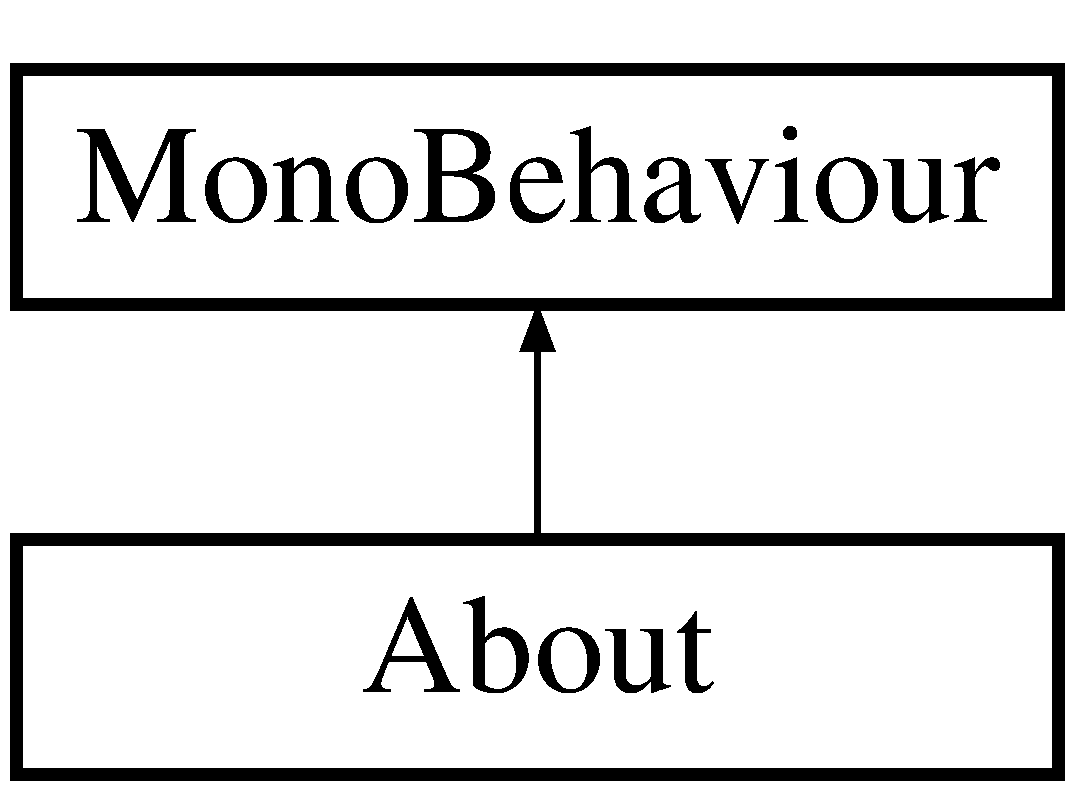
\includegraphics[height=2.000000cm]{class_about}
\end{center}
\end{figure}
\subsection*{Public Member Functions}
\begin{DoxyCompactItemize}
\item 
void \mbox{\hyperlink{class_about_a02d9d9134bd810ba4a3d5e1190be7545}{Load\+Main}} ()
\begin{DoxyCompactList}\small\item\em Load the main menu scene \end{DoxyCompactList}\end{DoxyCompactItemize}


\subsection{Detailed Description}
Class that handles the about scene 



Definition at line 8 of file About.\+cs.



\subsection{Member Function Documentation}
\mbox{\Hypertarget{class_about_a02d9d9134bd810ba4a3d5e1190be7545}\label{class_about_a02d9d9134bd810ba4a3d5e1190be7545}} 
\index{About@{About}!Load\+Main@{Load\+Main}}
\index{Load\+Main@{Load\+Main}!About@{About}}
\subsubsection{\texorpdfstring{Load\+Main()}{LoadMain()}}
{\footnotesize\ttfamily void About.\+Load\+Main (\begin{DoxyParamCaption}{ }\end{DoxyParamCaption})}



Load the main menu scene 



Definition at line 17 of file About.\+cs.



The documentation for this class was generated from the following file\+:\begin{DoxyCompactItemize}
\item 
C\+:/\+Users/louca/\+Documents/\+M\+A\+Dissertation/\+M\+A\+Dissertation/\+M\+A\+Dissertation/\+Assets/\+Classes/\+Scene Specific/About.\+cs\end{DoxyCompactItemize}

\hypertarget{struct_all_overall_player_data}{}\section{All\+Overall\+Player\+Data Struct Reference}
\label{struct_all_overall_player_data}\index{All\+Overall\+Player\+Data@{All\+Overall\+Player\+Data}}


Struct to hold multiple difficulties\textquotesingle{}s overall player data  


\subsection*{Public Attributes}
\begin{DoxyCompactItemize}
\item 
\mbox{\Hypertarget{struct_all_overall_player_data_a8d6556bf610d5f910b198f5593e28c18}\label{struct_all_overall_player_data_a8d6556bf610d5f910b198f5593e28c18}} 
\mbox{\hyperlink{struct_overall_player_data}{Overall\+Player\+Data}} {\bfseries m\+\_\+easy}
\item 
\mbox{\Hypertarget{struct_all_overall_player_data_a6736fb69c263366712bedb10ac16e681}\label{struct_all_overall_player_data_a6736fb69c263366712bedb10ac16e681}} 
\mbox{\hyperlink{struct_overall_player_data}{Overall\+Player\+Data}} {\bfseries m\+\_\+medium}
\item 
\mbox{\Hypertarget{struct_all_overall_player_data_afaf16d31c3a4af551ee3b941e2a3d38e}\label{struct_all_overall_player_data_afaf16d31c3a4af551ee3b941e2a3d38e}} 
\mbox{\hyperlink{struct_overall_player_data}{Overall\+Player\+Data}} {\bfseries m\+\_\+hard}
\end{DoxyCompactItemize}


\subsection{Detailed Description}
Struct to hold multiple difficulties\textquotesingle{}s overall player data 



Definition at line 793 of file Data\+Tracker.\+cs.



The documentation for this struct was generated from the following file\+:\begin{DoxyCompactItemize}
\item 
C\+:/\+Users/louca/\+Documents/\+M\+A\+Dissertation/\+M\+A\+Dissertation/\+M\+A\+Dissertation/\+Assets/\+Classes/\+Database/Data\+Tracker.\+cs\end{DoxyCompactItemize}

\hypertarget{struct_level_generation_1_1_averages}{}\section{Level\+Generation.\+Averages Struct Reference}
\label{struct_level_generation_1_1_averages}\index{Level\+Generation.\+Averages@{Level\+Generation.\+Averages}}


A struct that stores data averages for specific stats  


\subsection*{Public Attributes}
\begin{DoxyCompactItemize}
\item 
\mbox{\Hypertarget{struct_level_generation_1_1_averages_a698be096130b4da9b0f5c16dae691c97}\label{struct_level_generation_1_1_averages_a698be096130b4da9b0f5c16dae691c97}} 
\mbox{\hyperlink{struct_level_generation_1_1_data_averages}{Data\+Averages}} {\bfseries m\+\_\+deaths\+Averages}
\item 
\mbox{\Hypertarget{struct_level_generation_1_1_averages_a733a863af5822b35cd8598f3c05e7bd4}\label{struct_level_generation_1_1_averages_a733a863af5822b35cd8598f3c05e7bd4}} 
\mbox{\hyperlink{struct_level_generation_1_1_data_averages}{Data\+Averages}} {\bfseries m\+\_\+score\+Averages}
\item 
\mbox{\Hypertarget{struct_level_generation_1_1_averages_aa2275a3e93552e7a21c22211a8f0f835}\label{struct_level_generation_1_1_averages_aa2275a3e93552e7a21c22211a8f0f835}} 
\mbox{\hyperlink{struct_level_generation_1_1_data_averages}{Data\+Averages}} {\bfseries m\+\_\+time\+Averages}
\end{DoxyCompactItemize}


\subsection{Detailed Description}
A struct that stores data averages for specific stats 



Definition at line 84 of file Template\+Holder.\+cs.



The documentation for this struct was generated from the following file\+:\begin{DoxyCompactItemize}
\item 
C\+:/\+Users/louca/\+Documents/\+M\+A\+Dissertation/\+M\+A\+Dissertation/\+M\+A\+Dissertation/\+Assets/\+Classes/\+Level Generator/Template\+Holder.\+cs\end{DoxyCompactItemize}

\hypertarget{class_base_averages}{}\section{Base\+Averages Class Reference}
\label{class_base_averages}\index{Base\+Averages@{Base\+Averages}}


A scriptable object that can be used to store the base averages that are used when a new profile is created on the database  


Inheritance diagram for Base\+Averages\+:\begin{figure}[H]
\begin{center}
\leavevmode
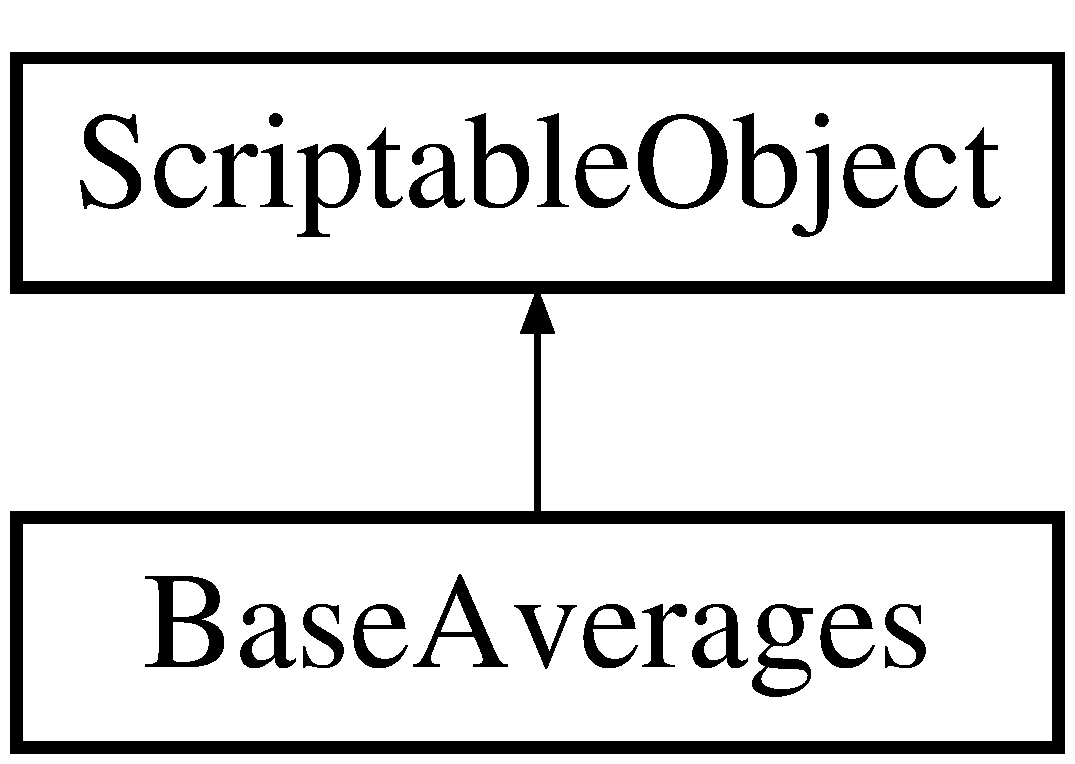
\includegraphics[height=2.000000cm]{class_base_averages}
\end{center}
\end{figure}
\subsection*{Public Member Functions}
\begin{DoxyCompactItemize}
\item 
\mbox{\hyperlink{struct_level_generation_1_1_averages}{Averages}} \mbox{\hyperlink{class_base_averages_af137b781aca1054548d1a04cdb7b2d16}{Get\+Easy\+Averages}} ()
\begin{DoxyCompactList}\small\item\em Get the easy averages \end{DoxyCompactList}\item 
\mbox{\hyperlink{struct_level_generation_1_1_averages}{Averages}} \mbox{\hyperlink{class_base_averages_a1eebd8734dbf18c96295bd93589bcd94}{Get\+Medium\+Averages}} ()
\begin{DoxyCompactList}\small\item\em Get the medium averages \end{DoxyCompactList}\item 
\mbox{\hyperlink{struct_level_generation_1_1_averages}{Averages}} \mbox{\hyperlink{class_base_averages_a5f0bafc5282ea7b0c4842efbe5d077af}{Get\+Hard\+Averages}} ()
\begin{DoxyCompactList}\small\item\em Get the hard averages \end{DoxyCompactList}\end{DoxyCompactItemize}


\subsection{Detailed Description}
A scriptable object that can be used to store the base averages that are used when a new profile is created on the database 



Definition at line 11 of file Base\+Averages.\+cs.



\subsection{Member Function Documentation}
\mbox{\Hypertarget{class_base_averages_af137b781aca1054548d1a04cdb7b2d16}\label{class_base_averages_af137b781aca1054548d1a04cdb7b2d16}} 
\index{Base\+Averages@{Base\+Averages}!Get\+Easy\+Averages@{Get\+Easy\+Averages}}
\index{Get\+Easy\+Averages@{Get\+Easy\+Averages}!Base\+Averages@{Base\+Averages}}
\subsubsection{\texorpdfstring{Get\+Easy\+Averages()}{GetEasyAverages()}}
{\footnotesize\ttfamily \mbox{\hyperlink{struct_level_generation_1_1_averages}{Averages}} Base\+Averages.\+Get\+Easy\+Averages (\begin{DoxyParamCaption}{ }\end{DoxyParamCaption})}



Get the easy averages 

\begin{DoxyReturn}{Returns}
Easy Averages
\end{DoxyReturn}


Definition at line 26 of file Base\+Averages.\+cs.

\mbox{\Hypertarget{class_base_averages_a5f0bafc5282ea7b0c4842efbe5d077af}\label{class_base_averages_a5f0bafc5282ea7b0c4842efbe5d077af}} 
\index{Base\+Averages@{Base\+Averages}!Get\+Hard\+Averages@{Get\+Hard\+Averages}}
\index{Get\+Hard\+Averages@{Get\+Hard\+Averages}!Base\+Averages@{Base\+Averages}}
\subsubsection{\texorpdfstring{Get\+Hard\+Averages()}{GetHardAverages()}}
{\footnotesize\ttfamily \mbox{\hyperlink{struct_level_generation_1_1_averages}{Averages}} Base\+Averages.\+Get\+Hard\+Averages (\begin{DoxyParamCaption}{ }\end{DoxyParamCaption})}



Get the hard averages 

\begin{DoxyReturn}{Returns}
Hard Averages
\end{DoxyReturn}


Definition at line 44 of file Base\+Averages.\+cs.

\mbox{\Hypertarget{class_base_averages_a1eebd8734dbf18c96295bd93589bcd94}\label{class_base_averages_a1eebd8734dbf18c96295bd93589bcd94}} 
\index{Base\+Averages@{Base\+Averages}!Get\+Medium\+Averages@{Get\+Medium\+Averages}}
\index{Get\+Medium\+Averages@{Get\+Medium\+Averages}!Base\+Averages@{Base\+Averages}}
\subsubsection{\texorpdfstring{Get\+Medium\+Averages()}{GetMediumAverages()}}
{\footnotesize\ttfamily \mbox{\hyperlink{struct_level_generation_1_1_averages}{Averages}} Base\+Averages.\+Get\+Medium\+Averages (\begin{DoxyParamCaption}{ }\end{DoxyParamCaption})}



Get the medium averages 

\begin{DoxyReturn}{Returns}
Medium Averages
\end{DoxyReturn}


Definition at line 35 of file Base\+Averages.\+cs.



The documentation for this class was generated from the following file\+:\begin{DoxyCompactItemize}
\item 
C\+:/\+Users/louca/\+Documents/\+M\+A\+Dissertation/\+M\+A\+Dissertation/\+M\+A\+Dissertation/\+Assets/\+Classes/\+Stats/Base\+Averages.\+cs\end{DoxyCompactItemize}

\hypertarget{class_camera_movement}{}\section{Camera\+Movement Class Reference}
\label{class_camera_movement}\index{Camera\+Movement@{Camera\+Movement}}


Moves the camera based on the type of camera needed  


Inheritance diagram for Camera\+Movement\+:\begin{figure}[H]
\begin{center}
\leavevmode
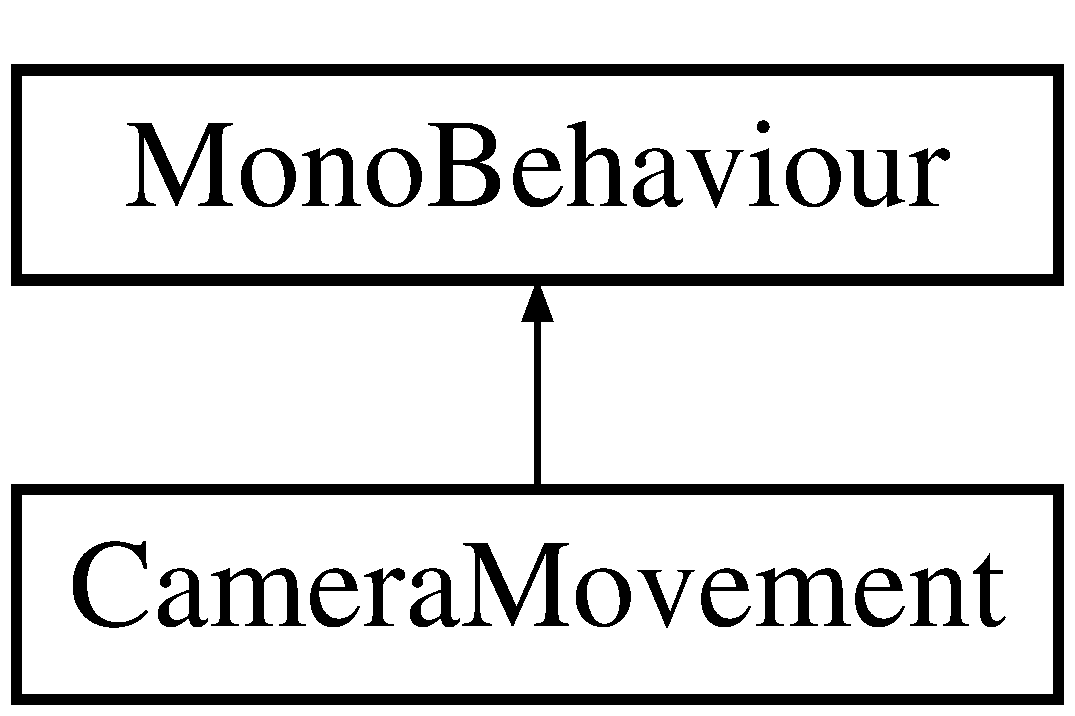
\includegraphics[height=2.000000cm]{class_camera_movement}
\end{center}
\end{figure}
\subsection*{Public Types}
\begin{DoxyCompactItemize}
\item 
enum \mbox{\hyperlink{class_camera_movement_a297cb93f5fc197103c3447dac2340a83}{Camera\+Type}} \{ {\bfseries Room\+To\+Room}
 \}
\begin{DoxyCompactList}\small\item\em Type of camera that will be used \end{DoxyCompactList}\end{DoxyCompactItemize}
\subsection*{Public Member Functions}
\begin{DoxyCompactItemize}
\item 
void \mbox{\hyperlink{class_camera_movement_a9203ee195c435d40bf4fc1de221ed0cd}{Init}} ()
\begin{DoxyCompactList}\small\item\em Handles set up \end{DoxyCompactList}\item 
void \mbox{\hyperlink{class_camera_movement_a198122a1f8e338c1bfe843a0f4f6ce96}{Set\+New\+Room\+Target}} (Transform \+\_\+target\+Transform)
\begin{DoxyCompactList}\small\item\em Set the target room transform \end{DoxyCompactList}\item 
Transform \mbox{\hyperlink{class_camera_movement_a6129de38ce5788f51e7427417bdf7a98}{Has\+Room\+Target}} ()
\begin{DoxyCompactList}\small\item\em Get the target room transform \end{DoxyCompactList}\item 
Transform \mbox{\hyperlink{class_camera_movement_ad707fba6a3e906310efa90dd4285a407}{Current\+Target\+Transform}} ()
\begin{DoxyCompactList}\small\item\em Get the current room trasnform \end{DoxyCompactList}\item 
void \mbox{\hyperlink{class_camera_movement_a22e6e76309d99376ead5b3dffd474938}{Set\+Start\+Room\+Transform}} (Transform \+\_\+start\+Room\+Transform)
\begin{DoxyCompactList}\small\item\em Set the start room transform \end{DoxyCompactList}\item 
void \mbox{\hyperlink{class_camera_movement_a06848ed3326e21d52be8c25ecfe12843}{Reset\+Camera}} ()
\begin{DoxyCompactList}\small\item\em Reset the camera \end{DoxyCompactList}\end{DoxyCompactItemize}


\subsection{Detailed Description}
Moves the camera based on the type of camera needed 



Definition at line 8 of file Camera\+Movement.\+cs.



\subsection{Member Enumeration Documentation}
\mbox{\Hypertarget{class_camera_movement_a297cb93f5fc197103c3447dac2340a83}\label{class_camera_movement_a297cb93f5fc197103c3447dac2340a83}} 
\index{Camera\+Movement@{Camera\+Movement}!Camera\+Type@{Camera\+Type}}
\index{Camera\+Type@{Camera\+Type}!Camera\+Movement@{Camera\+Movement}}
\subsubsection{\texorpdfstring{Camera\+Type}{CameraType}}
{\footnotesize\ttfamily enum \mbox{\hyperlink{class_camera_movement_a297cb93f5fc197103c3447dac2340a83}{Camera\+Movement.\+Camera\+Type}}\hspace{0.3cm}{\ttfamily [strong]}}



Type of camera that will be used 



Definition at line 154 of file Camera\+Movement.\+cs.



\subsection{Member Function Documentation}
\mbox{\Hypertarget{class_camera_movement_ad707fba6a3e906310efa90dd4285a407}\label{class_camera_movement_ad707fba6a3e906310efa90dd4285a407}} 
\index{Camera\+Movement@{Camera\+Movement}!Current\+Target\+Transform@{Current\+Target\+Transform}}
\index{Current\+Target\+Transform@{Current\+Target\+Transform}!Camera\+Movement@{Camera\+Movement}}
\subsubsection{\texorpdfstring{Current\+Target\+Transform()}{CurrentTargetTransform()}}
{\footnotesize\ttfamily Transform Camera\+Movement.\+Current\+Target\+Transform (\begin{DoxyParamCaption}{ }\end{DoxyParamCaption})}



Get the current room trasnform 

\begin{DoxyReturn}{Returns}
Current room transform
\end{DoxyReturn}


Definition at line 125 of file Camera\+Movement.\+cs.

\mbox{\Hypertarget{class_camera_movement_a6129de38ce5788f51e7427417bdf7a98}\label{class_camera_movement_a6129de38ce5788f51e7427417bdf7a98}} 
\index{Camera\+Movement@{Camera\+Movement}!Has\+Room\+Target@{Has\+Room\+Target}}
\index{Has\+Room\+Target@{Has\+Room\+Target}!Camera\+Movement@{Camera\+Movement}}
\subsubsection{\texorpdfstring{Has\+Room\+Target()}{HasRoomTarget()}}
{\footnotesize\ttfamily Transform Camera\+Movement.\+Has\+Room\+Target (\begin{DoxyParamCaption}{ }\end{DoxyParamCaption})}



Get the target room transform 

\begin{DoxyReturn}{Returns}
Target room transform
\end{DoxyReturn}


Definition at line 116 of file Camera\+Movement.\+cs.

\mbox{\Hypertarget{class_camera_movement_a9203ee195c435d40bf4fc1de221ed0cd}\label{class_camera_movement_a9203ee195c435d40bf4fc1de221ed0cd}} 
\index{Camera\+Movement@{Camera\+Movement}!Init@{Init}}
\index{Init@{Init}!Camera\+Movement@{Camera\+Movement}}
\subsubsection{\texorpdfstring{Init()}{Init()}}
{\footnotesize\ttfamily void Camera\+Movement.\+Init (\begin{DoxyParamCaption}{ }\end{DoxyParamCaption})}



Handles set up 



Definition at line 45 of file Camera\+Movement.\+cs.

\mbox{\Hypertarget{class_camera_movement_a06848ed3326e21d52be8c25ecfe12843}\label{class_camera_movement_a06848ed3326e21d52be8c25ecfe12843}} 
\index{Camera\+Movement@{Camera\+Movement}!Reset\+Camera@{Reset\+Camera}}
\index{Reset\+Camera@{Reset\+Camera}!Camera\+Movement@{Camera\+Movement}}
\subsubsection{\texorpdfstring{Reset\+Camera()}{ResetCamera()}}
{\footnotesize\ttfamily void Camera\+Movement.\+Reset\+Camera (\begin{DoxyParamCaption}{ }\end{DoxyParamCaption})}



Reset the camera 



Definition at line 142 of file Camera\+Movement.\+cs.

\mbox{\Hypertarget{class_camera_movement_a198122a1f8e338c1bfe843a0f4f6ce96}\label{class_camera_movement_a198122a1f8e338c1bfe843a0f4f6ce96}} 
\index{Camera\+Movement@{Camera\+Movement}!Set\+New\+Room\+Target@{Set\+New\+Room\+Target}}
\index{Set\+New\+Room\+Target@{Set\+New\+Room\+Target}!Camera\+Movement@{Camera\+Movement}}
\subsubsection{\texorpdfstring{Set\+New\+Room\+Target()}{SetNewRoomTarget()}}
{\footnotesize\ttfamily void Camera\+Movement.\+Set\+New\+Room\+Target (\begin{DoxyParamCaption}\item[{Transform}]{\+\_\+target\+Transform }\end{DoxyParamCaption})}



Set the target room transform 


\begin{DoxyParams}{Parameters}
{\em \+\_\+target\+Transform} & New target transform\\
\hline
\end{DoxyParams}


Definition at line 107 of file Camera\+Movement.\+cs.

\mbox{\Hypertarget{class_camera_movement_a22e6e76309d99376ead5b3dffd474938}\label{class_camera_movement_a22e6e76309d99376ead5b3dffd474938}} 
\index{Camera\+Movement@{Camera\+Movement}!Set\+Start\+Room\+Transform@{Set\+Start\+Room\+Transform}}
\index{Set\+Start\+Room\+Transform@{Set\+Start\+Room\+Transform}!Camera\+Movement@{Camera\+Movement}}
\subsubsection{\texorpdfstring{Set\+Start\+Room\+Transform()}{SetStartRoomTransform()}}
{\footnotesize\ttfamily void Camera\+Movement.\+Set\+Start\+Room\+Transform (\begin{DoxyParamCaption}\item[{Transform}]{\+\_\+start\+Room\+Transform }\end{DoxyParamCaption})}



Set the start room transform 


\begin{DoxyParams}{Parameters}
{\em \+\_\+start\+Room\+Transform} & Start room transform\\
\hline
\end{DoxyParams}


Definition at line 134 of file Camera\+Movement.\+cs.



The documentation for this class was generated from the following file\+:\begin{DoxyCompactItemize}
\item 
C\+:/\+Users/louca/\+Documents/\+M\+A\+Dissertation/\+M\+A\+Dissertation/\+M\+A\+Dissertation/\+Assets/\+Classes/\+Gameplay/Camera\+Movement.\+cs\end{DoxyCompactItemize}

\hypertarget{class_canvas_manager}{}\section{Canvas\+Manager Class Reference}
\label{class_canvas_manager}\index{Canvas\+Manager@{Canvas\+Manager}}


A manager class that allows other classes to access diffent canvases  


Inheritance diagram for Canvas\+Manager\+:\begin{figure}[H]
\begin{center}
\leavevmode
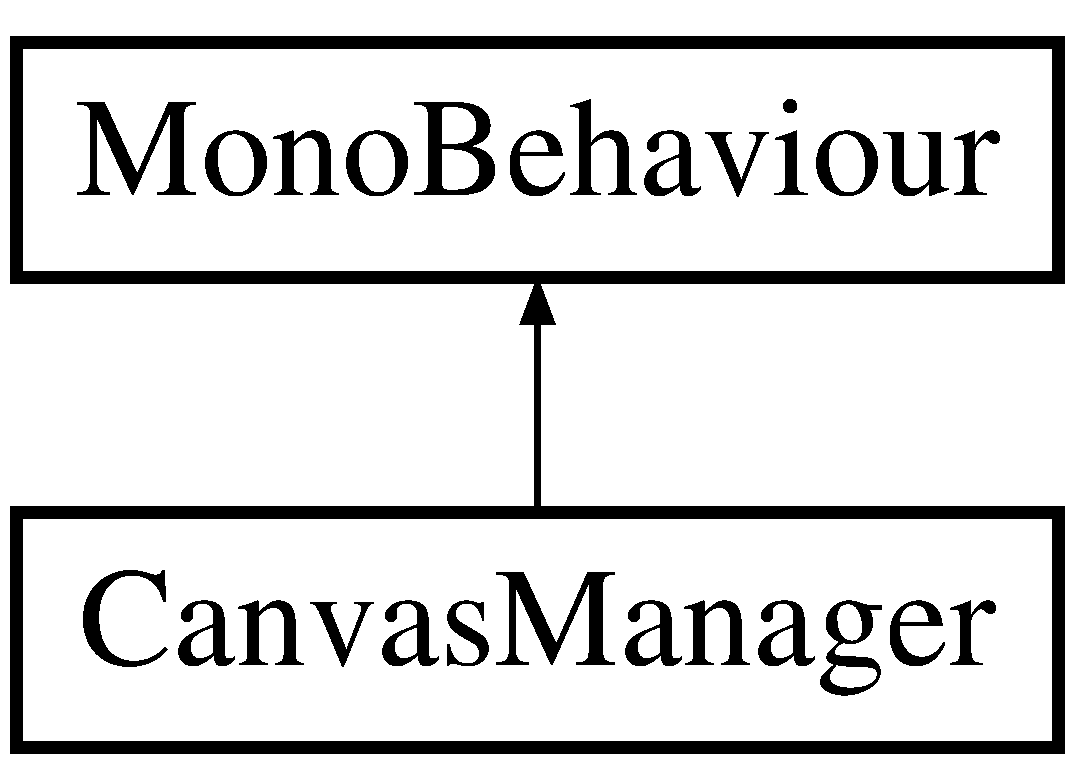
\includegraphics[height=2.000000cm]{class_canvas_manager}
\end{center}
\end{figure}
\subsection*{Public Member Functions}
\begin{DoxyCompactItemize}
\item 
void \mbox{\hyperlink{class_canvas_manager_ae9d3e7181eaefcfe96a7c00772d85f69}{Enable\+Game\+Canvas}} ()
\begin{DoxyCompactList}\small\item\em Enable the game canvas \end{DoxyCompactList}\item 
void \mbox{\hyperlink{class_canvas_manager_a4b45b461a40a6642cbb6ff47b6c13cf5}{Enable\+Pause\+Canvas}} ()
\begin{DoxyCompactList}\small\item\em Enable the pause canvas \end{DoxyCompactList}\item 
void \mbox{\hyperlink{class_canvas_manager_afade6015b931715904f021bc554b65fd}{Exit}} ()
\begin{DoxyCompactList}\small\item\em Exit to the main menu \end{DoxyCompactList}\item 
Game\+Object \mbox{\hyperlink{class_canvas_manager_a029e8183db87b6aa06be208735aff5c6}{Get\+Respawning\+Text}} ()
\begin{DoxyCompactList}\small\item\em Access the respawning text object \end{DoxyCompactList}\item 
\mbox{\hyperlink{class_game_canvas}{Game\+Canvas}} \mbox{\hyperlink{class_canvas_manager_a4ca7162730ba189ec52a772fda4f9a3c}{Get\+Game\+Canvas}} ()
\begin{DoxyCompactList}\small\item\em Access the game canvas \end{DoxyCompactList}\end{DoxyCompactItemize}


\subsection{Detailed Description}
A manager class that allows other classes to access diffent canvases 



Definition at line 9 of file Canvas\+Manager.\+cs.



\subsection{Member Function Documentation}
\mbox{\Hypertarget{class_canvas_manager_ae9d3e7181eaefcfe96a7c00772d85f69}\label{class_canvas_manager_ae9d3e7181eaefcfe96a7c00772d85f69}} 
\index{Canvas\+Manager@{Canvas\+Manager}!Enable\+Game\+Canvas@{Enable\+Game\+Canvas}}
\index{Enable\+Game\+Canvas@{Enable\+Game\+Canvas}!Canvas\+Manager@{Canvas\+Manager}}
\subsubsection{\texorpdfstring{Enable\+Game\+Canvas()}{EnableGameCanvas()}}
{\footnotesize\ttfamily void Canvas\+Manager.\+Enable\+Game\+Canvas (\begin{DoxyParamCaption}{ }\end{DoxyParamCaption})}



Enable the game canvas 



Definition at line 27 of file Canvas\+Manager.\+cs.

\mbox{\Hypertarget{class_canvas_manager_a4b45b461a40a6642cbb6ff47b6c13cf5}\label{class_canvas_manager_a4b45b461a40a6642cbb6ff47b6c13cf5}} 
\index{Canvas\+Manager@{Canvas\+Manager}!Enable\+Pause\+Canvas@{Enable\+Pause\+Canvas}}
\index{Enable\+Pause\+Canvas@{Enable\+Pause\+Canvas}!Canvas\+Manager@{Canvas\+Manager}}
\subsubsection{\texorpdfstring{Enable\+Pause\+Canvas()}{EnablePauseCanvas()}}
{\footnotesize\ttfamily void Canvas\+Manager.\+Enable\+Pause\+Canvas (\begin{DoxyParamCaption}{ }\end{DoxyParamCaption})}



Enable the pause canvas 



Definition at line 36 of file Canvas\+Manager.\+cs.

\mbox{\Hypertarget{class_canvas_manager_afade6015b931715904f021bc554b65fd}\label{class_canvas_manager_afade6015b931715904f021bc554b65fd}} 
\index{Canvas\+Manager@{Canvas\+Manager}!Exit@{Exit}}
\index{Exit@{Exit}!Canvas\+Manager@{Canvas\+Manager}}
\subsubsection{\texorpdfstring{Exit()}{Exit()}}
{\footnotesize\ttfamily void Canvas\+Manager.\+Exit (\begin{DoxyParamCaption}{ }\end{DoxyParamCaption})}



Exit to the main menu 



Definition at line 45 of file Canvas\+Manager.\+cs.

\mbox{\Hypertarget{class_canvas_manager_a4ca7162730ba189ec52a772fda4f9a3c}\label{class_canvas_manager_a4ca7162730ba189ec52a772fda4f9a3c}} 
\index{Canvas\+Manager@{Canvas\+Manager}!Get\+Game\+Canvas@{Get\+Game\+Canvas}}
\index{Get\+Game\+Canvas@{Get\+Game\+Canvas}!Canvas\+Manager@{Canvas\+Manager}}
\subsubsection{\texorpdfstring{Get\+Game\+Canvas()}{GetGameCanvas()}}
{\footnotesize\ttfamily \mbox{\hyperlink{class_game_canvas}{Game\+Canvas}} Canvas\+Manager.\+Get\+Game\+Canvas (\begin{DoxyParamCaption}{ }\end{DoxyParamCaption})}



Access the game canvas 

\begin{DoxyReturn}{Returns}
Game Canvas object
\end{DoxyReturn}


Definition at line 63 of file Canvas\+Manager.\+cs.

\mbox{\Hypertarget{class_canvas_manager_a029e8183db87b6aa06be208735aff5c6}\label{class_canvas_manager_a029e8183db87b6aa06be208735aff5c6}} 
\index{Canvas\+Manager@{Canvas\+Manager}!Get\+Respawning\+Text@{Get\+Respawning\+Text}}
\index{Get\+Respawning\+Text@{Get\+Respawning\+Text}!Canvas\+Manager@{Canvas\+Manager}}
\subsubsection{\texorpdfstring{Get\+Respawning\+Text()}{GetRespawningText()}}
{\footnotesize\ttfamily Game\+Object Canvas\+Manager.\+Get\+Respawning\+Text (\begin{DoxyParamCaption}{ }\end{DoxyParamCaption})}



Access the respawning text object 

\begin{DoxyReturn}{Returns}
Respawning text object
\end{DoxyReturn}


Definition at line 54 of file Canvas\+Manager.\+cs.



The documentation for this class was generated from the following file\+:\begin{DoxyCompactItemize}
\item 
C\+:/\+Users/louca/\+Documents/\+M\+A\+Dissertation/\+M\+A\+Dissertation/\+M\+A\+Dissertation/\+Assets/\+Classes/\+U\+I/Canvas\+Manager.\+cs\end{DoxyCompactItemize}

\hypertarget{class_character}{}\section{Character Class Reference}
\label{class_character}\index{Character@{Character}}


Base class for player and enemies  


Inheritance diagram for Character\+:\begin{figure}[H]
\begin{center}
\leavevmode
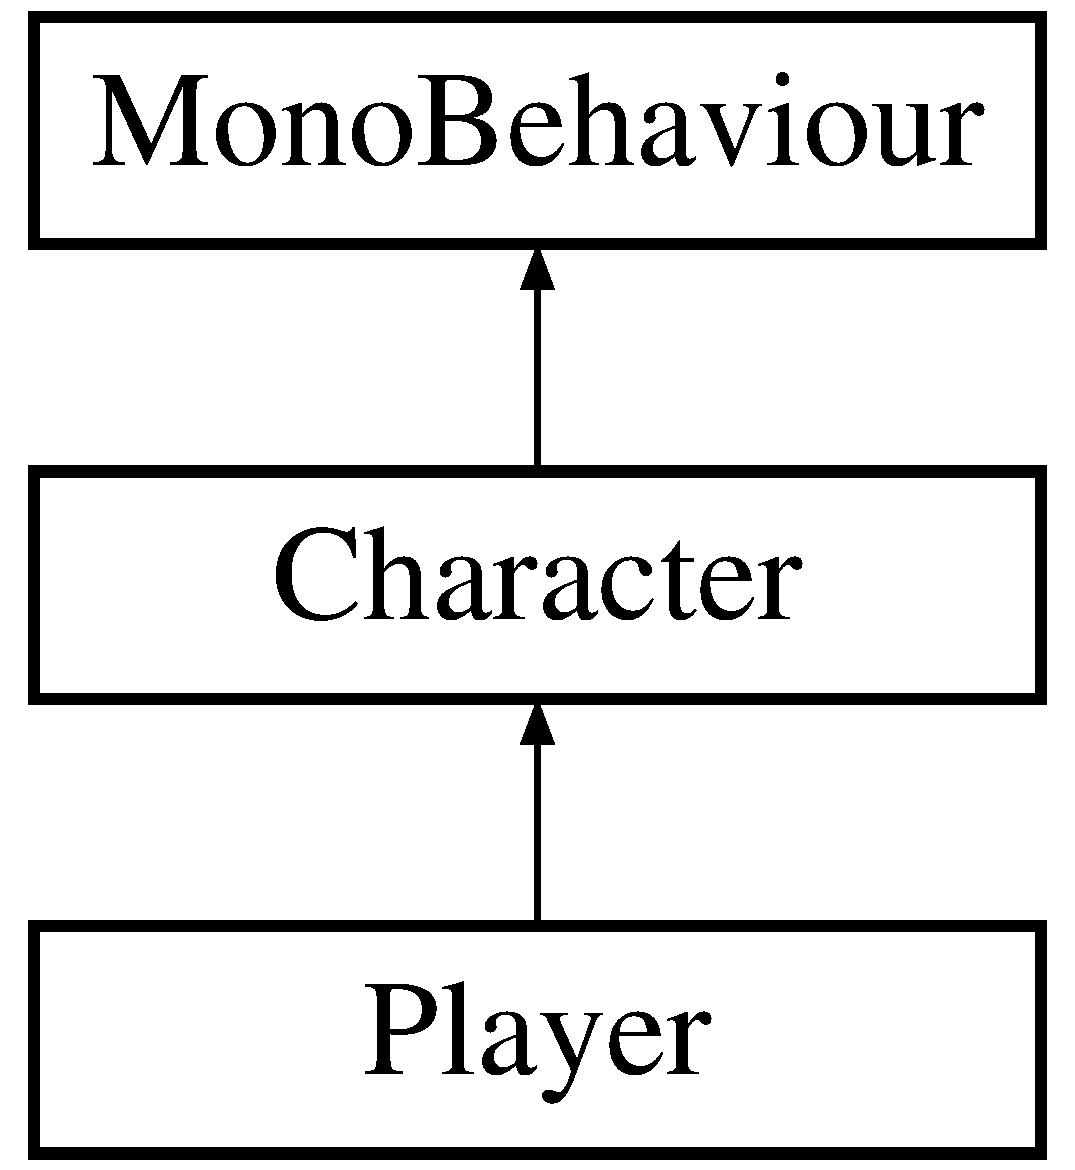
\includegraphics[height=3.000000cm]{class_character}
\end{center}
\end{figure}
\subsection*{Protected Member Functions}
\begin{DoxyCompactItemize}
\item 
virtual void \mbox{\hyperlink{class_character_a7cca5d1f141f2f46a1d087fd3e28a953}{Awake}} ()
\begin{DoxyCompactList}\small\item\em Handles inital set up \end{DoxyCompactList}\item 
\mbox{\Hypertarget{class_character_a98bebdb5d37a51749749f0684f14a6ca}\label{class_character_a98bebdb5d37a51749749f0684f14a6ca}} 
virtual void {\bfseries Start} ()
\item 
\mbox{\Hypertarget{class_character_aeabbd75a8c44cc4542112852ca735f2d}\label{class_character_aeabbd75a8c44cc4542112852ca735f2d}} 
virtual void {\bfseries Update} ()
\item 
virtual void \mbox{\hyperlink{class_character_ad90105ab5e234884e5bca7ce5bd2c50e}{Fixed\+Update}} ()
\begin{DoxyCompactList}\small\item\em Fixed update is called once per fixed frame \end{DoxyCompactList}\end{DoxyCompactItemize}
\subsection*{Protected Attributes}
\begin{DoxyCompactItemize}
\item 
\mbox{\Hypertarget{class_character_ae6f38ea3ad77f6aeba55631d8a47f089}\label{class_character_ae6f38ea3ad77f6aeba55631d8a47f089}} 
\mbox{\hyperlink{struct_character_start_data}{Character\+Start\+Data}} {\bfseries m\+\_\+character\+Data}
\item 
\mbox{\Hypertarget{class_character_a0049d5b1f387150dbe1086086fcaea4c}\label{class_character_a0049d5b1f387150dbe1086086fcaea4c}} 
float {\bfseries m\+\_\+gravity}
\item 
\mbox{\Hypertarget{class_character_a694ba48446eed2ff9ce2354f83f2072c}\label{class_character_a694ba48446eed2ff9ce2354f83f2072c}} 
int {\bfseries m\+\_\+current\+Health}
\item 
\mbox{\Hypertarget{class_character_a98899aa78f445adc994fb39a50f37fc4}\label{class_character_a98899aa78f445adc994fb39a50f37fc4}} 
Rigidbody2D {\bfseries m\+\_\+rigid\+Body}
\item 
\mbox{\Hypertarget{class_character_a3522770974fe60235263b7050b30e1c8}\label{class_character_a3522770974fe60235263b7050b30e1c8}} 
Sprite\+Renderer {\bfseries m\+\_\+renderer}
\end{DoxyCompactItemize}


\subsection{Detailed Description}
Base class for player and enemies 



Definition at line 8 of file Character.\+cs.



\subsection{Member Function Documentation}
\mbox{\Hypertarget{class_character_a7cca5d1f141f2f46a1d087fd3e28a953}\label{class_character_a7cca5d1f141f2f46a1d087fd3e28a953}} 
\index{Character@{Character}!Awake@{Awake}}
\index{Awake@{Awake}!Character@{Character}}
\subsubsection{\texorpdfstring{Awake()}{Awake()}}
{\footnotesize\ttfamily virtual void Character.\+Awake (\begin{DoxyParamCaption}{ }\end{DoxyParamCaption})\hspace{0.3cm}{\ttfamily [protected]}, {\ttfamily [virtual]}}



Handles inital set up 



Reimplemented in \mbox{\hyperlink{class_player_a21d9f4bbd86a4a1aaa8844917270aefb}{Player}}.



Definition at line 25 of file Character.\+cs.

\mbox{\Hypertarget{class_character_ad90105ab5e234884e5bca7ce5bd2c50e}\label{class_character_ad90105ab5e234884e5bca7ce5bd2c50e}} 
\index{Character@{Character}!Fixed\+Update@{Fixed\+Update}}
\index{Fixed\+Update@{Fixed\+Update}!Character@{Character}}
\subsubsection{\texorpdfstring{Fixed\+Update()}{FixedUpdate()}}
{\footnotesize\ttfamily virtual void Character.\+Fixed\+Update (\begin{DoxyParamCaption}{ }\end{DoxyParamCaption})\hspace{0.3cm}{\ttfamily [protected]}, {\ttfamily [virtual]}}



Fixed update is called once per fixed frame 



Reimplemented in \mbox{\hyperlink{class_player_a9f719f4557355ff498cc7ff6d3723a84}{Player}}.



Definition at line 46 of file Character.\+cs.



The documentation for this class was generated from the following file\+:\begin{DoxyCompactItemize}
\item 
C\+:/\+Users/louca/\+Documents/\+M\+A\+Dissertation/\+M\+A\+Dissertation/\+M\+A\+Dissertation/\+Assets/\+Classes/\+Gameplay/Character.\+cs\end{DoxyCompactItemize}

\hypertarget{struct_character_start_data}{}\section{Character\+Start\+Data Struct Reference}
\label{struct_character_start_data}\index{Character\+Start\+Data@{Character\+Start\+Data}}


Data to initialise the character with  


\subsection*{Public Attributes}
\begin{DoxyCompactItemize}
\item 
\mbox{\Hypertarget{struct_character_start_data_a97d16f5fe4a9be0e6a010ad0fde5ac86}\label{struct_character_start_data_a97d16f5fe4a9be0e6a010ad0fde5ac86}} 
int {\bfseries m\+\_\+health}
\item 
\mbox{\Hypertarget{struct_character_start_data_ae14b830ff22f4ac423ac786508e3575f}\label{struct_character_start_data_ae14b830ff22f4ac423ac786508e3575f}} 
float {\bfseries m\+\_\+move\+Speed}
\item 
\mbox{\Hypertarget{struct_character_start_data_a708b3c236235a419bb60048ea399845a}\label{struct_character_start_data_a708b3c236235a419bb60048ea399845a}} 
float {\bfseries m\+\_\+jump\+Speed}
\item 
\mbox{\Hypertarget{struct_character_start_data_ae6795c9f129c702fddddaa554532d50e}\label{struct_character_start_data_ae6795c9f129c702fddddaa554532d50e}} 
Sprite {\bfseries m\+\_\+idle\+Sprite}
\item 
\mbox{\Hypertarget{struct_character_start_data_a3c7987adaffb5bebbd3142fbe3f9694f}\label{struct_character_start_data_a3c7987adaffb5bebbd3142fbe3f9694f}} 
Sprite {\bfseries m\+\_\+right\+Sprite}
\item 
\mbox{\Hypertarget{struct_character_start_data_ac97181cdb1db77dcfda4c944bd122ed4}\label{struct_character_start_data_ac97181cdb1db77dcfda4c944bd122ed4}} 
Sprite {\bfseries m\+\_\+left\+Sprite}
\end{DoxyCompactItemize}


\subsection{Detailed Description}
Data to initialise the character with 



Definition at line 79 of file Character.\+cs.



The documentation for this struct was generated from the following file\+:\begin{DoxyCompactItemize}
\item 
C\+:/\+Users/louca/\+Documents/\+M\+A\+Dissertation/\+M\+A\+Dissertation/\+M\+A\+Dissertation/\+Assets/\+Classes/\+Gameplay/Character.\+cs\end{DoxyCompactItemize}

\hypertarget{class_collectable}{}\section{Collectable Class Reference}
\label{class_collectable}\index{Collectable@{Collectable}}


An object that a player can pick up to get a higher score  


Inheritance diagram for Collectable\+:\begin{figure}[H]
\begin{center}
\leavevmode
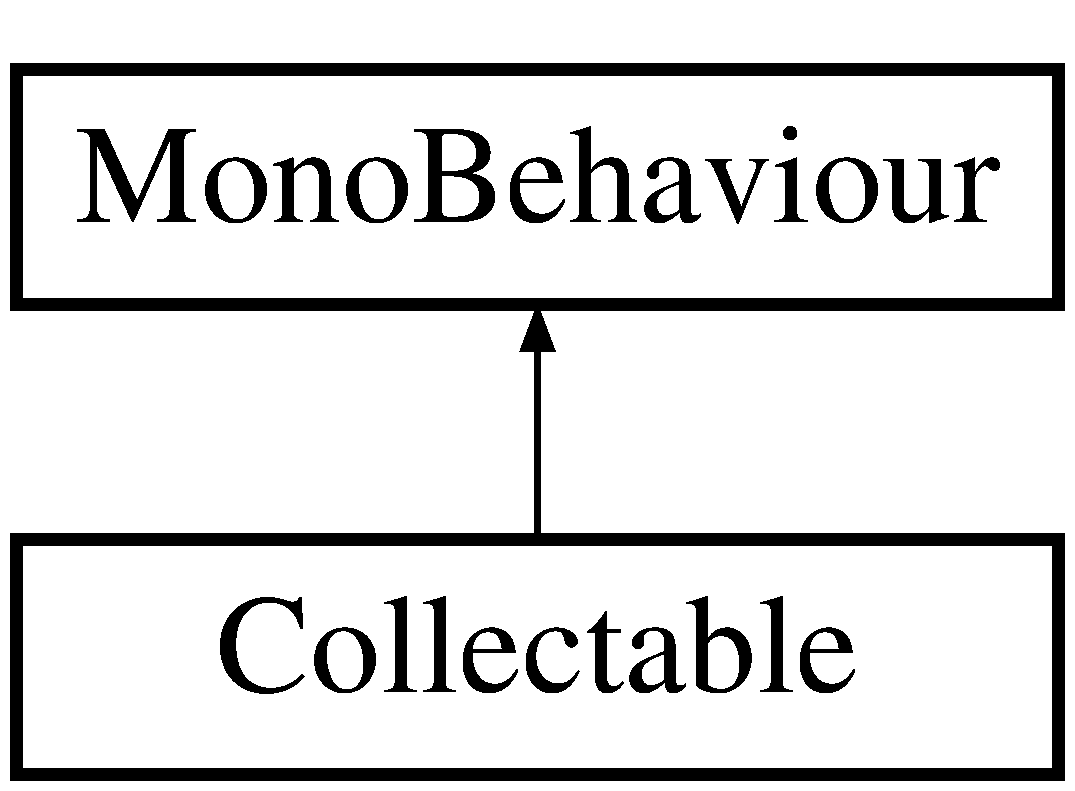
\includegraphics[height=2.000000cm]{class_collectable}
\end{center}
\end{figure}
\subsection*{Public Member Functions}
\begin{DoxyCompactItemize}
\item 
int \mbox{\hyperlink{class_collectable_a6ee23f6709322822b8334c014537e555}{Collect}} ()
\begin{DoxyCompactList}\small\item\em Returns a score value to be added to the overall score \end{DoxyCompactList}\item 
int \mbox{\hyperlink{class_collectable_a11287fc9a8dda57c70095d56f53aa329}{Get\+Spawn\+Rate}} ()
\begin{DoxyCompactList}\small\item\em Returns the spawn rate for the specific collectable \end{DoxyCompactList}\end{DoxyCompactItemize}


\subsection{Detailed Description}
An object that a player can pick up to get a higher score 



Definition at line 8 of file Collectable.\+cs.



\subsection{Member Function Documentation}
\mbox{\Hypertarget{class_collectable_a6ee23f6709322822b8334c014537e555}\label{class_collectable_a6ee23f6709322822b8334c014537e555}} 
\index{Collectable@{Collectable}!Collect@{Collect}}
\index{Collect@{Collect}!Collectable@{Collectable}}
\subsubsection{\texorpdfstring{Collect()}{Collect()}}
{\footnotesize\ttfamily int Collectable.\+Collect (\begin{DoxyParamCaption}{ }\end{DoxyParamCaption})}



Returns a score value to be added to the overall score 

\begin{DoxyReturn}{Returns}
The amount of points given when picking up this object
\end{DoxyReturn}


Definition at line 21 of file Collectable.\+cs.

\mbox{\Hypertarget{class_collectable_a11287fc9a8dda57c70095d56f53aa329}\label{class_collectable_a11287fc9a8dda57c70095d56f53aa329}} 
\index{Collectable@{Collectable}!Get\+Spawn\+Rate@{Get\+Spawn\+Rate}}
\index{Get\+Spawn\+Rate@{Get\+Spawn\+Rate}!Collectable@{Collectable}}
\subsubsection{\texorpdfstring{Get\+Spawn\+Rate()}{GetSpawnRate()}}
{\footnotesize\ttfamily int Collectable.\+Get\+Spawn\+Rate (\begin{DoxyParamCaption}{ }\end{DoxyParamCaption})}



Returns the spawn rate for the specific collectable 

\begin{DoxyReturn}{Returns}
Spawn Rate
\end{DoxyReturn}


Definition at line 30 of file Collectable.\+cs.



The documentation for this class was generated from the following file\+:\begin{DoxyCompactItemize}
\item 
C\+:/\+Users/louca/\+Documents/\+M\+A\+Dissertation/\+M\+A\+Dissertation/\+M\+A\+Dissertation/\+Assets/\+Classes/\+Gameplay/Collectable.\+cs\end{DoxyCompactItemize}

\hypertarget{class_control_scheme}{}\section{Control\+Scheme Class Reference}
\label{class_control_scheme}\index{Control\+Scheme@{Control\+Scheme}}


A class that controls the control scheme scene  


Inheritance diagram for Control\+Scheme\+:\begin{figure}[H]
\begin{center}
\leavevmode
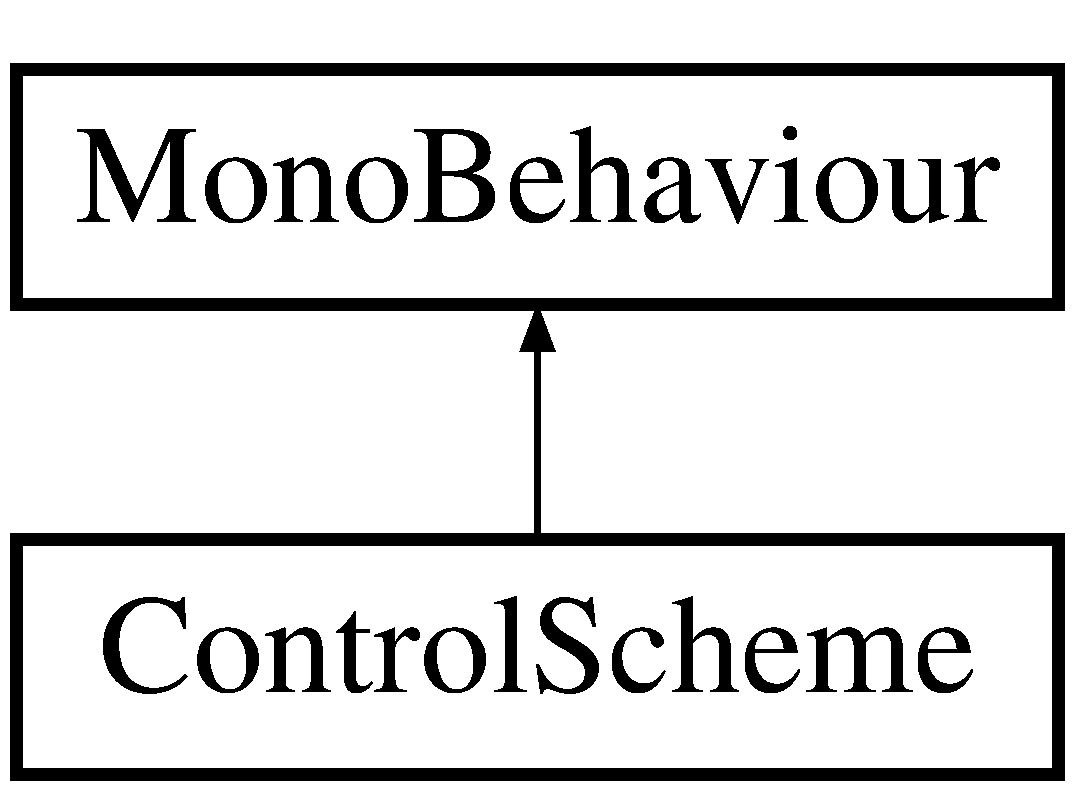
\includegraphics[height=2.000000cm]{class_control_scheme}
\end{center}
\end{figure}
\subsection*{Public Member Functions}
\begin{DoxyCompactItemize}
\item 
void \mbox{\hyperlink{class_control_scheme_addb29fabf571ce6558a7a09b58ab7b3f}{Load\+Game}} ()
\begin{DoxyCompactList}\small\item\em Load the game scene \end{DoxyCompactList}\end{DoxyCompactItemize}


\subsection{Detailed Description}
A class that controls the control scheme scene 



Definition at line 11 of file Control\+Scheme.\+cs.



\subsection{Member Function Documentation}
\mbox{\Hypertarget{class_control_scheme_addb29fabf571ce6558a7a09b58ab7b3f}\label{class_control_scheme_addb29fabf571ce6558a7a09b58ab7b3f}} 
\index{Control\+Scheme@{Control\+Scheme}!Load\+Game@{Load\+Game}}
\index{Load\+Game@{Load\+Game}!Control\+Scheme@{Control\+Scheme}}
\subsubsection{\texorpdfstring{Load\+Game()}{LoadGame()}}
{\footnotesize\ttfamily void Control\+Scheme.\+Load\+Game (\begin{DoxyParamCaption}{ }\end{DoxyParamCaption})}



Load the game scene 



Definition at line 75 of file Control\+Scheme.\+cs.



The documentation for this class was generated from the following file\+:\begin{DoxyCompactItemize}
\item 
C\+:/\+Users/louca/\+Documents/\+M\+A\+Dissertation/\+M\+A\+Dissertation/\+M\+A\+Dissertation/\+Assets/\+Classes/\+Scene Specific/Control\+Scheme.\+cs\end{DoxyCompactItemize}

\hypertarget{struct_level_generation_1_1_data_averages}{}\section{Level\+Generation.\+Data\+Averages Struct Reference}
\label{struct_level_generation_1_1_data_averages}\index{Level\+Generation.\+Data\+Averages@{Level\+Generation.\+Data\+Averages}}


A struct that stores an average and standard deviation value  


\subsection*{Public Attributes}
\begin{DoxyCompactItemize}
\item 
\mbox{\Hypertarget{struct_level_generation_1_1_data_averages_a937d380bef416a107dc8d00da75206b0}\label{struct_level_generation_1_1_data_averages_a937d380bef416a107dc8d00da75206b0}} 
float {\bfseries m\+\_\+average}
\item 
\mbox{\Hypertarget{struct_level_generation_1_1_data_averages_a51766c79c560982148bac560a2ae789d}\label{struct_level_generation_1_1_data_averages_a51766c79c560982148bac560a2ae789d}} 
float {\bfseries m\+\_\+standard\+Deviation}
\end{DoxyCompactItemize}


\subsection{Detailed Description}
A struct that stores an average and standard deviation value 



Definition at line 74 of file Template\+Holder.\+cs.



The documentation for this struct was generated from the following file\+:\begin{DoxyCompactItemize}
\item 
C\+:/\+Users/louca/\+Documents/\+M\+A\+Dissertation/\+M\+A\+Dissertation/\+M\+A\+Dissertation/\+Assets/\+Classes/\+Level Generator/Template\+Holder.\+cs\end{DoxyCompactItemize}

\hypertarget{class_database_manager}{}\section{Database\+Manager Class Reference}
\label{class_database_manager}\index{Database\+Manager@{Database\+Manager}}


Singleton class to handle the linking between the game and the firebase database  


Inheritance diagram for Database\+Manager\+:\begin{figure}[H]
\begin{center}
\leavevmode
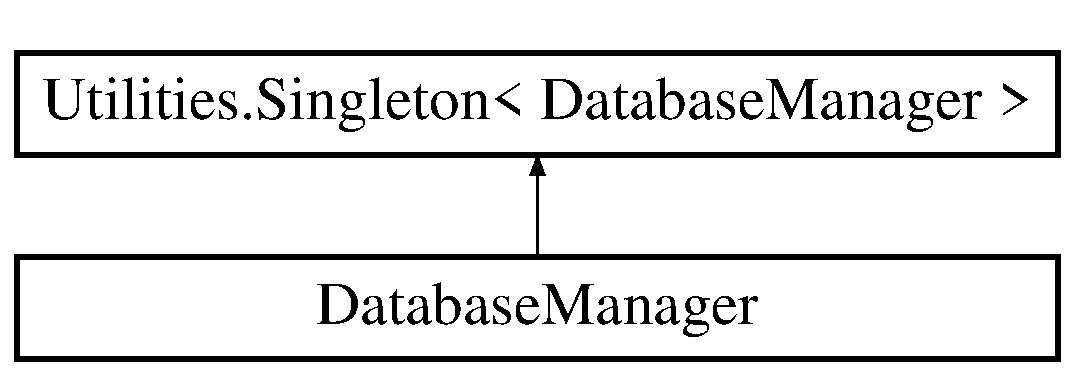
\includegraphics[height=2.000000cm]{class_database_manager}
\end{center}
\end{figure}
\subsection*{Public Member Functions}
\begin{DoxyCompactItemize}
\item 
Database\+Reference \mbox{\hyperlink{class_database_manager_a14c609571c0d42f0735da6e8c8ff92c0}{Get\+Database\+Reference}} ()
\begin{DoxyCompactList}\small\item\em Allow other classes to access the database reference \end{DoxyCompactList}\item 
bool \mbox{\hyperlink{class_database_manager_ad0baa3bf8e05288ba738646770672b34}{Is\+Database\+Ready}} ()
\begin{DoxyCompactList}\small\item\em Allows other classes to check if the database is ready \end{DoxyCompactList}\item 
int \mbox{\hyperlink{class_database_manager_a4c6fcf71634e8465870bb7468da305e4}{Get\+Playthrough\+Id}} ()
\begin{DoxyCompactList}\small\item\em Allows other classes to access the playthrough id \end{DoxyCompactList}\item 
void \mbox{\hyperlink{class_database_manager_a8215a2e17e479aa9c2f76bdf1a18a018}{Increase\+Playthrough\+Id}} ()
\begin{DoxyCompactList}\small\item\em Increases the playthrough count \end{DoxyCompactList}\item 
\mbox{\hyperlink{struct_level_generation_1_1_averages}{Averages}} \mbox{\hyperlink{class_database_manager_a8b767bfbaf23f5ebc65fb3616db8932b}{Access\+Init\+Easy\+Averages}} ()
\begin{DoxyCompactList}\small\item\em Access the easy averages \end{DoxyCompactList}\item 
\mbox{\hyperlink{struct_level_generation_1_1_averages}{Averages}} \mbox{\hyperlink{class_database_manager_a7e11fd2b33cec339e52eb3df7b595da1}{Access\+Init\+Medium\+Averages}} ()
\begin{DoxyCompactList}\small\item\em Access the medium averages \end{DoxyCompactList}\item 
\mbox{\hyperlink{struct_level_generation_1_1_averages}{Averages}} \mbox{\hyperlink{class_database_manager_a61d0614a2d858005a6c3abac1283c8f2}{Access\+Init\+Hard\+Averages}} ()
\begin{DoxyCompactList}\small\item\em Access the hard averages \end{DoxyCompactList}\item 
string \mbox{\hyperlink{class_database_manager_a3ecc1e7d30ba7c71922588dd7a03c8cb}{Access\+Group\+Name}} ()
\begin{DoxyCompactList}\small\item\em Access the group ID \end{DoxyCompactList}\item 
string \mbox{\hyperlink{class_database_manager_a78fbe5d16d91f8a9da73c348518af5fb}{Access\+Unique\+Id}} ()
\begin{DoxyCompactList}\small\item\em Access the unique device ID \end{DoxyCompactList}\item 
string \mbox{\hyperlink{class_database_manager_a59fd27d4114804a39d197da3b95fa2de}{Access\+Id}} ()
\begin{DoxyCompactList}\small\item\em Access the player ID \end{DoxyCompactList}\end{DoxyCompactItemize}
\subsection*{Protected Member Functions}
\begin{DoxyCompactItemize}
\item 
override void \mbox{\hyperlink{class_database_manager_ab6b2a5348b157b217b1ee38a468a3167}{Awake}} ()
\begin{DoxyCompactList}\small\item\em Database initialisation and singleton set up \end{DoxyCompactList}\end{DoxyCompactItemize}
\subsection*{Additional Inherited Members}


\subsection{Detailed Description}
Singleton class to handle the linking between the game and the firebase database 



Definition at line 13 of file Database\+Manager.\+cs.



\subsection{Member Function Documentation}
\mbox{\Hypertarget{class_database_manager_a3ecc1e7d30ba7c71922588dd7a03c8cb}\label{class_database_manager_a3ecc1e7d30ba7c71922588dd7a03c8cb}} 
\index{Database\+Manager@{Database\+Manager}!Access\+Group\+Name@{Access\+Group\+Name}}
\index{Access\+Group\+Name@{Access\+Group\+Name}!Database\+Manager@{Database\+Manager}}
\subsubsection{\texorpdfstring{Access\+Group\+Name()}{AccessGroupName()}}
{\footnotesize\ttfamily string Database\+Manager.\+Access\+Group\+Name (\begin{DoxyParamCaption}{ }\end{DoxyParamCaption})}



Access the group ID 

\begin{DoxyReturn}{Returns}
Group ID
\end{DoxyReturn}


Definition at line 339 of file Database\+Manager.\+cs.

\mbox{\Hypertarget{class_database_manager_a59fd27d4114804a39d197da3b95fa2de}\label{class_database_manager_a59fd27d4114804a39d197da3b95fa2de}} 
\index{Database\+Manager@{Database\+Manager}!Access\+Id@{Access\+Id}}
\index{Access\+Id@{Access\+Id}!Database\+Manager@{Database\+Manager}}
\subsubsection{\texorpdfstring{Access\+Id()}{AccessId()}}
{\footnotesize\ttfamily string Database\+Manager.\+Access\+Id (\begin{DoxyParamCaption}{ }\end{DoxyParamCaption})}



Access the player ID 

\begin{DoxyReturn}{Returns}
Returns the group ID or the unique ID
\end{DoxyReturn}


Definition at line 357 of file Database\+Manager.\+cs.

\mbox{\Hypertarget{class_database_manager_a8b767bfbaf23f5ebc65fb3616db8932b}\label{class_database_manager_a8b767bfbaf23f5ebc65fb3616db8932b}} 
\index{Database\+Manager@{Database\+Manager}!Access\+Init\+Easy\+Averages@{Access\+Init\+Easy\+Averages}}
\index{Access\+Init\+Easy\+Averages@{Access\+Init\+Easy\+Averages}!Database\+Manager@{Database\+Manager}}
\subsubsection{\texorpdfstring{Access\+Init\+Easy\+Averages()}{AccessInitEasyAverages()}}
{\footnotesize\ttfamily \mbox{\hyperlink{struct_level_generation_1_1_averages}{Averages}} Database\+Manager.\+Access\+Init\+Easy\+Averages (\begin{DoxyParamCaption}{ }\end{DoxyParamCaption})}



Access the easy averages 

\begin{DoxyReturn}{Returns}
Easy averages
\end{DoxyReturn}


Definition at line 312 of file Database\+Manager.\+cs.

\mbox{\Hypertarget{class_database_manager_a61d0614a2d858005a6c3abac1283c8f2}\label{class_database_manager_a61d0614a2d858005a6c3abac1283c8f2}} 
\index{Database\+Manager@{Database\+Manager}!Access\+Init\+Hard\+Averages@{Access\+Init\+Hard\+Averages}}
\index{Access\+Init\+Hard\+Averages@{Access\+Init\+Hard\+Averages}!Database\+Manager@{Database\+Manager}}
\subsubsection{\texorpdfstring{Access\+Init\+Hard\+Averages()}{AccessInitHardAverages()}}
{\footnotesize\ttfamily \mbox{\hyperlink{struct_level_generation_1_1_averages}{Averages}} Database\+Manager.\+Access\+Init\+Hard\+Averages (\begin{DoxyParamCaption}{ }\end{DoxyParamCaption})}



Access the hard averages 

\begin{DoxyReturn}{Returns}
Hard averages
\end{DoxyReturn}


Definition at line 330 of file Database\+Manager.\+cs.

\mbox{\Hypertarget{class_database_manager_a7e11fd2b33cec339e52eb3df7b595da1}\label{class_database_manager_a7e11fd2b33cec339e52eb3df7b595da1}} 
\index{Database\+Manager@{Database\+Manager}!Access\+Init\+Medium\+Averages@{Access\+Init\+Medium\+Averages}}
\index{Access\+Init\+Medium\+Averages@{Access\+Init\+Medium\+Averages}!Database\+Manager@{Database\+Manager}}
\subsubsection{\texorpdfstring{Access\+Init\+Medium\+Averages()}{AccessInitMediumAverages()}}
{\footnotesize\ttfamily \mbox{\hyperlink{struct_level_generation_1_1_averages}{Averages}} Database\+Manager.\+Access\+Init\+Medium\+Averages (\begin{DoxyParamCaption}{ }\end{DoxyParamCaption})}



Access the medium averages 

\begin{DoxyReturn}{Returns}
Medium averages
\end{DoxyReturn}


Definition at line 321 of file Database\+Manager.\+cs.

\mbox{\Hypertarget{class_database_manager_a78fbe5d16d91f8a9da73c348518af5fb}\label{class_database_manager_a78fbe5d16d91f8a9da73c348518af5fb}} 
\index{Database\+Manager@{Database\+Manager}!Access\+Unique\+Id@{Access\+Unique\+Id}}
\index{Access\+Unique\+Id@{Access\+Unique\+Id}!Database\+Manager@{Database\+Manager}}
\subsubsection{\texorpdfstring{Access\+Unique\+Id()}{AccessUniqueId()}}
{\footnotesize\ttfamily string Database\+Manager.\+Access\+Unique\+Id (\begin{DoxyParamCaption}{ }\end{DoxyParamCaption})}



Access the unique device ID 

\begin{DoxyReturn}{Returns}
Unique device ID
\end{DoxyReturn}


Definition at line 348 of file Database\+Manager.\+cs.

\mbox{\Hypertarget{class_database_manager_ab6b2a5348b157b217b1ee38a468a3167}\label{class_database_manager_ab6b2a5348b157b217b1ee38a468a3167}} 
\index{Database\+Manager@{Database\+Manager}!Awake@{Awake}}
\index{Awake@{Awake}!Database\+Manager@{Database\+Manager}}
\subsubsection{\texorpdfstring{Awake()}{Awake()}}
{\footnotesize\ttfamily override void Database\+Manager.\+Awake (\begin{DoxyParamCaption}{ }\end{DoxyParamCaption})\hspace{0.3cm}{\ttfamily [protected]}, {\ttfamily [virtual]}}



Database initialisation and singleton set up 



Reimplemented from \mbox{\hyperlink{class_utilities_1_1_singleton_a634b915d7ac492899512de602d59e650}{Utilities.\+Singleton$<$ Database\+Manager $>$}}.



Definition at line 37 of file Database\+Manager.\+cs.

\mbox{\Hypertarget{class_database_manager_a14c609571c0d42f0735da6e8c8ff92c0}\label{class_database_manager_a14c609571c0d42f0735da6e8c8ff92c0}} 
\index{Database\+Manager@{Database\+Manager}!Get\+Database\+Reference@{Get\+Database\+Reference}}
\index{Get\+Database\+Reference@{Get\+Database\+Reference}!Database\+Manager@{Database\+Manager}}
\subsubsection{\texorpdfstring{Get\+Database\+Reference()}{GetDatabaseReference()}}
{\footnotesize\ttfamily Database\+Reference Database\+Manager.\+Get\+Database\+Reference (\begin{DoxyParamCaption}{ }\end{DoxyParamCaption})}



Allow other classes to access the database reference 

\begin{DoxyReturn}{Returns}
Returns the reference to the database
\end{DoxyReturn}


Definition at line 277 of file Database\+Manager.\+cs.

\mbox{\Hypertarget{class_database_manager_a4c6fcf71634e8465870bb7468da305e4}\label{class_database_manager_a4c6fcf71634e8465870bb7468da305e4}} 
\index{Database\+Manager@{Database\+Manager}!Get\+Playthrough\+Id@{Get\+Playthrough\+Id}}
\index{Get\+Playthrough\+Id@{Get\+Playthrough\+Id}!Database\+Manager@{Database\+Manager}}
\subsubsection{\texorpdfstring{Get\+Playthrough\+Id()}{GetPlaythroughId()}}
{\footnotesize\ttfamily int Database\+Manager.\+Get\+Playthrough\+Id (\begin{DoxyParamCaption}{ }\end{DoxyParamCaption})}



Allows other classes to access the playthrough id 

\begin{DoxyReturn}{Returns}
Returns the current playthrough count
\end{DoxyReturn}


Definition at line 295 of file Database\+Manager.\+cs.

\mbox{\Hypertarget{class_database_manager_a8215a2e17e479aa9c2f76bdf1a18a018}\label{class_database_manager_a8215a2e17e479aa9c2f76bdf1a18a018}} 
\index{Database\+Manager@{Database\+Manager}!Increase\+Playthrough\+Id@{Increase\+Playthrough\+Id}}
\index{Increase\+Playthrough\+Id@{Increase\+Playthrough\+Id}!Database\+Manager@{Database\+Manager}}
\subsubsection{\texorpdfstring{Increase\+Playthrough\+Id()}{IncreasePlaythroughId()}}
{\footnotesize\ttfamily void Database\+Manager.\+Increase\+Playthrough\+Id (\begin{DoxyParamCaption}{ }\end{DoxyParamCaption})}



Increases the playthrough count 



Definition at line 303 of file Database\+Manager.\+cs.

\mbox{\Hypertarget{class_database_manager_ad0baa3bf8e05288ba738646770672b34}\label{class_database_manager_ad0baa3bf8e05288ba738646770672b34}} 
\index{Database\+Manager@{Database\+Manager}!Is\+Database\+Ready@{Is\+Database\+Ready}}
\index{Is\+Database\+Ready@{Is\+Database\+Ready}!Database\+Manager@{Database\+Manager}}
\subsubsection{\texorpdfstring{Is\+Database\+Ready()}{IsDatabaseReady()}}
{\footnotesize\ttfamily bool Database\+Manager.\+Is\+Database\+Ready (\begin{DoxyParamCaption}{ }\end{DoxyParamCaption})}



Allows other classes to check if the database is ready 

\begin{DoxyReturn}{Returns}
Returns if the database is ready or not
\end{DoxyReturn}


Definition at line 286 of file Database\+Manager.\+cs.



The documentation for this class was generated from the following file\+:\begin{DoxyCompactItemize}
\item 
C\+:/\+Users/louca/\+Documents/\+M\+A\+Dissertation/\+M\+A\+Dissertation/\+M\+A\+Dissertation/\+Assets/\+Classes/\+Database/Database\+Manager.\+cs\end{DoxyCompactItemize}

\hypertarget{class_data_tracker}{}\section{Data\+Tracker Class Reference}
\label{class_data_tracker}\index{Data\+Tracker@{Data\+Tracker}}


Class to handle the data tracking over the playthrough of the demo  


Inheritance diagram for Data\+Tracker\+:\begin{figure}[H]
\begin{center}
\leavevmode
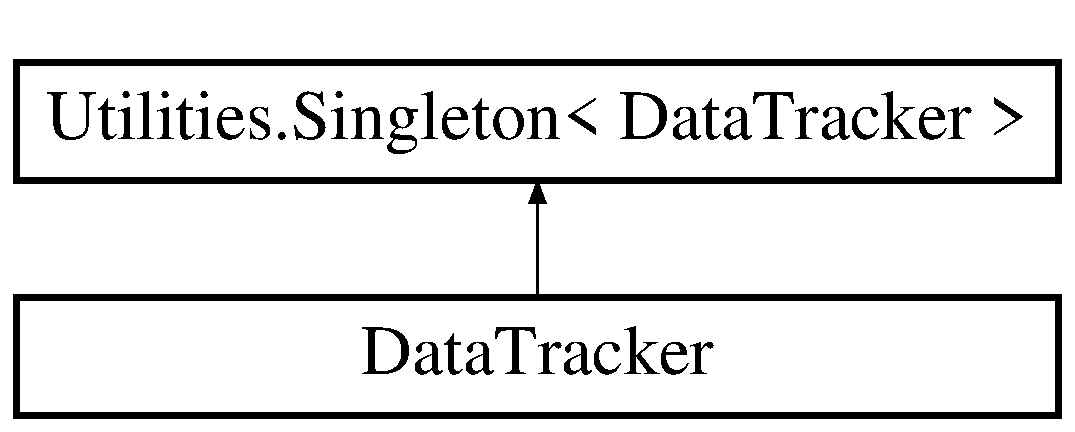
\includegraphics[height=2.000000cm]{class_data_tracker}
\end{center}
\end{figure}
\subsection*{Public Member Functions}
\begin{DoxyCompactItemize}
\item 
void \mbox{\hyperlink{class_data_tracker_a385ec3ae6529d79a33932e3c759ec2b5}{Add\+New\+Player\+Data}} (ref \mbox{\hyperlink{struct_player_data}{Player\+Data}} \+\_\+data)
\begin{DoxyCompactList}\small\item\em Adds new data to the tracked data list \end{DoxyCompactList}\item 
void \mbox{\hyperlink{class_data_tracker_ac3e1b7782c5a373f34f909549055fd6e}{Update\+Current\+Player\+Data}} (ref \mbox{\hyperlink{struct_player_data}{Player\+Data}} \+\_\+data)
\begin{DoxyCompactList}\small\item\em Update the current player data in the current playthrough data \end{DoxyCompactList}\item 
void \mbox{\hyperlink{class_data_tracker_a4869a1c8785620380fa42fef58d7ad6a}{Compare\+Player\+Data}} (\mbox{\hyperlink{struct_player_data}{Player\+Data}} \+\_\+player\+Data)
\begin{DoxyCompactList}\small\item\em Compares the current player data against the averages \end{DoxyCompactList}\item 
void \mbox{\hyperlink{class_data_tracker_ad8d42a698f0dc7bfa12d5200e158d0a4}{Add\+New\+Level\+Data}} (ref \mbox{\hyperlink{class_design_data}{Design\+Data}} \+\_\+level\+Data)
\begin{DoxyCompactList}\small\item\em Add a new level data to the playthrough data \end{DoxyCompactList}\item 
void \mbox{\hyperlink{class_data_tracker_af9257217e007188c0437f1d446542942}{Set\+Up\+Next\+Level\+Data\+And\+Send\+To\+Database}} (out int level\+Count)
\begin{DoxyCompactList}\small\item\em Create and set up a new level data struct, send old data to the database \end{DoxyCompactList}\item 
void \mbox{\hyperlink{class_data_tracker_a4b123c238cc2f165d9d12ef9c9d408d2}{Update\+Playthrough\+Data}} ()
\begin{DoxyCompactList}\small\item\em Update the playthrough data onto the database \end{DoxyCompactList}\item 
void \mbox{\hyperlink{class_data_tracker_a7b834b9df13c46f7dfa9b51e87e1c6c0}{Decide\+Next\+Difficulty}} ()
\begin{DoxyCompactList}\small\item\em Decide the next level\textquotesingle{}s difficulty \end{DoxyCompactList}\item 
Difficulty \mbox{\hyperlink{class_data_tracker_aa31f9a357bd8db7116f0070b13f673d5}{Get\+Difficulty}} ()
\begin{DoxyCompactList}\small\item\em Get the current difficulty \end{DoxyCompactList}\item 
int \mbox{\hyperlink{class_data_tracker_ac408fabd7e0e96255508610fb66a18f2}{Get\+Level\+Id}} ()
\begin{DoxyCompactList}\small\item\em Get the current playthrough ID \end{DoxyCompactList}\end{DoxyCompactItemize}
\subsection*{Protected Member Functions}
\begin{DoxyCompactItemize}
\item 
override void \mbox{\hyperlink{class_data_tracker_a683df3af0a4675dc96498519641f6c53}{Awake}} ()
\begin{DoxyCompactList}\small\item\em Initialise the data tracker object \end{DoxyCompactList}\end{DoxyCompactItemize}
\subsection*{Additional Inherited Members}


\subsection{Detailed Description}
Class to handle the data tracking over the playthrough of the demo 



Definition at line 17 of file Data\+Tracker.\+cs.



\subsection{Member Function Documentation}
\mbox{\Hypertarget{class_data_tracker_ad8d42a698f0dc7bfa12d5200e158d0a4}\label{class_data_tracker_ad8d42a698f0dc7bfa12d5200e158d0a4}} 
\index{Data\+Tracker@{Data\+Tracker}!Add\+New\+Level\+Data@{Add\+New\+Level\+Data}}
\index{Add\+New\+Level\+Data@{Add\+New\+Level\+Data}!Data\+Tracker@{Data\+Tracker}}
\subsubsection{\texorpdfstring{Add\+New\+Level\+Data()}{AddNewLevelData()}}
{\footnotesize\ttfamily void Data\+Tracker.\+Add\+New\+Level\+Data (\begin{DoxyParamCaption}\item[{ref \mbox{\hyperlink{class_design_data}{Design\+Data}}}]{\+\_\+level\+Data }\end{DoxyParamCaption})}



Add a new level data to the playthrough data 


\begin{DoxyParams}{Parameters}
{\em \+\_\+level\+Data} & Current level data\\
\hline
\end{DoxyParams}


Definition at line 385 of file Data\+Tracker.\+cs.

\mbox{\Hypertarget{class_data_tracker_a385ec3ae6529d79a33932e3c759ec2b5}\label{class_data_tracker_a385ec3ae6529d79a33932e3c759ec2b5}} 
\index{Data\+Tracker@{Data\+Tracker}!Add\+New\+Player\+Data@{Add\+New\+Player\+Data}}
\index{Add\+New\+Player\+Data@{Add\+New\+Player\+Data}!Data\+Tracker@{Data\+Tracker}}
\subsubsection{\texorpdfstring{Add\+New\+Player\+Data()}{AddNewPlayerData()}}
{\footnotesize\ttfamily void Data\+Tracker.\+Add\+New\+Player\+Data (\begin{DoxyParamCaption}\item[{ref \mbox{\hyperlink{struct_player_data}{Player\+Data}}}]{\+\_\+data }\end{DoxyParamCaption})}



Adds new data to the tracked data list 


\begin{DoxyParams}{Parameters}
{\em \+\_\+data} & Current levels player data\\
\hline
\end{DoxyParams}


Definition at line 156 of file Data\+Tracker.\+cs.

\mbox{\Hypertarget{class_data_tracker_a683df3af0a4675dc96498519641f6c53}\label{class_data_tracker_a683df3af0a4675dc96498519641f6c53}} 
\index{Data\+Tracker@{Data\+Tracker}!Awake@{Awake}}
\index{Awake@{Awake}!Data\+Tracker@{Data\+Tracker}}
\subsubsection{\texorpdfstring{Awake()}{Awake()}}
{\footnotesize\ttfamily override void Data\+Tracker.\+Awake (\begin{DoxyParamCaption}{ }\end{DoxyParamCaption})\hspace{0.3cm}{\ttfamily [protected]}, {\ttfamily [virtual]}}



Initialise the data tracker object 



Reimplemented from \mbox{\hyperlink{class_utilities_1_1_singleton_a634b915d7ac492899512de602d59e650}{Utilities.\+Singleton$<$ Data\+Tracker $>$}}.



Definition at line 64 of file Data\+Tracker.\+cs.

\mbox{\Hypertarget{class_data_tracker_a4869a1c8785620380fa42fef58d7ad6a}\label{class_data_tracker_a4869a1c8785620380fa42fef58d7ad6a}} 
\index{Data\+Tracker@{Data\+Tracker}!Compare\+Player\+Data@{Compare\+Player\+Data}}
\index{Compare\+Player\+Data@{Compare\+Player\+Data}!Data\+Tracker@{Data\+Tracker}}
\subsubsection{\texorpdfstring{Compare\+Player\+Data()}{ComparePlayerData()}}
{\footnotesize\ttfamily void Data\+Tracker.\+Compare\+Player\+Data (\begin{DoxyParamCaption}\item[{\mbox{\hyperlink{struct_player_data}{Player\+Data}}}]{\+\_\+player\+Data }\end{DoxyParamCaption})}



Compares the current player data against the averages 


\begin{DoxyParams}{Parameters}
{\em \+\_\+player\+Data} & Current levels player data\\
\hline
\end{DoxyParams}


Definition at line 179 of file Data\+Tracker.\+cs.

\mbox{\Hypertarget{class_data_tracker_a7b834b9df13c46f7dfa9b51e87e1c6c0}\label{class_data_tracker_a7b834b9df13c46f7dfa9b51e87e1c6c0}} 
\index{Data\+Tracker@{Data\+Tracker}!Decide\+Next\+Difficulty@{Decide\+Next\+Difficulty}}
\index{Decide\+Next\+Difficulty@{Decide\+Next\+Difficulty}!Data\+Tracker@{Data\+Tracker}}
\subsubsection{\texorpdfstring{Decide\+Next\+Difficulty()}{DecideNextDifficulty()}}
{\footnotesize\ttfamily void Data\+Tracker.\+Decide\+Next\+Difficulty (\begin{DoxyParamCaption}{ }\end{DoxyParamCaption})}



Decide the next level\textquotesingle{}s difficulty 



Definition at line 477 of file Data\+Tracker.\+cs.

\mbox{\Hypertarget{class_data_tracker_aa31f9a357bd8db7116f0070b13f673d5}\label{class_data_tracker_aa31f9a357bd8db7116f0070b13f673d5}} 
\index{Data\+Tracker@{Data\+Tracker}!Get\+Difficulty@{Get\+Difficulty}}
\index{Get\+Difficulty@{Get\+Difficulty}!Data\+Tracker@{Data\+Tracker}}
\subsubsection{\texorpdfstring{Get\+Difficulty()}{GetDifficulty()}}
{\footnotesize\ttfamily Difficulty Data\+Tracker.\+Get\+Difficulty (\begin{DoxyParamCaption}{ }\end{DoxyParamCaption})}



Get the current difficulty 

\begin{DoxyReturn}{Returns}
Current difficulty
\end{DoxyReturn}


Definition at line 496 of file Data\+Tracker.\+cs.

\mbox{\Hypertarget{class_data_tracker_ac408fabd7e0e96255508610fb66a18f2}\label{class_data_tracker_ac408fabd7e0e96255508610fb66a18f2}} 
\index{Data\+Tracker@{Data\+Tracker}!Get\+Level\+Id@{Get\+Level\+Id}}
\index{Get\+Level\+Id@{Get\+Level\+Id}!Data\+Tracker@{Data\+Tracker}}
\subsubsection{\texorpdfstring{Get\+Level\+Id()}{GetLevelId()}}
{\footnotesize\ttfamily int Data\+Tracker.\+Get\+Level\+Id (\begin{DoxyParamCaption}{ }\end{DoxyParamCaption})}



Get the current playthrough ID 

\begin{DoxyReturn}{Returns}
Current playthrough ID
\end{DoxyReturn}


Definition at line 505 of file Data\+Tracker.\+cs.

\mbox{\Hypertarget{class_data_tracker_af9257217e007188c0437f1d446542942}\label{class_data_tracker_af9257217e007188c0437f1d446542942}} 
\index{Data\+Tracker@{Data\+Tracker}!Set\+Up\+Next\+Level\+Data\+And\+Send\+To\+Database@{Set\+Up\+Next\+Level\+Data\+And\+Send\+To\+Database}}
\index{Set\+Up\+Next\+Level\+Data\+And\+Send\+To\+Database@{Set\+Up\+Next\+Level\+Data\+And\+Send\+To\+Database}!Data\+Tracker@{Data\+Tracker}}
\subsubsection{\texorpdfstring{Set\+Up\+Next\+Level\+Data\+And\+Send\+To\+Database()}{SetUpNextLevelDataAndSendToDatabase()}}
{\footnotesize\ttfamily void Data\+Tracker.\+Set\+Up\+Next\+Level\+Data\+And\+Send\+To\+Database (\begin{DoxyParamCaption}\item[{out int}]{level\+Count }\end{DoxyParamCaption})}



Create and set up a new level data struct, send old data to the database 


\begin{DoxyParams}{Parameters}
{\em level\+Count} & sends out the new level count\\
\hline
\end{DoxyParams}


Definition at line 395 of file Data\+Tracker.\+cs.

\mbox{\Hypertarget{class_data_tracker_ac3e1b7782c5a373f34f909549055fd6e}\label{class_data_tracker_ac3e1b7782c5a373f34f909549055fd6e}} 
\index{Data\+Tracker@{Data\+Tracker}!Update\+Current\+Player\+Data@{Update\+Current\+Player\+Data}}
\index{Update\+Current\+Player\+Data@{Update\+Current\+Player\+Data}!Data\+Tracker@{Data\+Tracker}}
\subsubsection{\texorpdfstring{Update\+Current\+Player\+Data()}{UpdateCurrentPlayerData()}}
{\footnotesize\ttfamily void Data\+Tracker.\+Update\+Current\+Player\+Data (\begin{DoxyParamCaption}\item[{ref \mbox{\hyperlink{struct_player_data}{Player\+Data}}}]{\+\_\+data }\end{DoxyParamCaption})}



Update the current player data in the current playthrough data 


\begin{DoxyParams}{Parameters}
{\em \+\_\+data} & \\
\hline
\end{DoxyParams}


Definition at line 169 of file Data\+Tracker.\+cs.

\mbox{\Hypertarget{class_data_tracker_a4b123c238cc2f165d9d12ef9c9d408d2}\label{class_data_tracker_a4b123c238cc2f165d9d12ef9c9d408d2}} 
\index{Data\+Tracker@{Data\+Tracker}!Update\+Playthrough\+Data@{Update\+Playthrough\+Data}}
\index{Update\+Playthrough\+Data@{Update\+Playthrough\+Data}!Data\+Tracker@{Data\+Tracker}}
\subsubsection{\texorpdfstring{Update\+Playthrough\+Data()}{UpdatePlaythroughData()}}
{\footnotesize\ttfamily void Data\+Tracker.\+Update\+Playthrough\+Data (\begin{DoxyParamCaption}{ }\end{DoxyParamCaption})}



Update the playthrough data onto the database 



Definition at line 420 of file Data\+Tracker.\+cs.



The documentation for this class was generated from the following file\+:\begin{DoxyCompactItemize}
\item 
C\+:/\+Users/louca/\+Documents/\+M\+A\+Dissertation/\+M\+A\+Dissertation/\+M\+A\+Dissertation/\+Assets/\+Classes/\+Database/Data\+Tracker.\+cs\end{DoxyCompactItemize}

\hypertarget{class_design_data}{}\section{Design\+Data Class Reference}
\label{class_design_data}\index{Design\+Data@{Design\+Data}}


Struct to hold all of the level\textquotesingle{}s design data  


\subsection*{Public Attributes}
\begin{DoxyCompactItemize}
\item 
\mbox{\Hypertarget{class_design_data_a882d498f174957395c3c723772a87932}\label{class_design_data_a882d498f174957395c3c723772a87932}} 
int {\bfseries m\+\_\+grid\+Width}
\item 
\mbox{\Hypertarget{class_design_data_aeaa32e60c887ac657d79a1136a984ed1}\label{class_design_data_aeaa32e60c887ac657d79a1136a984ed1}} 
int {\bfseries m\+\_\+grid\+Height}
\item 
\mbox{\Hypertarget{class_design_data_aa123d2da3927cfcea7a261e4cbf3bf35}\label{class_design_data_aa123d2da3927cfcea7a261e4cbf3bf35}} 
\mbox{\hyperlink{class_level_generation_1_1_room}{Room}} \mbox{[}$\,$\mbox{]} {\bfseries m\+\_\+grid}
\item 
\mbox{\Hypertarget{class_design_data_aed539d15f4c07a46b7314403260d8736}\label{class_design_data_aed539d15f4c07a46b7314403260d8736}} 
List$<$ \mbox{\hyperlink{struct_simple_room_data}{Simple\+Room\+Data}} $>$ {\bfseries m\+\_\+simple\+Room\+Data}
\end{DoxyCompactItemize}


\subsection{Detailed Description}
Struct to hold all of the level\textquotesingle{}s design data 



Definition at line 725 of file Data\+Tracker.\+cs.



The documentation for this class was generated from the following file\+:\begin{DoxyCompactItemize}
\item 
C\+:/\+Users/louca/\+Documents/\+M\+A\+Dissertation/\+M\+A\+Dissertation/\+M\+A\+Dissertation/\+Assets/\+Classes/\+Database/Data\+Tracker.\+cs\end{DoxyCompactItemize}

\hypertarget{class_end_zone}{}\section{End\+Zone Class Reference}
\label{class_end_zone}\index{End\+Zone@{End\+Zone}}


End of the level, triggers the next level and passing relevant data to the tracker  


Inheritance diagram for End\+Zone\+:\begin{figure}[H]
\begin{center}
\leavevmode
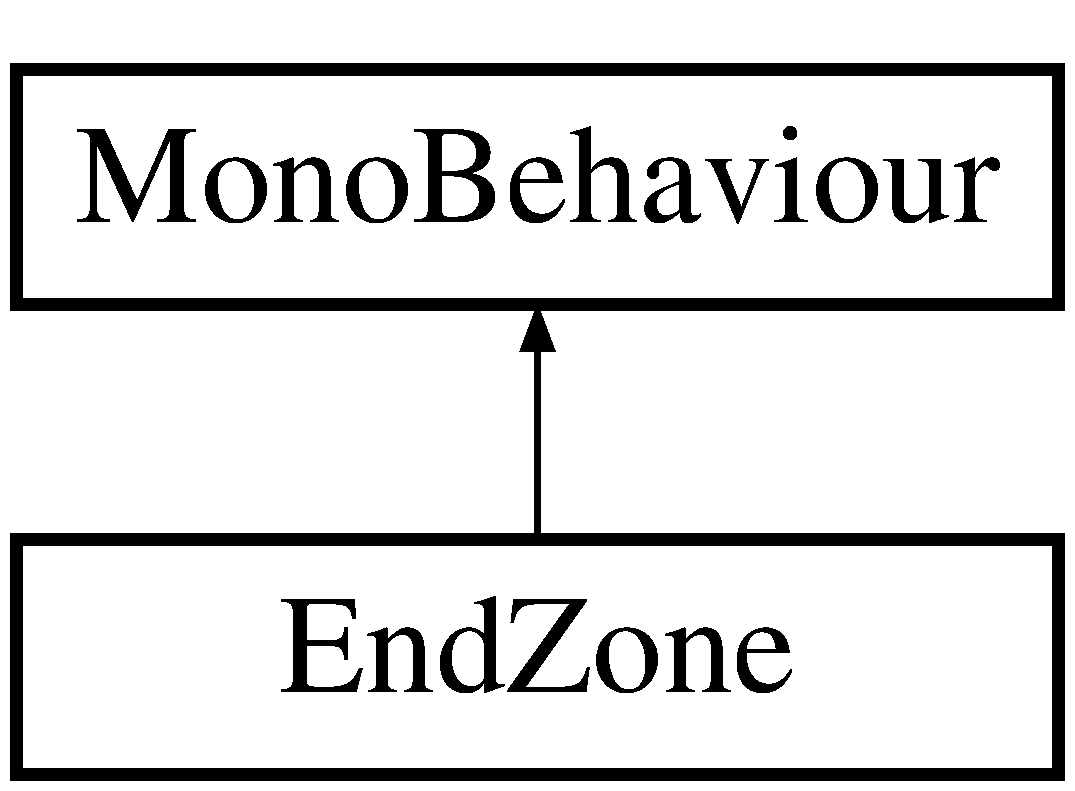
\includegraphics[height=2.000000cm]{class_end_zone}
\end{center}
\end{figure}


\subsection{Detailed Description}
End of the level, triggers the next level and passing relevant data to the tracker 



Definition at line 8 of file End\+Zone.\+cs.



The documentation for this class was generated from the following file\+:\begin{DoxyCompactItemize}
\item 
C\+:/\+Users/louca/\+Documents/\+M\+A\+Dissertation/\+M\+A\+Dissertation/\+M\+A\+Dissertation/\+Assets/\+Classes/\+Gameplay/End\+Zone.\+cs\end{DoxyCompactItemize}

\hypertarget{class_enemy}{}\section{Enemy Class Reference}
\label{class_enemy}\index{Enemy@{Enemy}}


Base enemy class  


Inheritance diagram for Enemy\+:\begin{figure}[H]
\begin{center}
\leavevmode
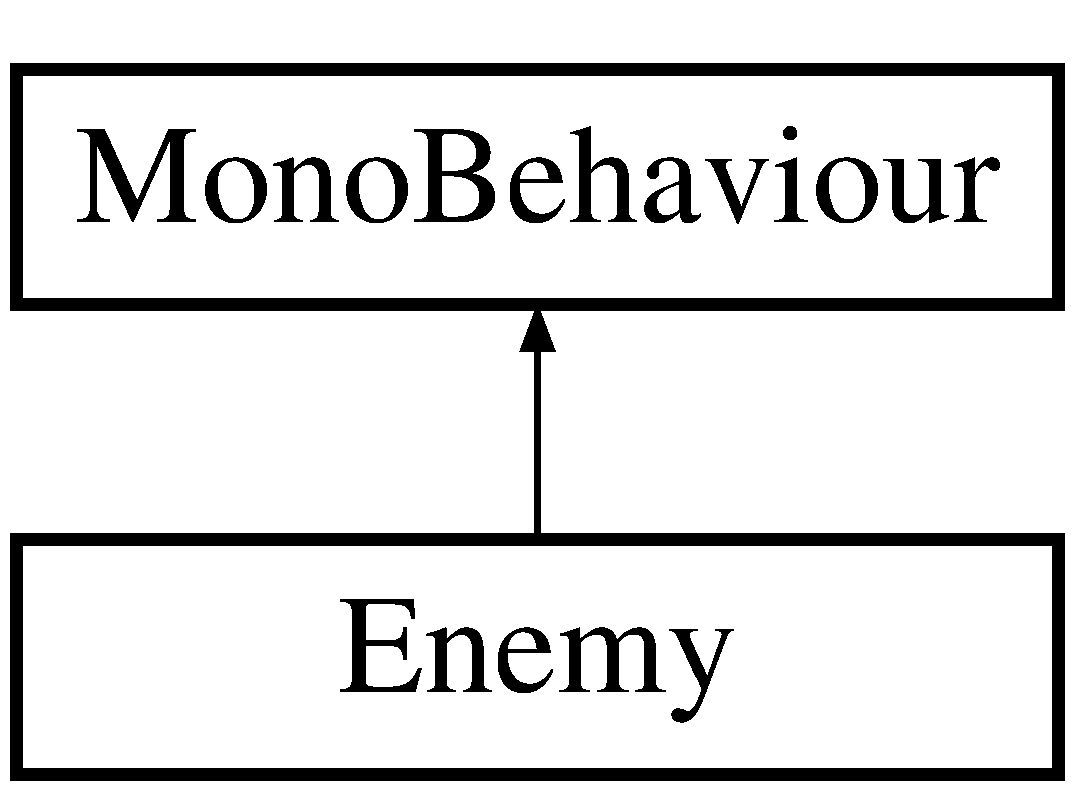
\includegraphics[height=2.000000cm]{class_enemy}
\end{center}
\end{figure}


\subsection{Detailed Description}
Base enemy class 



Definition at line 8 of file Enemy.\+cs.



The documentation for this class was generated from the following file\+:\begin{DoxyCompactItemize}
\item 
C\+:/\+Users/louca/\+Documents/\+M\+A\+Dissertation/\+M\+A\+Dissertation/\+M\+A\+Dissertation/\+Assets/\+Classes/\+Gameplay/Enemy.\+cs\end{DoxyCompactItemize}

\hypertarget{class_game_canvas}{}\section{Game\+Canvas Class Reference}
\label{class_game_canvas}\index{Game\+Canvas@{Game\+Canvas}}


A Canvas class that controls aspects of the game UI  


Inheritance diagram for Game\+Canvas\+:\begin{figure}[H]
\begin{center}
\leavevmode
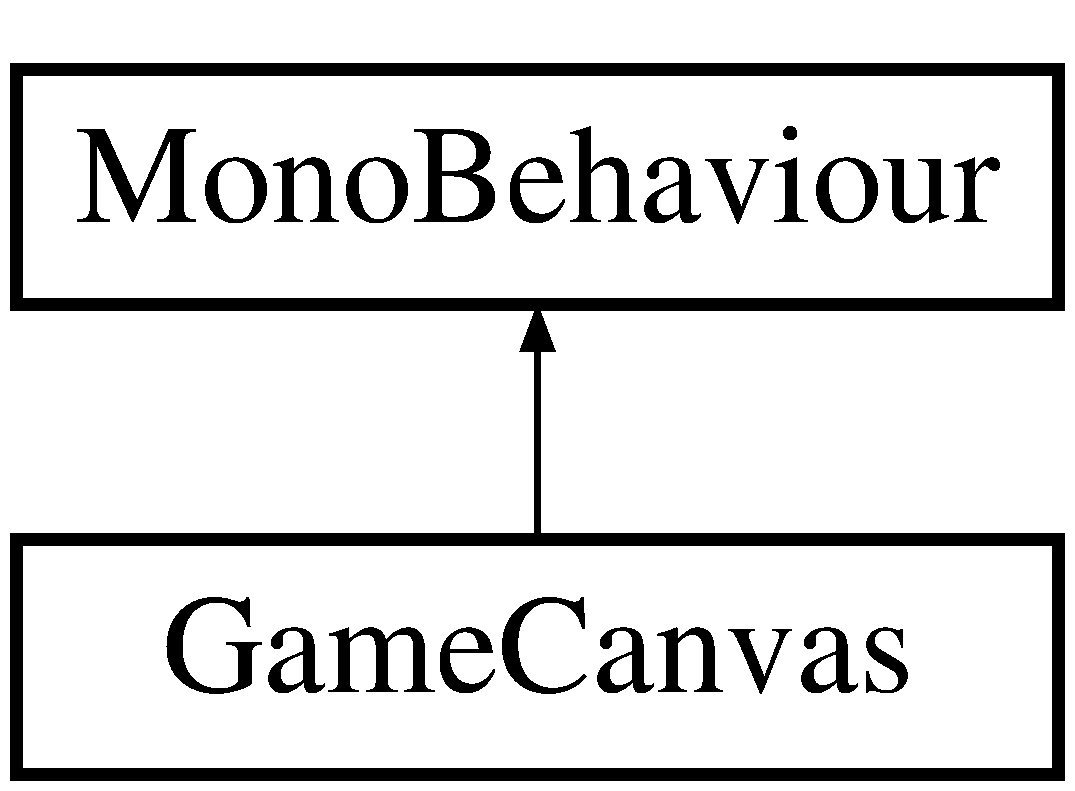
\includegraphics[height=2.000000cm]{class_game_canvas}
\end{center}
\end{figure}
\subsection*{Public Member Functions}
\begin{DoxyCompactItemize}
\item 
void \mbox{\hyperlink{class_game_canvas_a0fb4b8c30320c818ec44b62689242121}{Update\+Level\+Text}} (int \+\_\+level\+Id)
\begin{DoxyCompactList}\small\item\em Update the level text object \end{DoxyCompactList}\item 
void \mbox{\hyperlink{class_game_canvas_a1216454a399f7fd8b77126860da80802}{Update\+Deaths\+Text}} (int \+\_\+death\+Count)
\begin{DoxyCompactList}\small\item\em Update the deaths text object \end{DoxyCompactList}\item 
void \mbox{\hyperlink{class_game_canvas_a92dd51c7702d5d4e9e14902f3b31ba30}{Update\+Time\+Text}} (float \+\_\+time)
\begin{DoxyCompactList}\small\item\em Update the time text object \end{DoxyCompactList}\end{DoxyCompactItemize}


\subsection{Detailed Description}
A Canvas class that controls aspects of the game UI 



Definition at line 9 of file Game\+Canvas.\+cs.



\subsection{Member Function Documentation}
\mbox{\Hypertarget{class_game_canvas_a1216454a399f7fd8b77126860da80802}\label{class_game_canvas_a1216454a399f7fd8b77126860da80802}} 
\index{Game\+Canvas@{Game\+Canvas}!Update\+Deaths\+Text@{Update\+Deaths\+Text}}
\index{Update\+Deaths\+Text@{Update\+Deaths\+Text}!Game\+Canvas@{Game\+Canvas}}
\subsubsection{\texorpdfstring{Update\+Deaths\+Text()}{UpdateDeathsText()}}
{\footnotesize\ttfamily void Game\+Canvas.\+Update\+Deaths\+Text (\begin{DoxyParamCaption}\item[{int}]{\+\_\+death\+Count }\end{DoxyParamCaption})}



Update the deaths text object 


\begin{DoxyParams}{Parameters}
{\em \+\_\+death\+Count} & Death count value\\
\hline
\end{DoxyParams}


Definition at line 37 of file Game\+Canvas.\+cs.

\mbox{\Hypertarget{class_game_canvas_a0fb4b8c30320c818ec44b62689242121}\label{class_game_canvas_a0fb4b8c30320c818ec44b62689242121}} 
\index{Game\+Canvas@{Game\+Canvas}!Update\+Level\+Text@{Update\+Level\+Text}}
\index{Update\+Level\+Text@{Update\+Level\+Text}!Game\+Canvas@{Game\+Canvas}}
\subsubsection{\texorpdfstring{Update\+Level\+Text()}{UpdateLevelText()}}
{\footnotesize\ttfamily void Game\+Canvas.\+Update\+Level\+Text (\begin{DoxyParamCaption}\item[{int}]{\+\_\+level\+Id }\end{DoxyParamCaption})}



Update the level text object 


\begin{DoxyParams}{Parameters}
{\em \+\_\+level\+Id} & Level ID value\\
\hline
\end{DoxyParams}


Definition at line 28 of file Game\+Canvas.\+cs.

\mbox{\Hypertarget{class_game_canvas_a92dd51c7702d5d4e9e14902f3b31ba30}\label{class_game_canvas_a92dd51c7702d5d4e9e14902f3b31ba30}} 
\index{Game\+Canvas@{Game\+Canvas}!Update\+Time\+Text@{Update\+Time\+Text}}
\index{Update\+Time\+Text@{Update\+Time\+Text}!Game\+Canvas@{Game\+Canvas}}
\subsubsection{\texorpdfstring{Update\+Time\+Text()}{UpdateTimeText()}}
{\footnotesize\ttfamily void Game\+Canvas.\+Update\+Time\+Text (\begin{DoxyParamCaption}\item[{float}]{\+\_\+time }\end{DoxyParamCaption})}



Update the time text object 


\begin{DoxyParams}{Parameters}
{\em \+\_\+time} & Time value\\
\hline
\end{DoxyParams}


Definition at line 46 of file Game\+Canvas.\+cs.



The documentation for this class was generated from the following file\+:\begin{DoxyCompactItemize}
\item 
C\+:/\+Users/louca/\+Documents/\+M\+A\+Dissertation/\+M\+A\+Dissertation/\+M\+A\+Dissertation/\+Assets/\+Classes/\+U\+I/Game\+Canvas.\+cs\end{DoxyCompactItemize}

\hypertarget{class_game_manager}{}\section{Game\+Manager Class Reference}
\label{class_game_manager}\index{Game\+Manager@{Game\+Manager}}


Manages game and its states  


Inheritance diagram for Game\+Manager\+:\begin{figure}[H]
\begin{center}
\leavevmode
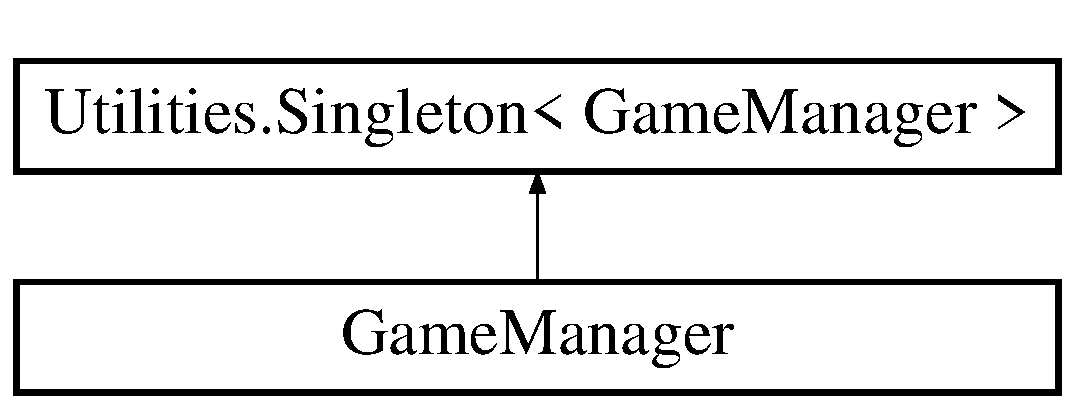
\includegraphics[height=2.000000cm]{class_game_manager}
\end{center}
\end{figure}
\subsection*{Public Member Functions}
\begin{DoxyCompactItemize}
\item 
void \mbox{\hyperlink{class_game_manager_a38cc549d56890d3d3097e0a81fd7428f}{Change\+State}} (\mbox{\hyperlink{_game_manager_8cs_a7899b65f1ea0f655e4bbf8d2a5714285}{Game\+State}} \+\_\+new\+Game\+State)
\begin{DoxyCompactList}\small\item\em Change the game state \end{DoxyCompactList}\item 
void \mbox{\hyperlink{class_game_manager_a1ba9d9459bb03a4046de5fc82734c612}{Change\+State}} (int \+\_\+new\+Game\+State)
\begin{DoxyCompactList}\small\item\em Change the game state \end{DoxyCompactList}\item 
void \mbox{\hyperlink{class_game_manager_a66796650182ecf1f1dc98c8ee889d1a0}{Update\+Current\+Level\+Lives}} (int \+\_\+lives)
\begin{DoxyCompactList}\small\item\em Update the amount of lives the player has \end{DoxyCompactList}\item 
void \mbox{\hyperlink{class_game_manager_ae77f42a6ee1bb7d5192709d24cf6ed34}{Update\+Current\+Level\+Score}} (int \+\_\+score)
\begin{DoxyCompactList}\small\item\em Update the score value \end{DoxyCompactList}\item 
\mbox{\hyperlink{_game_manager_8cs_a7899b65f1ea0f655e4bbf8d2a5714285}{Game\+State}} \mbox{\hyperlink{class_game_manager_a58134230a7cde001ebf2b25f1dcd6091}{Get\+Game\+State}} ()
\begin{DoxyCompactList}\small\item\em Allow other classes access to the current game state \end{DoxyCompactList}\item 
bool \mbox{\hyperlink{class_game_manager_a35822d3c950f5d43e34c2f020d46c23d}{Is\+Debug}} ()
\begin{DoxyCompactList}\small\item\em Allows other classes to see if the game is in debug mode \end{DoxyCompactList}\item 
void \mbox{\hyperlink{class_game_manager_a8778b6ae7b19b87aff284883c2bda04a}{Update\+Data\+On\+Database}} ()
\end{DoxyCompactItemize}
\subsection*{Private Member Functions}
\begin{DoxyCompactItemize}
\item 
void \mbox{\hyperlink{class_game_manager_a5ccfacd027ad08eeb4ff1f25a7f59c98}{Start}} ()
\item 
void \mbox{\hyperlink{class_game_manager_a44c79b205dec16bfe650e21259860c5b}{Update}} ()
\item 
I\+Enumerator \mbox{\hyperlink{class_game_manager_a5b92f7fbdd78acc3576b9f8fa83a7f6b}{Load\+Next\+Level}} ()
\begin{DoxyCompactList}\small\item\em Loads the next level \end{DoxyCompactList}\item 
I\+Enumerator \mbox{\hyperlink{class_game_manager_a5c23fa91837ebfc3f114e315ee4a0623}{Load\+Main\+Menu}} ()
\begin{DoxyCompactList}\small\item\em Loads the main menu scene \end{DoxyCompactList}\item 
I\+Enumerator \mbox{\hyperlink{class_game_manager_a4d01c563f63394c879c458b8449967a0}{Reset\+After\+Game\+Over}} ()
\begin{DoxyCompactList}\small\item\em Reset the game after the player dies \end{DoxyCompactList}\end{DoxyCompactItemize}
\subsection*{Private Attributes}
\begin{DoxyCompactItemize}
\item 
Game\+Object \mbox{\hyperlink{class_game_manager_afe830d016f2ae2f5b74e792bcd957cb4}{m\+\_\+scene\+Loader\+Prefab}}
\item 
bool \mbox{\hyperlink{class_game_manager_a7aed1c66e288d6712e7b04c12bd0d5cc}{m\+\_\+debug\+Mode}} = false
\item 
int \mbox{\hyperlink{class_game_manager_a8166d596fca625618a2b5ab261b07659}{m\+\_\+level\+Limit}} = 10
\item 
\mbox{\hyperlink{_game_manager_8cs_a7899b65f1ea0f655e4bbf8d2a5714285}{Game\+State}} \mbox{\hyperlink{class_game_manager_a17e003b42eb6c99308a04813e359ff71}{m\+\_\+game\+State}} = \mbox{\hyperlink{_game_manager_8cs_a7899b65f1ea0f655e4bbf8d2a5714285a95b19f7739b0b7ea7d6b07586be54f36}{Game\+State.\+Init}}
\item 
Game\+Object \mbox{\hyperlink{class_game_manager_a0fed6d237d49a6a342b35a4423e6c03d}{m\+\_\+respawning\+Text}}
\item 
Player\+Data \mbox{\hyperlink{class_game_manager_a8e671c2fc013be135ec70b43aea3a29e}{m\+\_\+current\+Player\+Data}}
\item 
Canvas\+Manager \mbox{\hyperlink{class_game_manager_ad3abeb539c4f257789aa7134c752c786}{m\+\_\+canvas\+Manager}} = null
\end{DoxyCompactItemize}


\subsection{Detailed Description}
Manages game and its states 



Definition at line 9 of file Game\+Manager.\+cs.



\subsection{Member Function Documentation}
\mbox{\Hypertarget{class_game_manager_a38cc549d56890d3d3097e0a81fd7428f}\label{class_game_manager_a38cc549d56890d3d3097e0a81fd7428f}} 
\index{Game\+Manager@{Game\+Manager}!Change\+State@{Change\+State}}
\index{Change\+State@{Change\+State}!Game\+Manager@{Game\+Manager}}
\subsubsection{\texorpdfstring{Change\+State()}{ChangeState()}\hspace{0.1cm}{\footnotesize\ttfamily [1/2]}}
{\footnotesize\ttfamily void Game\+Manager.\+Change\+State (\begin{DoxyParamCaption}\item[{\mbox{\hyperlink{_game_manager_8cs_a7899b65f1ea0f655e4bbf8d2a5714285}{Game\+State}}}]{\+\_\+new\+Game\+State }\end{DoxyParamCaption})}



Change the game state 


\begin{DoxyParams}{Parameters}
{\em \+\_\+new\+Game\+State} & New game state\\
\hline
\end{DoxyParams}


Definition at line 90 of file Game\+Manager.\+cs.

\mbox{\Hypertarget{class_game_manager_a1ba9d9459bb03a4046de5fc82734c612}\label{class_game_manager_a1ba9d9459bb03a4046de5fc82734c612}} 
\index{Game\+Manager@{Game\+Manager}!Change\+State@{Change\+State}}
\index{Change\+State@{Change\+State}!Game\+Manager@{Game\+Manager}}
\subsubsection{\texorpdfstring{Change\+State()}{ChangeState()}\hspace{0.1cm}{\footnotesize\ttfamily [2/2]}}
{\footnotesize\ttfamily void Game\+Manager.\+Change\+State (\begin{DoxyParamCaption}\item[{int}]{\+\_\+new\+Game\+State }\end{DoxyParamCaption})}



Change the game state 


\begin{DoxyParams}{Parameters}
{\em \+\_\+new\+Game\+State} & New game state\\
\hline
\end{DoxyParams}


Definition at line 285 of file Game\+Manager.\+cs.

\mbox{\Hypertarget{class_game_manager_a58134230a7cde001ebf2b25f1dcd6091}\label{class_game_manager_a58134230a7cde001ebf2b25f1dcd6091}} 
\index{Game\+Manager@{Game\+Manager}!Get\+Game\+State@{Get\+Game\+State}}
\index{Get\+Game\+State@{Get\+Game\+State}!Game\+Manager@{Game\+Manager}}
\subsubsection{\texorpdfstring{Get\+Game\+State()}{GetGameState()}}
{\footnotesize\ttfamily \mbox{\hyperlink{_game_manager_8cs_a7899b65f1ea0f655e4bbf8d2a5714285}{Game\+State}} Game\+Manager.\+Get\+Game\+State (\begin{DoxyParamCaption}{ }\end{DoxyParamCaption})}



Allow other classes access to the current game state 

\begin{DoxyReturn}{Returns}
Returns the current game state
\end{DoxyReturn}


Definition at line 398 of file Game\+Manager.\+cs.

\mbox{\Hypertarget{class_game_manager_a35822d3c950f5d43e34c2f020d46c23d}\label{class_game_manager_a35822d3c950f5d43e34c2f020d46c23d}} 
\index{Game\+Manager@{Game\+Manager}!Is\+Debug@{Is\+Debug}}
\index{Is\+Debug@{Is\+Debug}!Game\+Manager@{Game\+Manager}}
\subsubsection{\texorpdfstring{Is\+Debug()}{IsDebug()}}
{\footnotesize\ttfamily bool Game\+Manager.\+Is\+Debug (\begin{DoxyParamCaption}{ }\end{DoxyParamCaption})}



Allows other classes to see if the game is in debug mode 

\begin{DoxyReturn}{Returns}
Returns true if the game is in debug mode but false if not
\end{DoxyReturn}


Definition at line 407 of file Game\+Manager.\+cs.

\mbox{\Hypertarget{class_game_manager_a5c23fa91837ebfc3f114e315ee4a0623}\label{class_game_manager_a5c23fa91837ebfc3f114e315ee4a0623}} 
\index{Game\+Manager@{Game\+Manager}!Load\+Main\+Menu@{Load\+Main\+Menu}}
\index{Load\+Main\+Menu@{Load\+Main\+Menu}!Game\+Manager@{Game\+Manager}}
\subsubsection{\texorpdfstring{Load\+Main\+Menu()}{LoadMainMenu()}}
{\footnotesize\ttfamily I\+Enumerator Game\+Manager.\+Load\+Main\+Menu (\begin{DoxyParamCaption}{ }\end{DoxyParamCaption})\hspace{0.3cm}{\ttfamily [private]}}



Loads the main menu scene 

\begin{DoxyReturn}{Returns}

\end{DoxyReturn}


Definition at line 272 of file Game\+Manager.\+cs.

\mbox{\Hypertarget{class_game_manager_a5b92f7fbdd78acc3576b9f8fa83a7f6b}\label{class_game_manager_a5b92f7fbdd78acc3576b9f8fa83a7f6b}} 
\index{Game\+Manager@{Game\+Manager}!Load\+Next\+Level@{Load\+Next\+Level}}
\index{Load\+Next\+Level@{Load\+Next\+Level}!Game\+Manager@{Game\+Manager}}
\subsubsection{\texorpdfstring{Load\+Next\+Level()}{LoadNextLevel()}}
{\footnotesize\ttfamily I\+Enumerator Game\+Manager.\+Load\+Next\+Level (\begin{DoxyParamCaption}{ }\end{DoxyParamCaption})\hspace{0.3cm}{\ttfamily [private]}}



Loads the next level 

\begin{DoxyReturn}{Returns}

\end{DoxyReturn}


Definition at line 256 of file Game\+Manager.\+cs.

\mbox{\Hypertarget{class_game_manager_a4d01c563f63394c879c458b8449967a0}\label{class_game_manager_a4d01c563f63394c879c458b8449967a0}} 
\index{Game\+Manager@{Game\+Manager}!Reset\+After\+Game\+Over@{Reset\+After\+Game\+Over}}
\index{Reset\+After\+Game\+Over@{Reset\+After\+Game\+Over}!Game\+Manager@{Game\+Manager}}
\subsubsection{\texorpdfstring{Reset\+After\+Game\+Over()}{ResetAfterGameOver()}}
{\footnotesize\ttfamily I\+Enumerator Game\+Manager.\+Reset\+After\+Game\+Over (\begin{DoxyParamCaption}{ }\end{DoxyParamCaption})\hspace{0.3cm}{\ttfamily [private]}}



Reset the game after the player dies 

\begin{DoxyReturn}{Returns}

\end{DoxyReturn}


Definition at line 367 of file Game\+Manager.\+cs.

\mbox{\Hypertarget{class_game_manager_a5ccfacd027ad08eeb4ff1f25a7f59c98}\label{class_game_manager_a5ccfacd027ad08eeb4ff1f25a7f59c98}} 
\index{Game\+Manager@{Game\+Manager}!Start@{Start}}
\index{Start@{Start}!Game\+Manager@{Game\+Manager}}
\subsubsection{\texorpdfstring{Start()}{Start()}}
{\footnotesize\ttfamily void Game\+Manager.\+Start (\begin{DoxyParamCaption}{ }\end{DoxyParamCaption})\hspace{0.3cm}{\ttfamily [private]}}



Definition at line 28 of file Game\+Manager.\+cs.

\mbox{\Hypertarget{class_game_manager_a44c79b205dec16bfe650e21259860c5b}\label{class_game_manager_a44c79b205dec16bfe650e21259860c5b}} 
\index{Game\+Manager@{Game\+Manager}!Update@{Update}}
\index{Update@{Update}!Game\+Manager@{Game\+Manager}}
\subsubsection{\texorpdfstring{Update()}{Update()}}
{\footnotesize\ttfamily void Game\+Manager.\+Update (\begin{DoxyParamCaption}{ }\end{DoxyParamCaption})\hspace{0.3cm}{\ttfamily [private]}}



Definition at line 35 of file Game\+Manager.\+cs.

\mbox{\Hypertarget{class_game_manager_a66796650182ecf1f1dc98c8ee889d1a0}\label{class_game_manager_a66796650182ecf1f1dc98c8ee889d1a0}} 
\index{Game\+Manager@{Game\+Manager}!Update\+Current\+Level\+Lives@{Update\+Current\+Level\+Lives}}
\index{Update\+Current\+Level\+Lives@{Update\+Current\+Level\+Lives}!Game\+Manager@{Game\+Manager}}
\subsubsection{\texorpdfstring{Update\+Current\+Level\+Lives()}{UpdateCurrentLevelLives()}}
{\footnotesize\ttfamily void Game\+Manager.\+Update\+Current\+Level\+Lives (\begin{DoxyParamCaption}\item[{int}]{\+\_\+lives }\end{DoxyParamCaption})}



Update the amount of lives the player has 


\begin{DoxyParams}{Parameters}
{\em \+\_\+lives} & Lives value\\
\hline
\end{DoxyParams}


Definition at line 380 of file Game\+Manager.\+cs.

\mbox{\Hypertarget{class_game_manager_ae77f42a6ee1bb7d5192709d24cf6ed34}\label{class_game_manager_ae77f42a6ee1bb7d5192709d24cf6ed34}} 
\index{Game\+Manager@{Game\+Manager}!Update\+Current\+Level\+Score@{Update\+Current\+Level\+Score}}
\index{Update\+Current\+Level\+Score@{Update\+Current\+Level\+Score}!Game\+Manager@{Game\+Manager}}
\subsubsection{\texorpdfstring{Update\+Current\+Level\+Score()}{UpdateCurrentLevelScore()}}
{\footnotesize\ttfamily void Game\+Manager.\+Update\+Current\+Level\+Score (\begin{DoxyParamCaption}\item[{int}]{\+\_\+score }\end{DoxyParamCaption})}



Update the score value 


\begin{DoxyParams}{Parameters}
{\em \+\_\+score} & Score value\\
\hline
\end{DoxyParams}


Definition at line 389 of file Game\+Manager.\+cs.

\mbox{\Hypertarget{class_game_manager_a8778b6ae7b19b87aff284883c2bda04a}\label{class_game_manager_a8778b6ae7b19b87aff284883c2bda04a}} 
\index{Game\+Manager@{Game\+Manager}!Update\+Data\+On\+Database@{Update\+Data\+On\+Database}}
\index{Update\+Data\+On\+Database@{Update\+Data\+On\+Database}!Game\+Manager@{Game\+Manager}}
\subsubsection{\texorpdfstring{Update\+Data\+On\+Database()}{UpdateDataOnDatabase()}}
{\footnotesize\ttfamily void Game\+Manager.\+Update\+Data\+On\+Database (\begin{DoxyParamCaption}{ }\end{DoxyParamCaption})}



Definition at line 412 of file Game\+Manager.\+cs.



\subsection{Member Data Documentation}
\mbox{\Hypertarget{class_game_manager_ad3abeb539c4f257789aa7134c752c786}\label{class_game_manager_ad3abeb539c4f257789aa7134c752c786}} 
\index{Game\+Manager@{Game\+Manager}!m\+\_\+canvas\+Manager@{m\+\_\+canvas\+Manager}}
\index{m\+\_\+canvas\+Manager@{m\+\_\+canvas\+Manager}!Game\+Manager@{Game\+Manager}}
\subsubsection{\texorpdfstring{m\+\_\+canvas\+Manager}{m\_canvasManager}}
{\footnotesize\ttfamily Canvas\+Manager Game\+Manager.\+m\+\_\+canvas\+Manager = null\hspace{0.3cm}{\ttfamily [private]}}



Definition at line 25 of file Game\+Manager.\+cs.

\mbox{\Hypertarget{class_game_manager_a8e671c2fc013be135ec70b43aea3a29e}\label{class_game_manager_a8e671c2fc013be135ec70b43aea3a29e}} 
\index{Game\+Manager@{Game\+Manager}!m\+\_\+current\+Player\+Data@{m\+\_\+current\+Player\+Data}}
\index{m\+\_\+current\+Player\+Data@{m\+\_\+current\+Player\+Data}!Game\+Manager@{Game\+Manager}}
\subsubsection{\texorpdfstring{m\+\_\+current\+Player\+Data}{m\_currentPlayerData}}
{\footnotesize\ttfamily Player\+Data Game\+Manager.\+m\+\_\+current\+Player\+Data\hspace{0.3cm}{\ttfamily [private]}}



Definition at line 24 of file Game\+Manager.\+cs.

\mbox{\Hypertarget{class_game_manager_a7aed1c66e288d6712e7b04c12bd0d5cc}\label{class_game_manager_a7aed1c66e288d6712e7b04c12bd0d5cc}} 
\index{Game\+Manager@{Game\+Manager}!m\+\_\+debug\+Mode@{m\+\_\+debug\+Mode}}
\index{m\+\_\+debug\+Mode@{m\+\_\+debug\+Mode}!Game\+Manager@{Game\+Manager}}
\subsubsection{\texorpdfstring{m\+\_\+debug\+Mode}{m\_debugMode}}
{\footnotesize\ttfamily bool Game\+Manager.\+m\+\_\+debug\+Mode = false\hspace{0.3cm}{\ttfamily [private]}}



Definition at line 16 of file Game\+Manager.\+cs.

\mbox{\Hypertarget{class_game_manager_a17e003b42eb6c99308a04813e359ff71}\label{class_game_manager_a17e003b42eb6c99308a04813e359ff71}} 
\index{Game\+Manager@{Game\+Manager}!m\+\_\+game\+State@{m\+\_\+game\+State}}
\index{m\+\_\+game\+State@{m\+\_\+game\+State}!Game\+Manager@{Game\+Manager}}
\subsubsection{\texorpdfstring{m\+\_\+game\+State}{m\_gameState}}
{\footnotesize\ttfamily \mbox{\hyperlink{_game_manager_8cs_a7899b65f1ea0f655e4bbf8d2a5714285}{Game\+State}} Game\+Manager.\+m\+\_\+game\+State = \mbox{\hyperlink{_game_manager_8cs_a7899b65f1ea0f655e4bbf8d2a5714285a95b19f7739b0b7ea7d6b07586be54f36}{Game\+State.\+Init}}\hspace{0.3cm}{\ttfamily [private]}}



Definition at line 22 of file Game\+Manager.\+cs.

\mbox{\Hypertarget{class_game_manager_a8166d596fca625618a2b5ab261b07659}\label{class_game_manager_a8166d596fca625618a2b5ab261b07659}} 
\index{Game\+Manager@{Game\+Manager}!m\+\_\+level\+Limit@{m\+\_\+level\+Limit}}
\index{m\+\_\+level\+Limit@{m\+\_\+level\+Limit}!Game\+Manager@{Game\+Manager}}
\subsubsection{\texorpdfstring{m\+\_\+level\+Limit}{m\_levelLimit}}
{\footnotesize\ttfamily int Game\+Manager.\+m\+\_\+level\+Limit = 10\hspace{0.3cm}{\ttfamily [private]}}



Definition at line 19 of file Game\+Manager.\+cs.

\mbox{\Hypertarget{class_game_manager_a0fed6d237d49a6a342b35a4423e6c03d}\label{class_game_manager_a0fed6d237d49a6a342b35a4423e6c03d}} 
\index{Game\+Manager@{Game\+Manager}!m\+\_\+respawning\+Text@{m\+\_\+respawning\+Text}}
\index{m\+\_\+respawning\+Text@{m\+\_\+respawning\+Text}!Game\+Manager@{Game\+Manager}}
\subsubsection{\texorpdfstring{m\+\_\+respawning\+Text}{m\_respawningText}}
{\footnotesize\ttfamily Game\+Object Game\+Manager.\+m\+\_\+respawning\+Text\hspace{0.3cm}{\ttfamily [private]}}



Definition at line 23 of file Game\+Manager.\+cs.

\mbox{\Hypertarget{class_game_manager_afe830d016f2ae2f5b74e792bcd957cb4}\label{class_game_manager_afe830d016f2ae2f5b74e792bcd957cb4}} 
\index{Game\+Manager@{Game\+Manager}!m\+\_\+scene\+Loader\+Prefab@{m\+\_\+scene\+Loader\+Prefab}}
\index{m\+\_\+scene\+Loader\+Prefab@{m\+\_\+scene\+Loader\+Prefab}!Game\+Manager@{Game\+Manager}}
\subsubsection{\texorpdfstring{m\+\_\+scene\+Loader\+Prefab}{m\_sceneLoaderPrefab}}
{\footnotesize\ttfamily Game\+Object Game\+Manager.\+m\+\_\+scene\+Loader\+Prefab\hspace{0.3cm}{\ttfamily [private]}}



Definition at line 13 of file Game\+Manager.\+cs.



The documentation for this class was generated from the following file\+:\begin{DoxyCompactItemize}
\item 
C\+:/\+Users/louca/\+Documents/\+M\+A\+Dissertation/\+M\+A\+Dissertation/\+M\+A\+Dissertation/\+Assets/\+Classes/\mbox{\hyperlink{_game_manager_8cs}{Game\+Manager.\+cs}}\end{DoxyCompactItemize}

\hypertarget{class_level_generation_1_1_grid}{}\section{Level\+Generation.\+Grid Class Reference}
\label{class_level_generation_1_1_grid}\index{Level\+Generation.\+Grid@{Level\+Generation.\+Grid}}


\mbox{\hyperlink{class_level_generation_1_1_grid}{Grid}} class that is used to generate the levels  


Inheritance diagram for Level\+Generation.\+Grid\+:\begin{figure}[H]
\begin{center}
\leavevmode
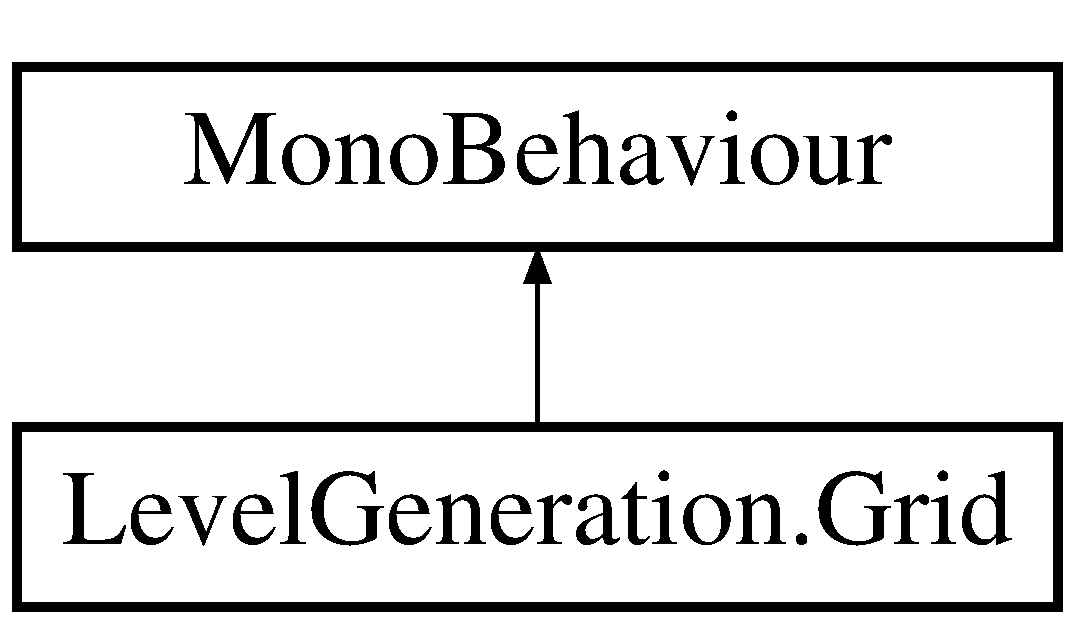
\includegraphics[height=2.000000cm]{class_level_generation_1_1_grid}
\end{center}
\end{figure}
\subsection*{Public Member Functions}
\begin{DoxyCompactItemize}
\item 
void \mbox{\hyperlink{class_level_generation_1_1_grid_aafba1625abf1acd433a19d7b82c00ae2}{Create\+Grid}} (int \+\_\+grid\+Width, int \+\_\+grid\+Height, Game\+Object \+\_\+empty\+Room, Vector2 \+\_\+offset, \mbox{\hyperlink{class_level_generation_1_1_template_holder}{Template\+Holder}} \+\_\+template\+Holder, \mbox{\hyperlink{class_camera_movement}{Camera\+Movement}} \+\_\+camera\+Movement, Game\+Object \+\_\+player)
\begin{DoxyCompactList}\small\item\em Create a grid of empty rooms \end{DoxyCompactList}\item 
void \mbox{\hyperlink{class_level_generation_1_1_grid_aa69c03ea0068b2254d58d47615f67a80}{Generate\+Level}} ()
\begin{DoxyCompactList}\small\item\em Generate a level \end{DoxyCompactList}\item 
\mbox{\hyperlink{class_level_generation_1_1_room}{Room}} \mbox{\hyperlink{class_level_generation_1_1_grid_a82ed4d13492ff553b3a20388f96fb0f3}{Get\+Room}} (int \+\_\+x, int \+\_\+y)
\begin{DoxyCompactList}\small\item\em Get a specific room \end{DoxyCompactList}\item 
void \mbox{\hyperlink{class_level_generation_1_1_grid_a7ff44c0b5eeb4cc035b35f244089f33d}{Clear}} ()
\begin{DoxyCompactList}\small\item\em Clear the grid \end{DoxyCompactList}\end{DoxyCompactItemize}


\subsection{Detailed Description}
\mbox{\hyperlink{class_level_generation_1_1_grid}{Grid}} class that is used to generate the levels 



Definition at line 15 of file Grid.\+cs.



\subsection{Member Function Documentation}
\mbox{\Hypertarget{class_level_generation_1_1_grid_a7ff44c0b5eeb4cc035b35f244089f33d}\label{class_level_generation_1_1_grid_a7ff44c0b5eeb4cc035b35f244089f33d}} 
\index{Level\+Generation\+::\+Grid@{Level\+Generation\+::\+Grid}!Clear@{Clear}}
\index{Clear@{Clear}!Level\+Generation\+::\+Grid@{Level\+Generation\+::\+Grid}}
\subsubsection{\texorpdfstring{Clear()}{Clear()}}
{\footnotesize\ttfamily void Level\+Generation.\+Grid.\+Clear (\begin{DoxyParamCaption}{ }\end{DoxyParamCaption})}



Clear the grid 



Definition at line 461 of file Grid.\+cs.

\mbox{\Hypertarget{class_level_generation_1_1_grid_aafba1625abf1acd433a19d7b82c00ae2}\label{class_level_generation_1_1_grid_aafba1625abf1acd433a19d7b82c00ae2}} 
\index{Level\+Generation\+::\+Grid@{Level\+Generation\+::\+Grid}!Create\+Grid@{Create\+Grid}}
\index{Create\+Grid@{Create\+Grid}!Level\+Generation\+::\+Grid@{Level\+Generation\+::\+Grid}}
\subsubsection{\texorpdfstring{Create\+Grid()}{CreateGrid()}}
{\footnotesize\ttfamily void Level\+Generation.\+Grid.\+Create\+Grid (\begin{DoxyParamCaption}\item[{int}]{\+\_\+grid\+Width,  }\item[{int}]{\+\_\+grid\+Height,  }\item[{Game\+Object}]{\+\_\+empty\+Room,  }\item[{Vector2}]{\+\_\+offset,  }\item[{\mbox{\hyperlink{class_level_generation_1_1_template_holder}{Template\+Holder}}}]{\+\_\+template\+Holder,  }\item[{\mbox{\hyperlink{class_camera_movement}{Camera\+Movement}}}]{\+\_\+camera\+Movement,  }\item[{Game\+Object}]{\+\_\+player }\end{DoxyParamCaption})}



Create a grid of empty rooms 


\begin{DoxyParams}{Parameters}
{\em \+\_\+grid\+Width} & \mbox{\hyperlink{class_level_generation_1_1_grid}{Grid}} Width\\
\hline
{\em \+\_\+grid\+Height} & \mbox{\hyperlink{class_level_generation_1_1_grid}{Grid}} Height\\
\hline
{\em \+\_\+empty\+Room} & Empty \mbox{\hyperlink{class_level_generation_1_1_room}{Room}} Prefab\\
\hline
{\em \+\_\+offset} & Position Offset\\
\hline
{\em \+\_\+template\+Holder} & Template Holder Scriptable Object\\
\hline
{\em \+\_\+camera\+Movement} & Camera Movement Class\\
\hline
{\em \+\_\+player} & \mbox{\hyperlink{class_player}{Player}} Prefab\\
\hline
\end{DoxyParams}


Definition at line 38 of file Grid.\+cs.

\mbox{\Hypertarget{class_level_generation_1_1_grid_aa69c03ea0068b2254d58d47615f67a80}\label{class_level_generation_1_1_grid_aa69c03ea0068b2254d58d47615f67a80}} 
\index{Level\+Generation\+::\+Grid@{Level\+Generation\+::\+Grid}!Generate\+Level@{Generate\+Level}}
\index{Generate\+Level@{Generate\+Level}!Level\+Generation\+::\+Grid@{Level\+Generation\+::\+Grid}}
\subsubsection{\texorpdfstring{Generate\+Level()}{GenerateLevel()}}
{\footnotesize\ttfamily void Level\+Generation.\+Grid.\+Generate\+Level (\begin{DoxyParamCaption}{ }\end{DoxyParamCaption})}



Generate a level 



Definition at line 98 of file Grid.\+cs.

\mbox{\Hypertarget{class_level_generation_1_1_grid_a82ed4d13492ff553b3a20388f96fb0f3}\label{class_level_generation_1_1_grid_a82ed4d13492ff553b3a20388f96fb0f3}} 
\index{Level\+Generation\+::\+Grid@{Level\+Generation\+::\+Grid}!Get\+Room@{Get\+Room}}
\index{Get\+Room@{Get\+Room}!Level\+Generation\+::\+Grid@{Level\+Generation\+::\+Grid}}
\subsubsection{\texorpdfstring{Get\+Room()}{GetRoom()}}
{\footnotesize\ttfamily \mbox{\hyperlink{class_level_generation_1_1_room}{Room}} Level\+Generation.\+Grid.\+Get\+Room (\begin{DoxyParamCaption}\item[{int}]{\+\_\+x,  }\item[{int}]{\+\_\+y }\end{DoxyParamCaption})}



Get a specific room 


\begin{DoxyParams}{Parameters}
{\em \+\_\+x} & X position\\
\hline
{\em \+\_\+y} & Y position\\
\hline
\end{DoxyParams}
\begin{DoxyReturn}{Returns}
\mbox{\hyperlink{class_level_generation_1_1_room}{Room}} matching the specific co ordinates
\end{DoxyReturn}


Definition at line 453 of file Grid.\+cs.



The documentation for this class was generated from the following file\+:\begin{DoxyCompactItemize}
\item 
C\+:/\+Users/louca/\+Documents/\+M\+A\+Dissertation/\+M\+A\+Dissertation/\+M\+A\+Dissertation/\+Assets/\+Classes/\+Level Generator/Grid.\+cs\end{DoxyCompactItemize}

\hypertarget{class_grinder_obstacle}{}\section{Grinder\+Obstacle Class Reference}
\label{class_grinder_obstacle}\index{Grinder\+Obstacle@{Grinder\+Obstacle}}


A Grinder obstacle that the player has to avoid  


Inheritance diagram for Grinder\+Obstacle\+:\begin{figure}[H]
\begin{center}
\leavevmode
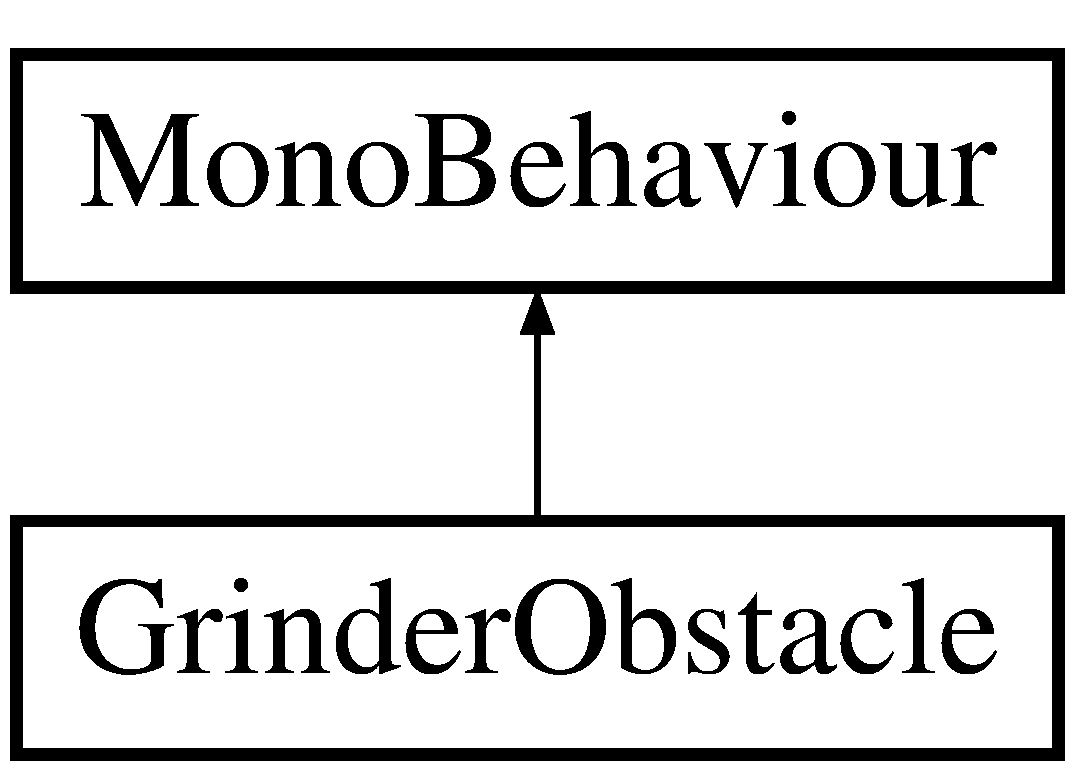
\includegraphics[height=2.000000cm]{class_grinder_obstacle}
\end{center}
\end{figure}


\subsection{Detailed Description}
A Grinder obstacle that the player has to avoid 



Definition at line 8 of file Grinder\+Obstacle.\+cs.



The documentation for this class was generated from the following file\+:\begin{DoxyCompactItemize}
\item 
C\+:/\+Users/louca/\+Documents/\+M\+A\+Dissertation/\+M\+A\+Dissertation/\+M\+A\+Dissertation/\+Assets/\+Classes/\+Gameplay/Grinder\+Obstacle.\+cs\end{DoxyCompactItemize}

\hypertarget{struct_input_scheme_objects}{}\section{Input\+Scheme\+Objects Struct Reference}
\label{struct_input_scheme_objects}\index{Input\+Scheme\+Objects@{Input\+Scheme\+Objects}}


A struct containing the input name and various input text objects  


\subsection*{Public Attributes}
\begin{DoxyCompactItemize}
\item 
\mbox{\Hypertarget{struct_input_scheme_objects_ab904862cde384666bb13ae949342558c}\label{struct_input_scheme_objects_ab904862cde384666bb13ae949342558c}} 
string {\bfseries m\+\_\+name}
\item 
\mbox{\Hypertarget{struct_input_scheme_objects_a0cfd3f09491b08a21eea814892d7285c}\label{struct_input_scheme_objects_a0cfd3f09491b08a21eea814892d7285c}} 
Game\+Object {\bfseries m\+\_\+gameplay\+Input}
\item 
\mbox{\Hypertarget{struct_input_scheme_objects_a35e337752b476d47a19e4984b470c5af}\label{struct_input_scheme_objects_a35e337752b476d47a19e4984b470c5af}} 
Game\+Object {\bfseries m\+\_\+ui\+Input}
\end{DoxyCompactItemize}


\subsection{Detailed Description}
A struct containing the input name and various input text objects 



Definition at line 223 of file Control\+Scheme.\+cs.



The documentation for this struct was generated from the following file\+:\begin{DoxyCompactItemize}
\item 
C\+:/\+Users/louca/\+Documents/\+M\+A\+Dissertation/\+M\+A\+Dissertation/\+M\+A\+Dissertation/\+Assets/\+Classes/\+Scene Specific/Control\+Scheme.\+cs\end{DoxyCompactItemize}

\hypertarget{class_level_data}{}\section{Level\+Data Class Reference}
\label{class_level_data}\index{Level\+Data@{Level\+Data}}


Struct to hold all of the level specific data  


\subsection*{Public Attributes}
\begin{DoxyCompactItemize}
\item 
\mbox{\Hypertarget{class_level_data_ae71232991e512840a7bcee2da61623ed}\label{class_level_data_ae71232991e512840a7bcee2da61623ed}} 
Difficulty {\bfseries m\+\_\+difficulty}
\item 
\mbox{\Hypertarget{class_level_data_a2a26f9fdceb605e6cab2650767620f53}\label{class_level_data_a2a26f9fdceb605e6cab2650767620f53}} 
\mbox{\hyperlink{class_design_data}{Design\+Data}} {\bfseries m\+\_\+design\+Data}
\item 
\mbox{\Hypertarget{class_level_data_a4799c169b555d272151b150da57f6ec8}\label{class_level_data_a4799c169b555d272151b150da57f6ec8}} 
\mbox{\hyperlink{struct_player_data}{Player\+Data}} {\bfseries m\+\_\+player\+Data}
\end{DoxyCompactItemize}


\subsection{Detailed Description}
Struct to hold all of the level specific data 



Definition at line 771 of file Data\+Tracker.\+cs.



The documentation for this class was generated from the following file\+:\begin{DoxyCompactItemize}
\item 
C\+:/\+Users/louca/\+Documents/\+M\+A\+Dissertation/\+M\+A\+Dissertation/\+M\+A\+Dissertation/\+Assets/\+Classes/\+Database/Data\+Tracker.\+cs\end{DoxyCompactItemize}

\hypertarget{class_level_generation_1_1_level_generator}{}\section{Level\+Generation.\+Level\+Generator Class Reference}
\label{class_level_generation_1_1_level_generator}\index{Level\+Generation.\+Level\+Generator@{Level\+Generation.\+Level\+Generator}}


Level generator class that manages the generation process  


Inheritance diagram for Level\+Generation.\+Level\+Generator\+:\begin{figure}[H]
\begin{center}
\leavevmode
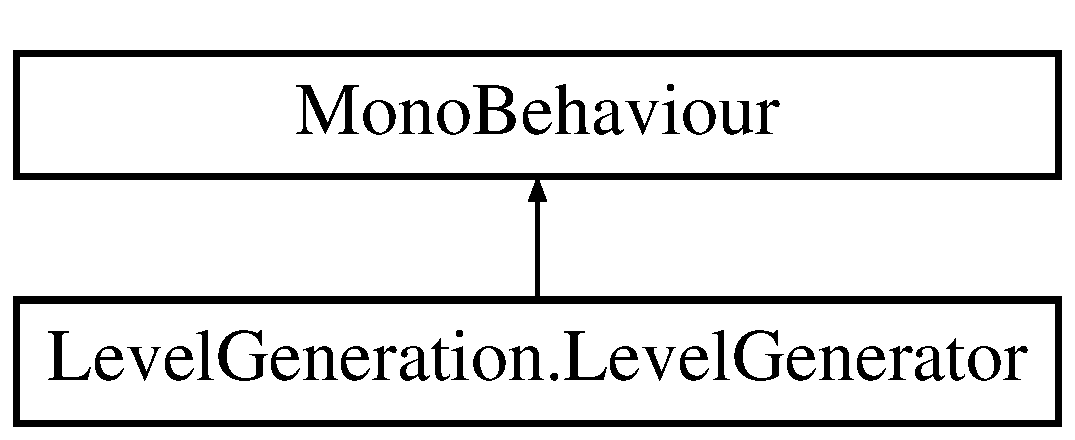
\includegraphics[height=2.000000cm]{class_level_generation_1_1_level_generator}
\end{center}
\end{figure}


\subsection{Detailed Description}
Level generator class that manages the generation process 



Definition at line 10 of file Level\+Generator.\+cs.



The documentation for this class was generated from the following file\+:\begin{DoxyCompactItemize}
\item 
C\+:/\+Users/louca/\+Documents/\+M\+A\+Dissertation/\+M\+A\+Dissertation/\+M\+A\+Dissertation/\+Assets/\+Classes/\+Level Generator/Level\+Generator.\+cs\end{DoxyCompactItemize}

\hypertarget{class_main_menu}{}\section{Main\+Menu Class Reference}
\label{class_main_menu}\index{Main\+Menu@{Main\+Menu}}


A class that controls the main menu  


Inheritance diagram for Main\+Menu\+:\begin{figure}[H]
\begin{center}
\leavevmode
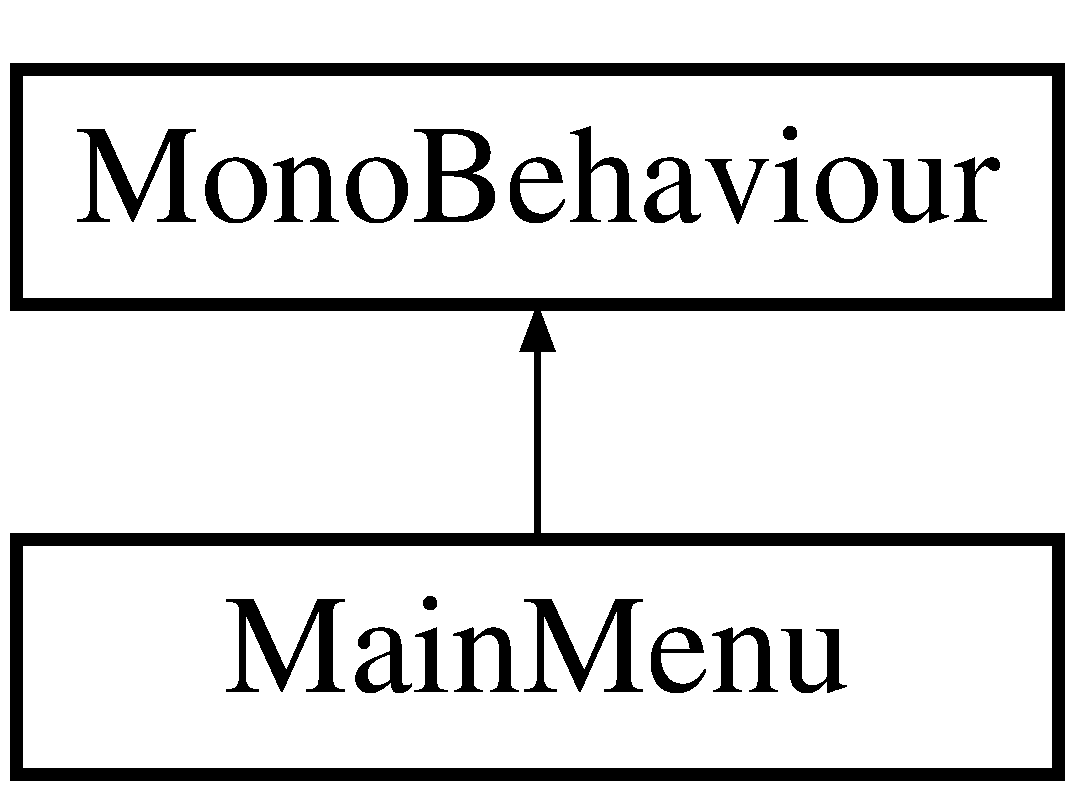
\includegraphics[height=2.000000cm]{class_main_menu}
\end{center}
\end{figure}
\subsection*{Public Member Functions}
\begin{DoxyCompactItemize}
\item 
void \mbox{\hyperlink{class_main_menu_a5e5cf3c9a40d8c3af4a7afb06a4a3f89}{Load\+Game}} ()
\begin{DoxyCompactList}\small\item\em Load the game \end{DoxyCompactList}\item 
void \mbox{\hyperlink{class_main_menu_aeeb49c53aadae1b1608c7d24ea60fca3}{Load\+About}} ()
\begin{DoxyCompactList}\small\item\em Load the about page \end{DoxyCompactList}\item 
void \mbox{\hyperlink{class_main_menu_a2a6f329d1d69aa2ccd1703b061c4d51e}{Exit}} ()
\begin{DoxyCompactList}\small\item\em Exit the game \end{DoxyCompactList}\item 
void \mbox{\hyperlink{class_main_menu_a718238ca30f3203c53cd391a0881e543}{Load\+Questionnaire}} ()
\begin{DoxyCompactList}\small\item\em Load the questionnaire \end{DoxyCompactList}\end{DoxyCompactItemize}


\subsection{Detailed Description}
A class that controls the main menu 



Definition at line 8 of file Main\+Menu.\+cs.



\subsection{Member Function Documentation}
\mbox{\Hypertarget{class_main_menu_a2a6f329d1d69aa2ccd1703b061c4d51e}\label{class_main_menu_a2a6f329d1d69aa2ccd1703b061c4d51e}} 
\index{Main\+Menu@{Main\+Menu}!Exit@{Exit}}
\index{Exit@{Exit}!Main\+Menu@{Main\+Menu}}
\subsubsection{\texorpdfstring{Exit()}{Exit()}}
{\footnotesize\ttfamily void Main\+Menu.\+Exit (\begin{DoxyParamCaption}{ }\end{DoxyParamCaption})}



Exit the game 



Definition at line 39 of file Main\+Menu.\+cs.

\mbox{\Hypertarget{class_main_menu_aeeb49c53aadae1b1608c7d24ea60fca3}\label{class_main_menu_aeeb49c53aadae1b1608c7d24ea60fca3}} 
\index{Main\+Menu@{Main\+Menu}!Load\+About@{Load\+About}}
\index{Load\+About@{Load\+About}!Main\+Menu@{Main\+Menu}}
\subsubsection{\texorpdfstring{Load\+About()}{LoadAbout()}}
{\footnotesize\ttfamily void Main\+Menu.\+Load\+About (\begin{DoxyParamCaption}{ }\end{DoxyParamCaption})}



Load the about page 



Definition at line 31 of file Main\+Menu.\+cs.

\mbox{\Hypertarget{class_main_menu_a5e5cf3c9a40d8c3af4a7afb06a4a3f89}\label{class_main_menu_a5e5cf3c9a40d8c3af4a7afb06a4a3f89}} 
\index{Main\+Menu@{Main\+Menu}!Load\+Game@{Load\+Game}}
\index{Load\+Game@{Load\+Game}!Main\+Menu@{Main\+Menu}}
\subsubsection{\texorpdfstring{Load\+Game()}{LoadGame()}}
{\footnotesize\ttfamily void Main\+Menu.\+Load\+Game (\begin{DoxyParamCaption}{ }\end{DoxyParamCaption})}



Load the game 



Definition at line 23 of file Main\+Menu.\+cs.

\mbox{\Hypertarget{class_main_menu_a718238ca30f3203c53cd391a0881e543}\label{class_main_menu_a718238ca30f3203c53cd391a0881e543}} 
\index{Main\+Menu@{Main\+Menu}!Load\+Questionnaire@{Load\+Questionnaire}}
\index{Load\+Questionnaire@{Load\+Questionnaire}!Main\+Menu@{Main\+Menu}}
\subsubsection{\texorpdfstring{Load\+Questionnaire()}{LoadQuestionnaire()}}
{\footnotesize\ttfamily void Main\+Menu.\+Load\+Questionnaire (\begin{DoxyParamCaption}{ }\end{DoxyParamCaption})}



Load the questionnaire 



Definition at line 47 of file Main\+Menu.\+cs.



The documentation for this class was generated from the following file\+:\begin{DoxyCompactItemize}
\item 
C\+:/\+Users/louca/\+Documents/\+M\+A\+Dissertation/\+M\+A\+Dissertation/\+M\+A\+Dissertation/\+Assets/\+Classes/\+Scene Specific/Main\+Menu.\+cs\end{DoxyCompactItemize}

\hypertarget{class_one_way_platform}{}\section{One\+Way\+Platform Class Reference}
\label{class_one_way_platform}\index{One\+Way\+Platform@{One\+Way\+Platform}}


One way platform class that can be used to switch the platforms collider on and off  


Inheritance diagram for One\+Way\+Platform\+:\begin{figure}[H]
\begin{center}
\leavevmode
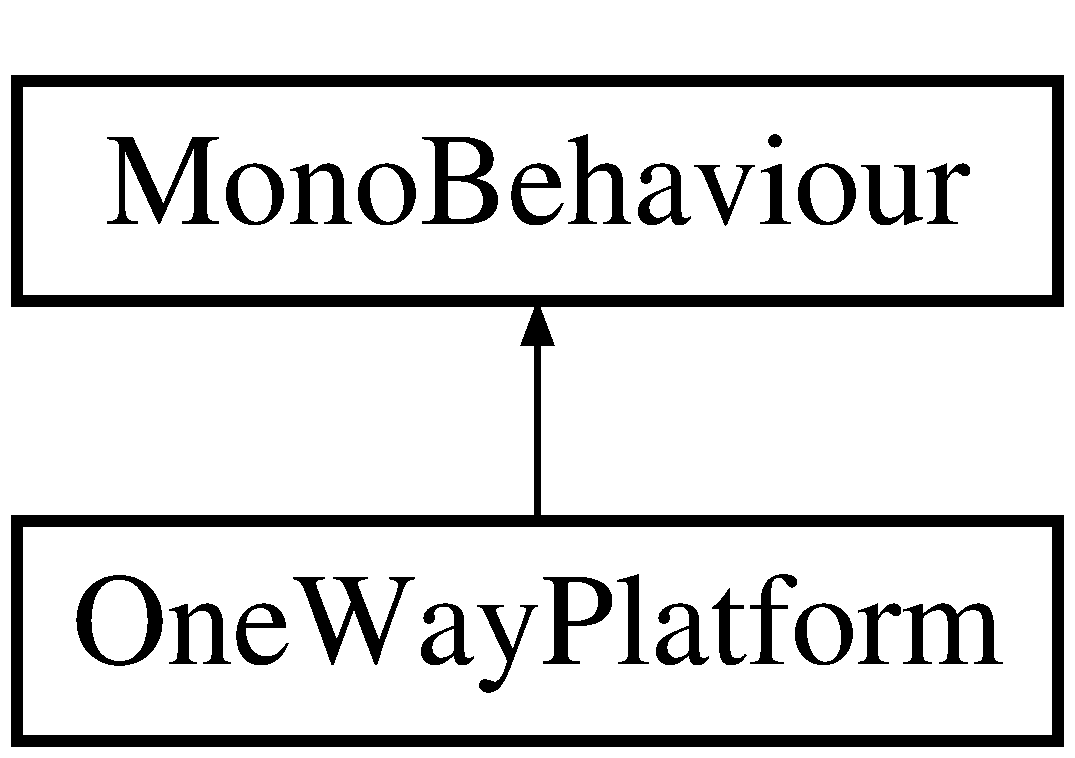
\includegraphics[height=2.000000cm]{class_one_way_platform}
\end{center}
\end{figure}
\subsection*{Public Member Functions}
\begin{DoxyCompactItemize}
\item 
void \mbox{\hyperlink{class_one_way_platform_a10b0da79a1b619409a8186f9766bb810}{Enable\+Solid\+Collider}} ()
\begin{DoxyCompactList}\small\item\em Enable the solid collider \end{DoxyCompactList}\item 
void \mbox{\hyperlink{class_one_way_platform_a1b8029968caa73f149a312d1113d1176}{Disable\+Solid\+Collider}} ()
\begin{DoxyCompactList}\small\item\em Disable the solid collider \end{DoxyCompactList}\item 
I\+Enumerator \mbox{\hyperlink{class_one_way_platform_aa1651ae509037fd1bb7e0bf567f36c60}{Enable\+After}} ()
\begin{DoxyCompactList}\small\item\em Enable the solid collider after X seconds \end{DoxyCompactList}\end{DoxyCompactItemize}


\subsection{Detailed Description}
One way platform class that can be used to switch the platforms collider on and off 



Definition at line 9 of file One\+Way\+Platform.\+cs.



\subsection{Member Function Documentation}
\mbox{\Hypertarget{class_one_way_platform_a1b8029968caa73f149a312d1113d1176}\label{class_one_way_platform_a1b8029968caa73f149a312d1113d1176}} 
\index{One\+Way\+Platform@{One\+Way\+Platform}!Disable\+Solid\+Collider@{Disable\+Solid\+Collider}}
\index{Disable\+Solid\+Collider@{Disable\+Solid\+Collider}!One\+Way\+Platform@{One\+Way\+Platform}}
\subsubsection{\texorpdfstring{Disable\+Solid\+Collider()}{DisableSolidCollider()}}
{\footnotesize\ttfamily void One\+Way\+Platform.\+Disable\+Solid\+Collider (\begin{DoxyParamCaption}{ }\end{DoxyParamCaption})}



Disable the solid collider 



Definition at line 26 of file One\+Way\+Platform.\+cs.

\mbox{\Hypertarget{class_one_way_platform_aa1651ae509037fd1bb7e0bf567f36c60}\label{class_one_way_platform_aa1651ae509037fd1bb7e0bf567f36c60}} 
\index{One\+Way\+Platform@{One\+Way\+Platform}!Enable\+After@{Enable\+After}}
\index{Enable\+After@{Enable\+After}!One\+Way\+Platform@{One\+Way\+Platform}}
\subsubsection{\texorpdfstring{Enable\+After()}{EnableAfter()}}
{\footnotesize\ttfamily I\+Enumerator One\+Way\+Platform.\+Enable\+After (\begin{DoxyParamCaption}{ }\end{DoxyParamCaption})}



Enable the solid collider after X seconds 

\begin{DoxyReturn}{Returns}
Wait For Seconds
\end{DoxyReturn}


Definition at line 35 of file One\+Way\+Platform.\+cs.

\mbox{\Hypertarget{class_one_way_platform_a10b0da79a1b619409a8186f9766bb810}\label{class_one_way_platform_a10b0da79a1b619409a8186f9766bb810}} 
\index{One\+Way\+Platform@{One\+Way\+Platform}!Enable\+Solid\+Collider@{Enable\+Solid\+Collider}}
\index{Enable\+Solid\+Collider@{Enable\+Solid\+Collider}!One\+Way\+Platform@{One\+Way\+Platform}}
\subsubsection{\texorpdfstring{Enable\+Solid\+Collider()}{EnableSolidCollider()}}
{\footnotesize\ttfamily void One\+Way\+Platform.\+Enable\+Solid\+Collider (\begin{DoxyParamCaption}{ }\end{DoxyParamCaption})}



Enable the solid collider 



Definition at line 18 of file One\+Way\+Platform.\+cs.



The documentation for this class was generated from the following file\+:\begin{DoxyCompactItemize}
\item 
C\+:/\+Users/louca/\+Documents/\+M\+A\+Dissertation/\+M\+A\+Dissertation/\+M\+A\+Dissertation/\+Assets/\+Classes/\+Gameplay/One\+Way\+Platform.\+cs\end{DoxyCompactItemize}

\hypertarget{struct_overall_player_data}{}\section{Overall\+Player\+Data Struct Reference}
\label{struct_overall_player_data}\index{Overall\+Player\+Data@{Overall\+Player\+Data}}


Struct to hold all of the play through stats  


\subsection*{Public Attributes}
\begin{DoxyCompactItemize}
\item 
\mbox{\Hypertarget{struct_overall_player_data_a1fd70c56847da7c64bdae2e5b4320467}\label{struct_overall_player_data_a1fd70c56847da7c64bdae2e5b4320467}} 
List$<$ int $>$ {\bfseries m\+\_\+deaths}
\item 
\mbox{\Hypertarget{struct_overall_player_data_aef07934a01be560544a9c373cebe184f}\label{struct_overall_player_data_aef07934a01be560544a9c373cebe184f}} 
List$<$ int $>$ {\bfseries m\+\_\+scores}
\item 
\mbox{\Hypertarget{struct_overall_player_data_a0f890bd5b749843068400cbb8b65cd15}\label{struct_overall_player_data_a0f890bd5b749843068400cbb8b65cd15}} 
List$<$ float $>$ {\bfseries m\+\_\+times}
\end{DoxyCompactItemize}


\subsection{Detailed Description}
Struct to hold all of the play through stats 



Definition at line 782 of file Data\+Tracker.\+cs.



The documentation for this struct was generated from the following file\+:\begin{DoxyCompactItemize}
\item 
C\+:/\+Users/louca/\+Documents/\+M\+A\+Dissertation/\+M\+A\+Dissertation/\+M\+A\+Dissertation/\+Assets/\+Classes/\+Database/Data\+Tracker.\+cs\end{DoxyCompactItemize}

\hypertarget{class_pathing_object}{}\section{Pathing\+Object Class Reference}
\label{class_pathing_object}\index{Pathing\+Object@{Pathing\+Object}}


An object that paths through set points  


Inheritance diagram for Pathing\+Object\+:\begin{figure}[H]
\begin{center}
\leavevmode
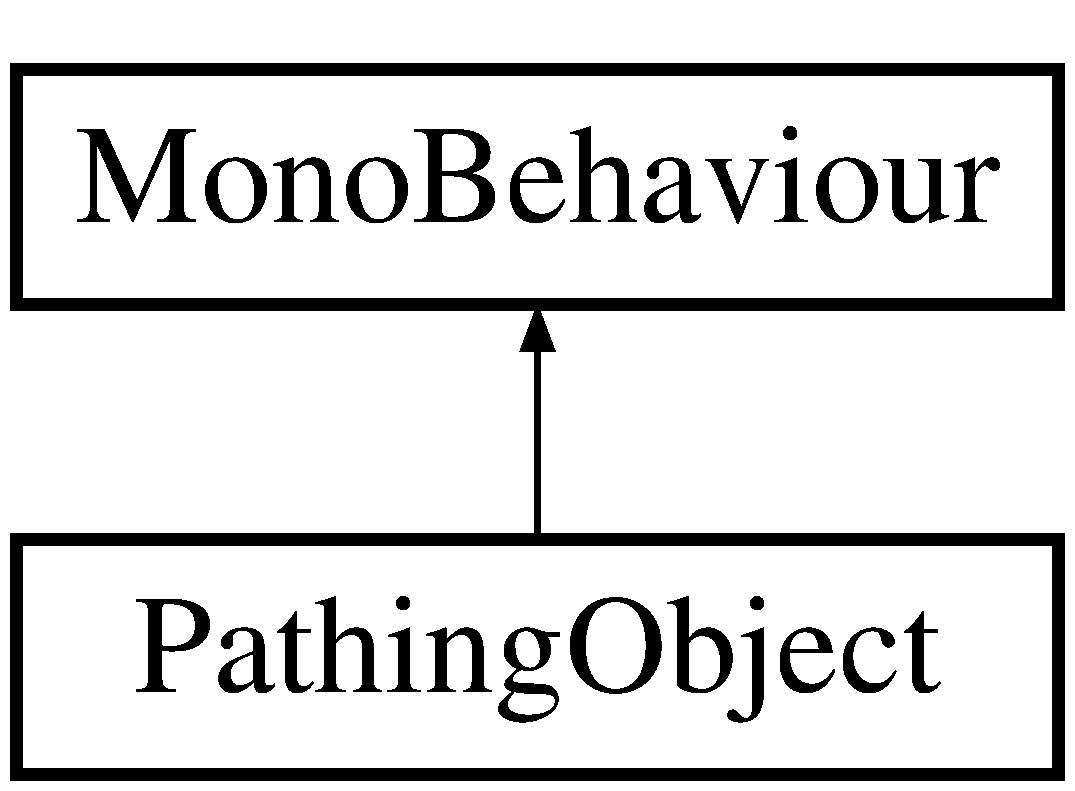
\includegraphics[height=2.000000cm]{class_pathing_object}
\end{center}
\end{figure}


\subsection{Detailed Description}
An object that paths through set points 



Definition at line 8 of file Pathing\+Object.\+cs.



The documentation for this class was generated from the following file\+:\begin{DoxyCompactItemize}
\item 
C\+:/\+Users/louca/\+Documents/\+M\+A\+Dissertation/\+M\+A\+Dissertation/\+M\+A\+Dissertation/\+Assets/\+Classes/\+Gameplay/Pathing\+Object.\+cs\end{DoxyCompactItemize}

\hypertarget{class_player}{}\section{Player Class Reference}
\label{class_player}\index{Player@{Player}}


Human controlled player class  


Inheritance diagram for Player\+:\begin{figure}[H]
\begin{center}
\leavevmode
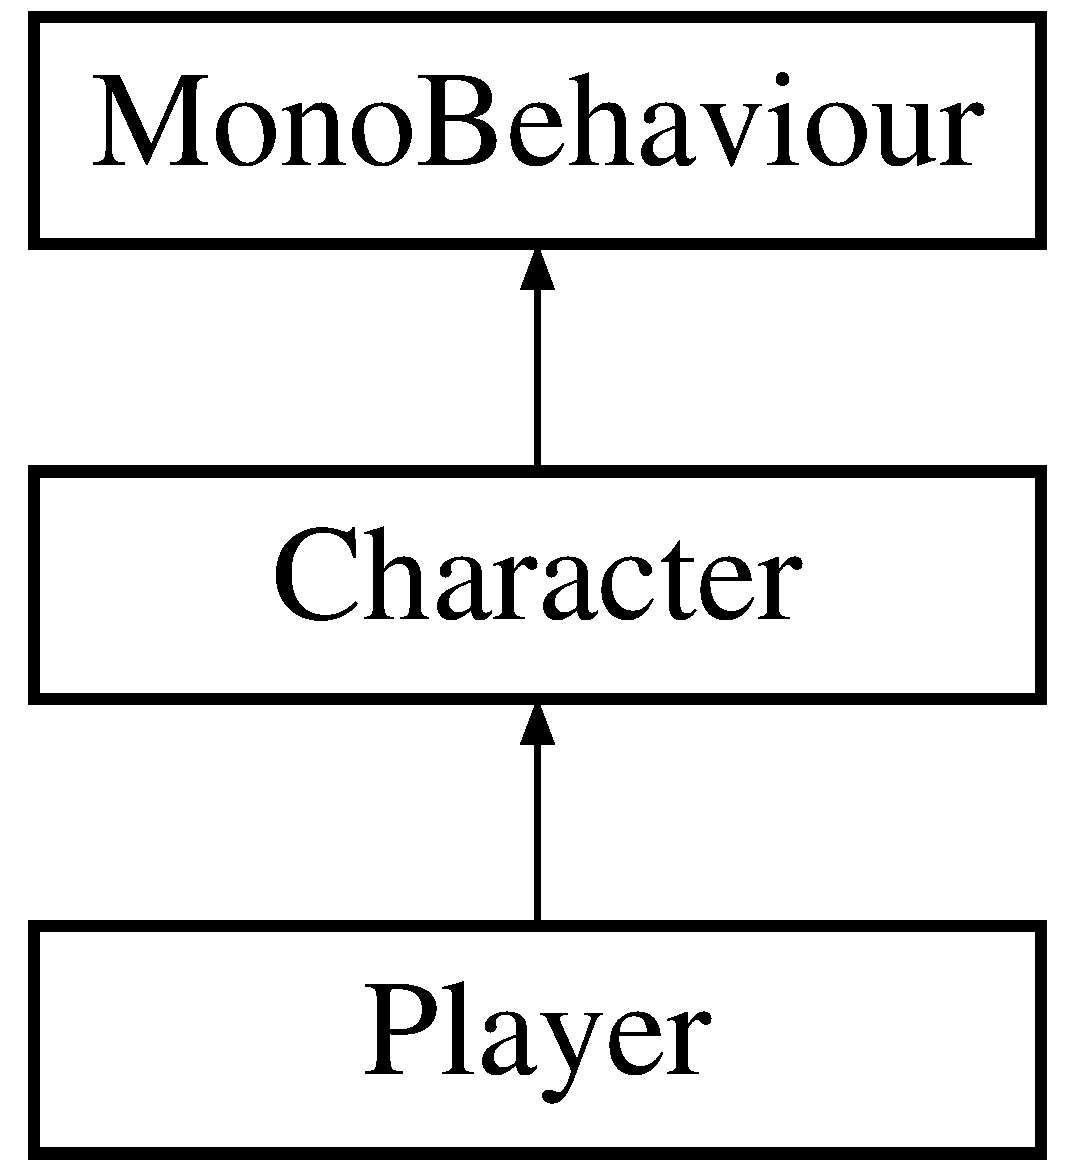
\includegraphics[height=3.000000cm]{class_player}
\end{center}
\end{figure}
\subsection*{Public Member Functions}
\begin{DoxyCompactItemize}
\item 
void \mbox{\hyperlink{class_player_ae4848921e3458e9d0a2cde5acb63e165}{Set\+Camera\+Movement}} (\mbox{\hyperlink{class_camera_movement}{Camera\+Movement}} \+\_\+camera\+Movement)
\begin{DoxyCompactList}\small\item\em Set the camera movement reference \end{DoxyCompactList}\item 
void \mbox{\hyperlink{class_player_a89c5345d4267bf7902531407fe50c61e}{Reset\+Player}} ()
\begin{DoxyCompactList}\small\item\em Reset the player \end{DoxyCompactList}\item 
void \mbox{\hyperlink{class_player_a8e3a84181da3b91573fb395fb8821a90}{Freeze}} ()
\begin{DoxyCompactList}\small\item\em Freeze the player \end{DoxyCompactList}\item 
void \mbox{\hyperlink{class_player_a7a222872698adba22fbd3c90302cc8ca}{Un\+Freeze}} ()
\begin{DoxyCompactList}\small\item\em Unfreeze the player \end{DoxyCompactList}\item 
void \mbox{\hyperlink{class_player_a24f8aeed0a7bb4dc8d2dcceea07dcaf7}{Set\+Current\+Room}} (\mbox{\hyperlink{class_level_generation_1_1_room}{Room}} \+\_\+new\+Room)
\begin{DoxyCompactList}\small\item\em Set the current room the player is in \end{DoxyCompactList}\item 
void \mbox{\hyperlink{class_player_a425c47ab72a45262765b2d60b6636911}{Set\+Spawn}} (Vector3 \+\_\+position)
\begin{DoxyCompactList}\small\item\em Set the spawn position \end{DoxyCompactList}\item 
\mbox{\hyperlink{class_level_generation_1_1_room}{Room}} \mbox{\hyperlink{class_player_ac4bbf69d383242cbf6807fdd28ee0f0d}{Get\+Current\+Room}} ()
\begin{DoxyCompactList}\small\item\em Get the current room the player is in \end{DoxyCompactList}\end{DoxyCompactItemize}
\subsection*{Protected Member Functions}
\begin{DoxyCompactItemize}
\item 
override void \mbox{\hyperlink{class_player_a21d9f4bbd86a4a1aaa8844917270aefb}{Awake}} ()
\begin{DoxyCompactList}\small\item\em Handle Set Up \end{DoxyCompactList}\item 
override void \mbox{\hyperlink{class_player_abccf91b671f93492dfdb704ddf894ae3}{Update}} ()
\begin{DoxyCompactList}\small\item\em Handle Input \end{DoxyCompactList}\item 
override void \mbox{\hyperlink{class_player_a9f719f4557355ff498cc7ff6d3723a84}{Fixed\+Update}} ()
\begin{DoxyCompactList}\small\item\em Handle physics \end{DoxyCompactList}\end{DoxyCompactItemize}
\subsection*{Additional Inherited Members}


\subsection{Detailed Description}
Human controlled player class 



Definition at line 10 of file Player.\+cs.



\subsection{Member Function Documentation}
\mbox{\Hypertarget{class_player_a21d9f4bbd86a4a1aaa8844917270aefb}\label{class_player_a21d9f4bbd86a4a1aaa8844917270aefb}} 
\index{Player@{Player}!Awake@{Awake}}
\index{Awake@{Awake}!Player@{Player}}
\subsubsection{\texorpdfstring{Awake()}{Awake()}}
{\footnotesize\ttfamily override void Player.\+Awake (\begin{DoxyParamCaption}{ }\end{DoxyParamCaption})\hspace{0.3cm}{\ttfamily [protected]}, {\ttfamily [virtual]}}



Handle Set Up 



Reimplemented from \mbox{\hyperlink{class_character_a7cca5d1f141f2f46a1d087fd3e28a953}{Character}}.



Definition at line 79 of file Player.\+cs.

\mbox{\Hypertarget{class_player_a9f719f4557355ff498cc7ff6d3723a84}\label{class_player_a9f719f4557355ff498cc7ff6d3723a84}} 
\index{Player@{Player}!Fixed\+Update@{Fixed\+Update}}
\index{Fixed\+Update@{Fixed\+Update}!Player@{Player}}
\subsubsection{\texorpdfstring{Fixed\+Update()}{FixedUpdate()}}
{\footnotesize\ttfamily override void Player.\+Fixed\+Update (\begin{DoxyParamCaption}{ }\end{DoxyParamCaption})\hspace{0.3cm}{\ttfamily [protected]}, {\ttfamily [virtual]}}



Handle physics 



Reimplemented from \mbox{\hyperlink{class_character_ad90105ab5e234884e5bca7ce5bd2c50e}{Character}}.



Definition at line 248 of file Player.\+cs.

\mbox{\Hypertarget{class_player_a8e3a84181da3b91573fb395fb8821a90}\label{class_player_a8e3a84181da3b91573fb395fb8821a90}} 
\index{Player@{Player}!Freeze@{Freeze}}
\index{Freeze@{Freeze}!Player@{Player}}
\subsubsection{\texorpdfstring{Freeze()}{Freeze()}}
{\footnotesize\ttfamily void Player.\+Freeze (\begin{DoxyParamCaption}{ }\end{DoxyParamCaption})}



Freeze the player 



Definition at line 404 of file Player.\+cs.

\mbox{\Hypertarget{class_player_ac4bbf69d383242cbf6807fdd28ee0f0d}\label{class_player_ac4bbf69d383242cbf6807fdd28ee0f0d}} 
\index{Player@{Player}!Get\+Current\+Room@{Get\+Current\+Room}}
\index{Get\+Current\+Room@{Get\+Current\+Room}!Player@{Player}}
\subsubsection{\texorpdfstring{Get\+Current\+Room()}{GetCurrentRoom()}}
{\footnotesize\ttfamily \mbox{\hyperlink{class_level_generation_1_1_room}{Room}} Player.\+Get\+Current\+Room (\begin{DoxyParamCaption}{ }\end{DoxyParamCaption})}



Get the current room the player is in 

\begin{DoxyReturn}{Returns}
The current room the player is in
\end{DoxyReturn}


Definition at line 451 of file Player.\+cs.

\mbox{\Hypertarget{class_player_a89c5345d4267bf7902531407fe50c61e}\label{class_player_a89c5345d4267bf7902531407fe50c61e}} 
\index{Player@{Player}!Reset\+Player@{Reset\+Player}}
\index{Reset\+Player@{Reset\+Player}!Player@{Player}}
\subsubsection{\texorpdfstring{Reset\+Player()}{ResetPlayer()}}
{\footnotesize\ttfamily void Player.\+Reset\+Player (\begin{DoxyParamCaption}{ }\end{DoxyParamCaption})}



Reset the player 



Definition at line 387 of file Player.\+cs.

\mbox{\Hypertarget{class_player_ae4848921e3458e9d0a2cde5acb63e165}\label{class_player_ae4848921e3458e9d0a2cde5acb63e165}} 
\index{Player@{Player}!Set\+Camera\+Movement@{Set\+Camera\+Movement}}
\index{Set\+Camera\+Movement@{Set\+Camera\+Movement}!Player@{Player}}
\subsubsection{\texorpdfstring{Set\+Camera\+Movement()}{SetCameraMovement()}}
{\footnotesize\ttfamily void Player.\+Set\+Camera\+Movement (\begin{DoxyParamCaption}\item[{\mbox{\hyperlink{class_camera_movement}{Camera\+Movement}}}]{\+\_\+camera\+Movement }\end{DoxyParamCaption})}



Set the camera movement reference 


\begin{DoxyParams}{Parameters}
{\em \+\_\+camera\+Movement} & Camera movement reference\\
\hline
\end{DoxyParams}


Definition at line 101 of file Player.\+cs.

\mbox{\Hypertarget{class_player_a24f8aeed0a7bb4dc8d2dcceea07dcaf7}\label{class_player_a24f8aeed0a7bb4dc8d2dcceea07dcaf7}} 
\index{Player@{Player}!Set\+Current\+Room@{Set\+Current\+Room}}
\index{Set\+Current\+Room@{Set\+Current\+Room}!Player@{Player}}
\subsubsection{\texorpdfstring{Set\+Current\+Room()}{SetCurrentRoom()}}
{\footnotesize\ttfamily void Player.\+Set\+Current\+Room (\begin{DoxyParamCaption}\item[{\mbox{\hyperlink{class_level_generation_1_1_room}{Room}}}]{\+\_\+new\+Room }\end{DoxyParamCaption})}



Set the current room the player is in 


\begin{DoxyParams}{Parameters}
{\em \+\_\+new\+Room} & New current room\\
\hline
\end{DoxyParams}


Definition at line 433 of file Player.\+cs.

\mbox{\Hypertarget{class_player_a425c47ab72a45262765b2d60b6636911}\label{class_player_a425c47ab72a45262765b2d60b6636911}} 
\index{Player@{Player}!Set\+Spawn@{Set\+Spawn}}
\index{Set\+Spawn@{Set\+Spawn}!Player@{Player}}
\subsubsection{\texorpdfstring{Set\+Spawn()}{SetSpawn()}}
{\footnotesize\ttfamily void Player.\+Set\+Spawn (\begin{DoxyParamCaption}\item[{Vector3}]{\+\_\+position }\end{DoxyParamCaption})}



Set the spawn position 


\begin{DoxyParams}{Parameters}
{\em \+\_\+position} & Spawn positon\\
\hline
\end{DoxyParams}


Definition at line 442 of file Player.\+cs.

\mbox{\Hypertarget{class_player_a7a222872698adba22fbd3c90302cc8ca}\label{class_player_a7a222872698adba22fbd3c90302cc8ca}} 
\index{Player@{Player}!Un\+Freeze@{Un\+Freeze}}
\index{Un\+Freeze@{Un\+Freeze}!Player@{Player}}
\subsubsection{\texorpdfstring{Un\+Freeze()}{UnFreeze()}}
{\footnotesize\ttfamily void Player.\+Un\+Freeze (\begin{DoxyParamCaption}{ }\end{DoxyParamCaption})}



Unfreeze the player 



Definition at line 420 of file Player.\+cs.

\mbox{\Hypertarget{class_player_abccf91b671f93492dfdb704ddf894ae3}\label{class_player_abccf91b671f93492dfdb704ddf894ae3}} 
\index{Player@{Player}!Update@{Update}}
\index{Update@{Update}!Player@{Player}}
\subsubsection{\texorpdfstring{Update()}{Update()}}
{\footnotesize\ttfamily override void Player.\+Update (\begin{DoxyParamCaption}{ }\end{DoxyParamCaption})\hspace{0.3cm}{\ttfamily [protected]}, {\ttfamily [virtual]}}



Handle Input 



Reimplemented from \mbox{\hyperlink{class_character}{Character}}.



Definition at line 110 of file Player.\+cs.



The documentation for this class was generated from the following file\+:\begin{DoxyCompactItemize}
\item 
C\+:/\+Users/louca/\+Documents/\+M\+A\+Dissertation/\+M\+A\+Dissertation/\+M\+A\+Dissertation/\+Assets/\+Classes/\+Gameplay/Player.\+cs\end{DoxyCompactItemize}

\hypertarget{struct_player_data}{}\section{Player\+Data Struct Reference}
\label{struct_player_data}\index{Player\+Data@{Player\+Data}}


Struct to hold all of the tracked player data  


\subsection*{Public Attributes}
\begin{DoxyCompactItemize}
\item 
\mbox{\Hypertarget{struct_player_data_a9278645d46293fc45a6c3ec8f9ea3212}\label{struct_player_data_a9278645d46293fc45a6c3ec8f9ea3212}} 
int {\bfseries m\+\_\+current\+Player\+Lives}
\item 
\mbox{\Hypertarget{struct_player_data_aaed7defb7fa33e61a7da04468844232a}\label{struct_player_data_aaed7defb7fa33e61a7da04468844232a}} 
int {\bfseries m\+\_\+current\+Player\+Deaths}
\item 
\mbox{\Hypertarget{struct_player_data_a61b5b35e90b935fa7a6f7280a6c53d8a}\label{struct_player_data_a61b5b35e90b935fa7a6f7280a6c53d8a}} 
float {\bfseries m\+\_\+time\+Taken\+To\+Complete\+Level}
\item 
\mbox{\Hypertarget{struct_player_data_a3b341a1ef8cb96c2570dbf08bb6bed4c}\label{struct_player_data_a3b341a1ef8cb96c2570dbf08bb6bed4c}} 
int {\bfseries m\+\_\+enemies\+Killed}
\item 
\mbox{\Hypertarget{struct_player_data_a95b6e06eada9fc4900b00d35bef4b91c}\label{struct_player_data_a95b6e06eada9fc4900b00d35bef4b91c}} 
int {\bfseries m\+\_\+score}
\item 
\mbox{\Hypertarget{struct_player_data_a9f54dd68b8dc3c4d6f64e99e21b5ae9d}\label{struct_player_data_a9f54dd68b8dc3c4d6f64e99e21b5ae9d}} 
List$<$ \mbox{\hyperlink{struct_simple_room_data}{Simple\+Room\+Data}} $>$ {\bfseries m\+\_\+death\+Room\+Data}
\end{DoxyCompactItemize}


\subsection{Detailed Description}
Struct to hold all of the tracked player data 



Definition at line 711 of file Data\+Tracker.\+cs.



The documentation for this struct was generated from the following file\+:\begin{DoxyCompactItemize}
\item 
C\+:/\+Users/louca/\+Documents/\+M\+A\+Dissertation/\+M\+A\+Dissertation/\+M\+A\+Dissertation/\+Assets/\+Classes/\+Database/Data\+Tracker.\+cs\end{DoxyCompactItemize}

\hypertarget{class_playthrough_data}{}\section{Playthrough\+Data Class Reference}
\label{class_playthrough_data}\index{Playthrough\+Data@{Playthrough\+Data}}


Struct to hold all of the playthrough data  


\subsection*{Public Attributes}
\begin{DoxyCompactItemize}
\item 
\mbox{\Hypertarget{class_playthrough_data_a32c9d72f156f0a9d3a66d05d65f25b21}\label{class_playthrough_data_a32c9d72f156f0a9d3a66d05d65f25b21}} 
int {\bfseries m\+\_\+id}
\item 
\mbox{\Hypertarget{class_playthrough_data_ab4aa6fa0bf0be59b6ee6ef5096fdb1af}\label{class_playthrough_data_ab4aa6fa0bf0be59b6ee6ef5096fdb1af}} 
List$<$ \mbox{\hyperlink{class_level_data}{Level\+Data}} $>$ {\bfseries m\+\_\+level\+Data}
\item 
\mbox{\Hypertarget{class_playthrough_data_afc0d6416b3a39980a610195c9bf26009}\label{class_playthrough_data_afc0d6416b3a39980a610195c9bf26009}} 
int {\bfseries m\+\_\+level\+Id}
\end{DoxyCompactItemize}


\subsection{Detailed Description}
Struct to hold all of the playthrough data 



Definition at line 760 of file Data\+Tracker.\+cs.



The documentation for this class was generated from the following file\+:\begin{DoxyCompactItemize}
\item 
C\+:/\+Users/louca/\+Documents/\+M\+A\+Dissertation/\+M\+A\+Dissertation/\+M\+A\+Dissertation/\+Assets/\+Classes/\+Database/Data\+Tracker.\+cs\end{DoxyCompactItemize}

\hypertarget{class_level_generation_1_1_room}{}\section{Level\+Generation.\+Room Class Reference}
\label{class_level_generation_1_1_room}\index{Level\+Generation.\+Room@{Level\+Generation.\+Room}}


\mbox{\hyperlink{class_level_generation_1_1_room}{Room}} class that controls customisation and linking between other rooms  


Inheritance diagram for Level\+Generation.\+Room\+:\begin{figure}[H]
\begin{center}
\leavevmode
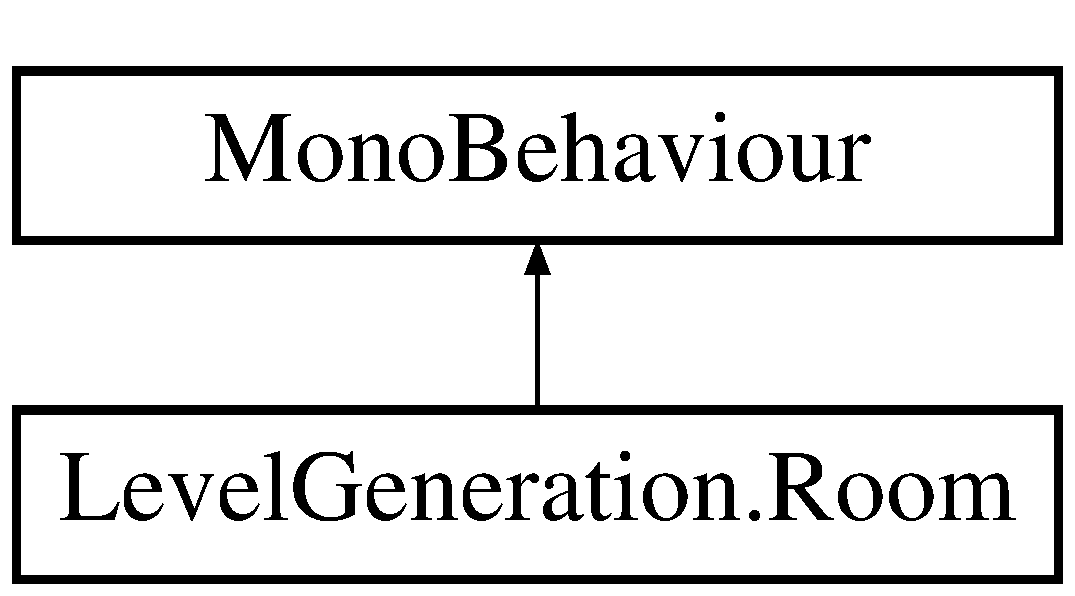
\includegraphics[height=2.000000cm]{class_level_generation_1_1_room}
\end{center}
\end{figure}
\subsection*{Public Member Functions}
\begin{DoxyCompactItemize}
\item 
void \mbox{\hyperlink{class_level_generation_1_1_room_ac54baebea1ec085f79843e5c42a66467}{Init}} (\mbox{\hyperlink{namespace_level_generation_a206451e0c8bfced86ae4b9348cd3718f}{Room\+Type}} \+\_\+type, Vector2\+Int \+\_\+position)
\begin{DoxyCompactList}\small\item\em Initialise the room with room type and grid position \end{DoxyCompactList}\item 
void \mbox{\hyperlink{class_level_generation_1_1_room_ac4d1b1b285ac602653b1810eb09492fd}{Set\+Room\+Type}} (\mbox{\hyperlink{namespace_level_generation_a206451e0c8bfced86ae4b9348cd3718f}{Room\+Type}} \+\_\+type)
\begin{DoxyCompactList}\small\item\em Set the room type \end{DoxyCompactList}\item 
void \mbox{\hyperlink{class_level_generation_1_1_room_ae07be6a48b5fa0b1eff3b2ed08be2206}{Set\+Connection\+Type}} (\mbox{\hyperlink{namespace_level_generation_ac48934e101078b19dce3479d82f689e0}{Connection\+Type}} \+\_\+type)
\begin{DoxyCompactList}\small\item\em Set the connection type \end{DoxyCompactList}\item 
\mbox{\hyperlink{namespace_level_generation_a206451e0c8bfced86ae4b9348cd3718f}{Room\+Type}} \mbox{\hyperlink{class_level_generation_1_1_room_aff17f63f58338e84997627bcaed08afc}{Get\+Room\+Type}} ()
\begin{DoxyCompactList}\small\item\em Get the room type \end{DoxyCompactList}\item 
Vector2\+Int \mbox{\hyperlink{class_level_generation_1_1_room_abfd82aaf18d4332f843635b9790af3d7}{Get\+Position}} ()
\begin{DoxyCompactList}\small\item\em Get the room position \end{DoxyCompactList}\item 
void \mbox{\hyperlink{class_level_generation_1_1_room_ae6cd86347ce784fab849c28cf4a70be9}{Link\+Rooms}} (string \+\_\+connection, \mbox{\hyperlink{class_level_generation_1_1_room}{Room}} \+\_\+connected\+Room)
\begin{DoxyCompactList}\small\item\em Link the two rooms together \end{DoxyCompactList}\item 
void \mbox{\hyperlink{class_level_generation_1_1_room_adfc209b5289f68c3c105e1590a4dd652}{Attempt\+Spawn\+Collectable}} (ref int \+\_\+current\+Count, int \+\_\+collectable\+Count\+Max)
\begin{DoxyCompactList}\small\item\em Attempt to spawn a collectable in the room \end{DoxyCompactList}\item 
void \mbox{\hyperlink{class_level_generation_1_1_room_ae87c91e9280cfb6043c6d3bfe720d1ef}{Enable\+End\+Zone}} ()
\begin{DoxyCompactList}\small\item\em Enable the end zone game object \end{DoxyCompactList}\item 
Transform \mbox{\hyperlink{class_level_generation_1_1_room_a3c9be1844b28b37af37ab01e199361d0}{Get\+Spawn\+Position}} ()
\begin{DoxyCompactList}\small\item\em Get the player spawn position \end{DoxyCompactList}\end{DoxyCompactItemize}


\subsection{Detailed Description}
\mbox{\hyperlink{class_level_generation_1_1_room}{Room}} class that controls customisation and linking between other rooms 



Definition at line 10 of file Room.\+cs.



\subsection{Member Function Documentation}
\mbox{\Hypertarget{class_level_generation_1_1_room_adfc209b5289f68c3c105e1590a4dd652}\label{class_level_generation_1_1_room_adfc209b5289f68c3c105e1590a4dd652}} 
\index{Level\+Generation\+::\+Room@{Level\+Generation\+::\+Room}!Attempt\+Spawn\+Collectable@{Attempt\+Spawn\+Collectable}}
\index{Attempt\+Spawn\+Collectable@{Attempt\+Spawn\+Collectable}!Level\+Generation\+::\+Room@{Level\+Generation\+::\+Room}}
\subsubsection{\texorpdfstring{Attempt\+Spawn\+Collectable()}{AttemptSpawnCollectable()}}
{\footnotesize\ttfamily void Level\+Generation.\+Room.\+Attempt\+Spawn\+Collectable (\begin{DoxyParamCaption}\item[{ref int}]{\+\_\+current\+Count,  }\item[{int}]{\+\_\+collectable\+Count\+Max }\end{DoxyParamCaption})}



Attempt to spawn a collectable in the room 


\begin{DoxyParams}{Parameters}
{\em \+\_\+current\+Count} & Current collectable count\\
\hline
{\em \+\_\+collectable\+Count\+Max} & Max amount of collectables that can spawn\\
\hline
\end{DoxyParams}


Definition at line 286 of file Room.\+cs.

\mbox{\Hypertarget{class_level_generation_1_1_room_ae87c91e9280cfb6043c6d3bfe720d1ef}\label{class_level_generation_1_1_room_ae87c91e9280cfb6043c6d3bfe720d1ef}} 
\index{Level\+Generation\+::\+Room@{Level\+Generation\+::\+Room}!Enable\+End\+Zone@{Enable\+End\+Zone}}
\index{Enable\+End\+Zone@{Enable\+End\+Zone}!Level\+Generation\+::\+Room@{Level\+Generation\+::\+Room}}
\subsubsection{\texorpdfstring{Enable\+End\+Zone()}{EnableEndZone()}}
{\footnotesize\ttfamily void Level\+Generation.\+Room.\+Enable\+End\+Zone (\begin{DoxyParamCaption}{ }\end{DoxyParamCaption})}



Enable the end zone game object 



Definition at line 313 of file Room.\+cs.

\mbox{\Hypertarget{class_level_generation_1_1_room_abfd82aaf18d4332f843635b9790af3d7}\label{class_level_generation_1_1_room_abfd82aaf18d4332f843635b9790af3d7}} 
\index{Level\+Generation\+::\+Room@{Level\+Generation\+::\+Room}!Get\+Position@{Get\+Position}}
\index{Get\+Position@{Get\+Position}!Level\+Generation\+::\+Room@{Level\+Generation\+::\+Room}}
\subsubsection{\texorpdfstring{Get\+Position()}{GetPosition()}}
{\footnotesize\ttfamily Vector2\+Int Level\+Generation.\+Room.\+Get\+Position (\begin{DoxyParamCaption}{ }\end{DoxyParamCaption})}



Get the room position 

\begin{DoxyReturn}{Returns}
\mbox{\hyperlink{class_level_generation_1_1_room}{Room}} position
\end{DoxyReturn}


Definition at line 240 of file Room.\+cs.

\mbox{\Hypertarget{class_level_generation_1_1_room_aff17f63f58338e84997627bcaed08afc}\label{class_level_generation_1_1_room_aff17f63f58338e84997627bcaed08afc}} 
\index{Level\+Generation\+::\+Room@{Level\+Generation\+::\+Room}!Get\+Room\+Type@{Get\+Room\+Type}}
\index{Get\+Room\+Type@{Get\+Room\+Type}!Level\+Generation\+::\+Room@{Level\+Generation\+::\+Room}}
\subsubsection{\texorpdfstring{Get\+Room\+Type()}{GetRoomType()}}
{\footnotesize\ttfamily \mbox{\hyperlink{namespace_level_generation_a206451e0c8bfced86ae4b9348cd3718f}{Room\+Type}} Level\+Generation.\+Room.\+Get\+Room\+Type (\begin{DoxyParamCaption}{ }\end{DoxyParamCaption})}



Get the room type 

\begin{DoxyReturn}{Returns}
\mbox{\hyperlink{class_level_generation_1_1_room}{Room}} type
\end{DoxyReturn}


Definition at line 231 of file Room.\+cs.

\mbox{\Hypertarget{class_level_generation_1_1_room_a3c9be1844b28b37af37ab01e199361d0}\label{class_level_generation_1_1_room_a3c9be1844b28b37af37ab01e199361d0}} 
\index{Level\+Generation\+::\+Room@{Level\+Generation\+::\+Room}!Get\+Spawn\+Position@{Get\+Spawn\+Position}}
\index{Get\+Spawn\+Position@{Get\+Spawn\+Position}!Level\+Generation\+::\+Room@{Level\+Generation\+::\+Room}}
\subsubsection{\texorpdfstring{Get\+Spawn\+Position()}{GetSpawnPosition()}}
{\footnotesize\ttfamily Transform Level\+Generation.\+Room.\+Get\+Spawn\+Position (\begin{DoxyParamCaption}{ }\end{DoxyParamCaption})}



Get the player spawn position 

\begin{DoxyReturn}{Returns}
\mbox{\hyperlink{class_player}{Player}} spawn position
\end{DoxyReturn}


Definition at line 322 of file Room.\+cs.

\mbox{\Hypertarget{class_level_generation_1_1_room_ac54baebea1ec085f79843e5c42a66467}\label{class_level_generation_1_1_room_ac54baebea1ec085f79843e5c42a66467}} 
\index{Level\+Generation\+::\+Room@{Level\+Generation\+::\+Room}!Init@{Init}}
\index{Init@{Init}!Level\+Generation\+::\+Room@{Level\+Generation\+::\+Room}}
\subsubsection{\texorpdfstring{Init()}{Init()}}
{\footnotesize\ttfamily void Level\+Generation.\+Room.\+Init (\begin{DoxyParamCaption}\item[{\mbox{\hyperlink{namespace_level_generation_a206451e0c8bfced86ae4b9348cd3718f}{Room\+Type}}}]{\+\_\+type,  }\item[{Vector2\+Int}]{\+\_\+position }\end{DoxyParamCaption})}



Initialise the room with room type and grid position 


\begin{DoxyParams}{Parameters}
{\em \+\_\+type} & \\
\hline
{\em \+\_\+position} & \\
\hline
\end{DoxyParams}


Definition at line 92 of file Room.\+cs.

\mbox{\Hypertarget{class_level_generation_1_1_room_ae6cd86347ce784fab849c28cf4a70be9}\label{class_level_generation_1_1_room_ae6cd86347ce784fab849c28cf4a70be9}} 
\index{Level\+Generation\+::\+Room@{Level\+Generation\+::\+Room}!Link\+Rooms@{Link\+Rooms}}
\index{Link\+Rooms@{Link\+Rooms}!Level\+Generation\+::\+Room@{Level\+Generation\+::\+Room}}
\subsubsection{\texorpdfstring{Link\+Rooms()}{LinkRooms()}}
{\footnotesize\ttfamily void Level\+Generation.\+Room.\+Link\+Rooms (\begin{DoxyParamCaption}\item[{string}]{\+\_\+connection,  }\item[{\mbox{\hyperlink{class_level_generation_1_1_room}{Room}}}]{\+\_\+connected\+Room }\end{DoxyParamCaption})}



Link the two rooms together 


\begin{DoxyParams}{Parameters}
{\em \+\_\+connection} & Connection string\\
\hline
{\em \+\_\+connected\+Room} & Connected \mbox{\hyperlink{class_level_generation_1_1_room}{Room}}\\
\hline
\end{DoxyParams}


Definition at line 250 of file Room.\+cs.

\mbox{\Hypertarget{class_level_generation_1_1_room_ae07be6a48b5fa0b1eff3b2ed08be2206}\label{class_level_generation_1_1_room_ae07be6a48b5fa0b1eff3b2ed08be2206}} 
\index{Level\+Generation\+::\+Room@{Level\+Generation\+::\+Room}!Set\+Connection\+Type@{Set\+Connection\+Type}}
\index{Set\+Connection\+Type@{Set\+Connection\+Type}!Level\+Generation\+::\+Room@{Level\+Generation\+::\+Room}}
\subsubsection{\texorpdfstring{Set\+Connection\+Type()}{SetConnectionType()}}
{\footnotesize\ttfamily void Level\+Generation.\+Room.\+Set\+Connection\+Type (\begin{DoxyParamCaption}\item[{\mbox{\hyperlink{namespace_level_generation_ac48934e101078b19dce3479d82f689e0}{Connection\+Type}}}]{\+\_\+type }\end{DoxyParamCaption})}



Set the connection type 


\begin{DoxyParams}{Parameters}
{\em \+\_\+type} & \\
\hline
\end{DoxyParams}


Definition at line 166 of file Room.\+cs.

\mbox{\Hypertarget{class_level_generation_1_1_room_ac4d1b1b285ac602653b1810eb09492fd}\label{class_level_generation_1_1_room_ac4d1b1b285ac602653b1810eb09492fd}} 
\index{Level\+Generation\+::\+Room@{Level\+Generation\+::\+Room}!Set\+Room\+Type@{Set\+Room\+Type}}
\index{Set\+Room\+Type@{Set\+Room\+Type}!Level\+Generation\+::\+Room@{Level\+Generation\+::\+Room}}
\subsubsection{\texorpdfstring{Set\+Room\+Type()}{SetRoomType()}}
{\footnotesize\ttfamily void Level\+Generation.\+Room.\+Set\+Room\+Type (\begin{DoxyParamCaption}\item[{\mbox{\hyperlink{namespace_level_generation_a206451e0c8bfced86ae4b9348cd3718f}{Room\+Type}}}]{\+\_\+type }\end{DoxyParamCaption})}



Set the room type 


\begin{DoxyParams}{Parameters}
{\em \+\_\+type} & \\
\hline
\end{DoxyParams}


Definition at line 128 of file Room.\+cs.



The documentation for this class was generated from the following file\+:\begin{DoxyCompactItemize}
\item 
C\+:/\+Users/louca/\+Documents/\+M\+A\+Dissertation/\+M\+A\+Dissertation/\+M\+A\+Dissertation/\+Assets/\+Classes/\+Gameplay/Room.\+cs\end{DoxyCompactItemize}

\hypertarget{class_room_exit}{}\section{Room\+Exit Class Reference}
\label{class_room_exit}\index{Room\+Exit@{Room\+Exit}}


Used to help transition from room to room  


Inheritance diagram for Room\+Exit\+:\begin{figure}[H]
\begin{center}
\leavevmode
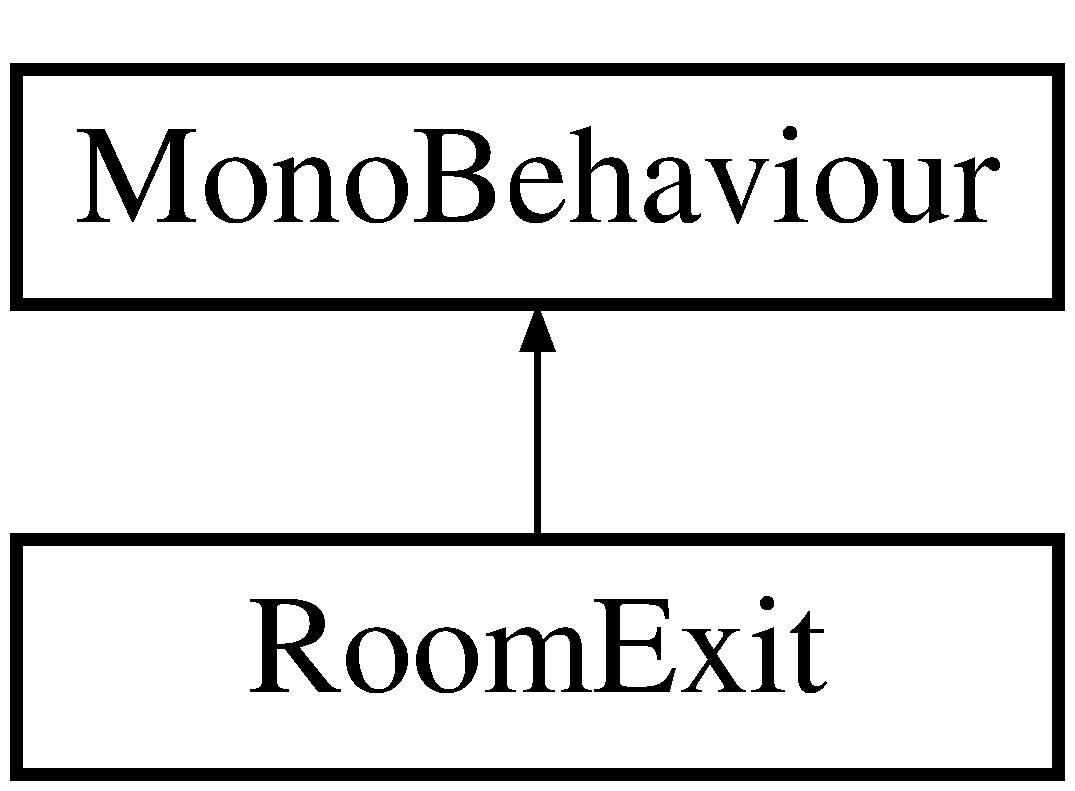
\includegraphics[height=2.000000cm]{class_room_exit}
\end{center}
\end{figure}
\subsection*{Public Member Functions}
\begin{DoxyCompactItemize}
\item 
void \mbox{\hyperlink{class_room_exit_adfc62765726e94628e9f04191d940a04}{Set\+Connected\+Room}} (\mbox{\hyperlink{class_level_generation_1_1_room}{Room}} \+\_\+room)
\begin{DoxyCompactList}\small\item\em Set the connected room \end{DoxyCompactList}\item 
\mbox{\hyperlink{class_level_generation_1_1_room}{Room}} \mbox{\hyperlink{class_room_exit_a43eb9678e9d5a584e124d88d7da03d52}{Get\+Room}} ()
\begin{DoxyCompactList}\small\item\em Access the connected room \end{DoxyCompactList}\end{DoxyCompactItemize}


\subsection{Detailed Description}
Used to help transition from room to room 



Definition at line 9 of file Room\+Exit.\+cs.



\subsection{Member Function Documentation}
\mbox{\Hypertarget{class_room_exit_a43eb9678e9d5a584e124d88d7da03d52}\label{class_room_exit_a43eb9678e9d5a584e124d88d7da03d52}} 
\index{Room\+Exit@{Room\+Exit}!Get\+Room@{Get\+Room}}
\index{Get\+Room@{Get\+Room}!Room\+Exit@{Room\+Exit}}
\subsubsection{\texorpdfstring{Get\+Room()}{GetRoom()}}
{\footnotesize\ttfamily \mbox{\hyperlink{class_level_generation_1_1_room}{Room}} Room\+Exit.\+Get\+Room (\begin{DoxyParamCaption}{ }\end{DoxyParamCaption})}



Access the connected room 

\begin{DoxyReturn}{Returns}

\end{DoxyReturn}


Definition at line 28 of file Room\+Exit.\+cs.

\mbox{\Hypertarget{class_room_exit_adfc62765726e94628e9f04191d940a04}\label{class_room_exit_adfc62765726e94628e9f04191d940a04}} 
\index{Room\+Exit@{Room\+Exit}!Set\+Connected\+Room@{Set\+Connected\+Room}}
\index{Set\+Connected\+Room@{Set\+Connected\+Room}!Room\+Exit@{Room\+Exit}}
\subsubsection{\texorpdfstring{Set\+Connected\+Room()}{SetConnectedRoom()}}
{\footnotesize\ttfamily void Room\+Exit.\+Set\+Connected\+Room (\begin{DoxyParamCaption}\item[{\mbox{\hyperlink{class_level_generation_1_1_room}{Room}}}]{\+\_\+room }\end{DoxyParamCaption})}



Set the connected room 


\begin{DoxyParams}{Parameters}
{\em \+\_\+room} & \\
\hline
\end{DoxyParams}


Definition at line 19 of file Room\+Exit.\+cs.



The documentation for this class was generated from the following file\+:\begin{DoxyCompactItemize}
\item 
C\+:/\+Users/louca/\+Documents/\+M\+A\+Dissertation/\+M\+A\+Dissertation/\+M\+A\+Dissertation/\+Assets/\+Classes/\+Gameplay/Room\+Exit.\+cs\end{DoxyCompactItemize}

\hypertarget{struct_scene_data}{}\section{Scene\+Data Struct Reference}
\label{struct_scene_data}\index{Scene\+Data@{Scene\+Data}}


Struct that stores various scene data values  


\subsection*{Public Attributes}
\begin{DoxyCompactItemize}
\item 
\mbox{\Hypertarget{struct_scene_data_a21525ac0e4967dd28c90f423bdf8082f}\label{struct_scene_data_a21525ac0e4967dd28c90f423bdf8082f}} 
string {\bfseries m\+\_\+scene\+Name}
\item 
\mbox{\Hypertarget{struct_scene_data_a090335ef7fb48d46b1fec4a37b2f112d}\label{struct_scene_data_a090335ef7fb48d46b1fec4a37b2f112d}} 
int {\bfseries m\+\_\+scene\+Index}
\item 
\mbox{\Hypertarget{struct_scene_data_a06a2ef794bb7dccc71f5748983685969}\label{struct_scene_data_a06a2ef794bb7dccc71f5748983685969}} 
bool {\bfseries m\+\_\+load\+A\+Sync}
\end{DoxyCompactItemize}


\subsection{Detailed Description}
Struct that stores various scene data values 



Definition at line 57 of file Main\+Menu.\+cs.



The documentation for this struct was generated from the following file\+:\begin{DoxyCompactItemize}
\item 
C\+:/\+Users/louca/\+Documents/\+M\+A\+Dissertation/\+M\+A\+Dissertation/\+M\+A\+Dissertation/\+Assets/\+Classes/\+Scene Specific/Main\+Menu.\+cs\end{DoxyCompactItemize}

\hypertarget{class_scene_loader}{}\section{Scene\+Loader Class Reference}
\label{class_scene_loader}\index{Scene\+Loader@{Scene\+Loader}}


Singleton class that can be used to load other scenes  


Inheritance diagram for Scene\+Loader\+:\begin{figure}[H]
\begin{center}
\leavevmode
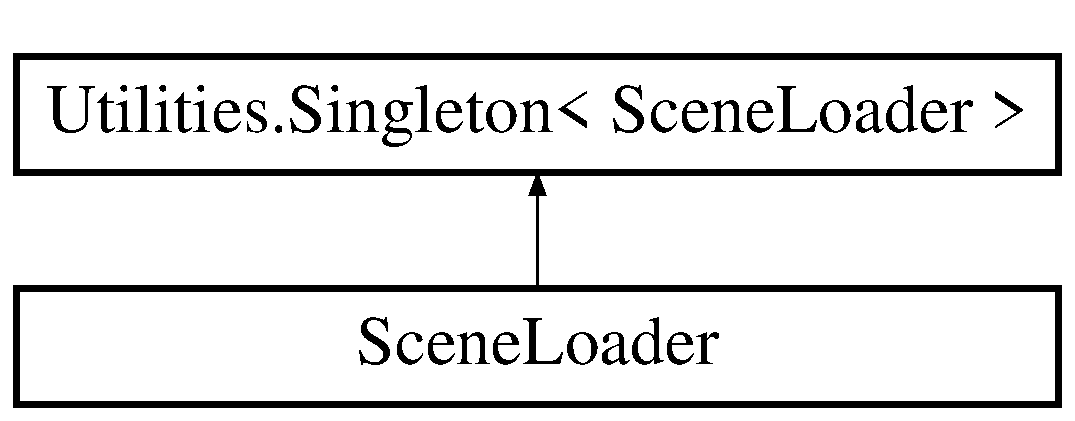
\includegraphics[height=2.000000cm]{class_scene_loader}
\end{center}
\end{figure}
\subsection*{Public Member Functions}
\begin{DoxyCompactItemize}
\item 
void \mbox{\hyperlink{class_scene_loader_a163293de6da9b9a1fd0f0814dec77973}{Load\+Scene}} (string \+\_\+scene\+Name)
\begin{DoxyCompactList}\small\item\em Load a scene \end{DoxyCompactList}\item 
void \mbox{\hyperlink{class_scene_loader_a13020def59e988030b5a019fe31baaa3}{Load\+Scene}} (int \+\_\+scene\+Index)
\begin{DoxyCompactList}\small\item\em Load a scene \end{DoxyCompactList}\item 
void \mbox{\hyperlink{class_scene_loader_ae19ae9a4206c64852c9538d0671dbe96}{Load\+Scene\+A\+Sync}} (string \+\_\+scene\+Name)
\begin{DoxyCompactList}\small\item\em Load a scene using A-\/sync \end{DoxyCompactList}\item 
void \mbox{\hyperlink{class_scene_loader_a13e9697bd4f96b57e215d179b85767f5}{Load\+Scene\+A\+Sync}} (int \+\_\+scene\+Index)
\begin{DoxyCompactList}\small\item\em Load a scene using A-\/sync \end{DoxyCompactList}\item 
void \mbox{\hyperlink{class_scene_loader_a0e53114fa65d1ef71d1c6af0bcb4fde5}{Exit\+Game}} ()
\begin{DoxyCompactList}\small\item\em Exit the game \end{DoxyCompactList}\end{DoxyCompactItemize}
\subsection*{Additional Inherited Members}


\subsection{Detailed Description}
Singleton class that can be used to load other scenes 



Definition at line 10 of file Scene\+Loader.\+cs.



\subsection{Member Function Documentation}
\mbox{\Hypertarget{class_scene_loader_a0e53114fa65d1ef71d1c6af0bcb4fde5}\label{class_scene_loader_a0e53114fa65d1ef71d1c6af0bcb4fde5}} 
\index{Scene\+Loader@{Scene\+Loader}!Exit\+Game@{Exit\+Game}}
\index{Exit\+Game@{Exit\+Game}!Scene\+Loader@{Scene\+Loader}}
\subsubsection{\texorpdfstring{Exit\+Game()}{ExitGame()}}
{\footnotesize\ttfamily void Scene\+Loader.\+Exit\+Game (\begin{DoxyParamCaption}{ }\end{DoxyParamCaption})}



Exit the game 



Definition at line 51 of file Scene\+Loader.\+cs.

\mbox{\Hypertarget{class_scene_loader_a163293de6da9b9a1fd0f0814dec77973}\label{class_scene_loader_a163293de6da9b9a1fd0f0814dec77973}} 
\index{Scene\+Loader@{Scene\+Loader}!Load\+Scene@{Load\+Scene}}
\index{Load\+Scene@{Load\+Scene}!Scene\+Loader@{Scene\+Loader}}
\subsubsection{\texorpdfstring{Load\+Scene()}{LoadScene()}\hspace{0.1cm}{\footnotesize\ttfamily [1/2]}}
{\footnotesize\ttfamily void Scene\+Loader.\+Load\+Scene (\begin{DoxyParamCaption}\item[{string}]{\+\_\+scene\+Name }\end{DoxyParamCaption})}



Load a scene 


\begin{DoxyParams}{Parameters}
{\em \+\_\+scene\+Name} & Scene Name\\
\hline
\end{DoxyParams}


Definition at line 16 of file Scene\+Loader.\+cs.

\mbox{\Hypertarget{class_scene_loader_a13020def59e988030b5a019fe31baaa3}\label{class_scene_loader_a13020def59e988030b5a019fe31baaa3}} 
\index{Scene\+Loader@{Scene\+Loader}!Load\+Scene@{Load\+Scene}}
\index{Load\+Scene@{Load\+Scene}!Scene\+Loader@{Scene\+Loader}}
\subsubsection{\texorpdfstring{Load\+Scene()}{LoadScene()}\hspace{0.1cm}{\footnotesize\ttfamily [2/2]}}
{\footnotesize\ttfamily void Scene\+Loader.\+Load\+Scene (\begin{DoxyParamCaption}\item[{int}]{\+\_\+scene\+Index }\end{DoxyParamCaption})}



Load a scene 


\begin{DoxyParams}{Parameters}
{\em \+\_\+scene\+Index} & Scene Index\\
\hline
\end{DoxyParams}


Definition at line 25 of file Scene\+Loader.\+cs.

\mbox{\Hypertarget{class_scene_loader_ae19ae9a4206c64852c9538d0671dbe96}\label{class_scene_loader_ae19ae9a4206c64852c9538d0671dbe96}} 
\index{Scene\+Loader@{Scene\+Loader}!Load\+Scene\+A\+Sync@{Load\+Scene\+A\+Sync}}
\index{Load\+Scene\+A\+Sync@{Load\+Scene\+A\+Sync}!Scene\+Loader@{Scene\+Loader}}
\subsubsection{\texorpdfstring{Load\+Scene\+A\+Sync()}{LoadSceneASync()}\hspace{0.1cm}{\footnotesize\ttfamily [1/2]}}
{\footnotesize\ttfamily void Scene\+Loader.\+Load\+Scene\+A\+Sync (\begin{DoxyParamCaption}\item[{string}]{\+\_\+scene\+Name }\end{DoxyParamCaption})}



Load a scene using A-\/sync 


\begin{DoxyParams}{Parameters}
{\em \+\_\+scene\+Name} & Scene Name\\
\hline
\end{DoxyParams}


Definition at line 34 of file Scene\+Loader.\+cs.

\mbox{\Hypertarget{class_scene_loader_a13e9697bd4f96b57e215d179b85767f5}\label{class_scene_loader_a13e9697bd4f96b57e215d179b85767f5}} 
\index{Scene\+Loader@{Scene\+Loader}!Load\+Scene\+A\+Sync@{Load\+Scene\+A\+Sync}}
\index{Load\+Scene\+A\+Sync@{Load\+Scene\+A\+Sync}!Scene\+Loader@{Scene\+Loader}}
\subsubsection{\texorpdfstring{Load\+Scene\+A\+Sync()}{LoadSceneASync()}\hspace{0.1cm}{\footnotesize\ttfamily [2/2]}}
{\footnotesize\ttfamily void Scene\+Loader.\+Load\+Scene\+A\+Sync (\begin{DoxyParamCaption}\item[{int}]{\+\_\+scene\+Index }\end{DoxyParamCaption})}



Load a scene using A-\/sync 


\begin{DoxyParams}{Parameters}
{\em \+\_\+scene\+Index} & Scene Index\\
\hline
\end{DoxyParams}


Definition at line 43 of file Scene\+Loader.\+cs.



The documentation for this class was generated from the following file\+:\begin{DoxyCompactItemize}
\item 
C\+:/\+Users/louca/\+Documents/\+M\+A\+Dissertation/\+M\+A\+Dissertation/\+M\+A\+Dissertation/\+Assets/\+Classes/\+Utils/Scene\+Loader.\+cs\end{DoxyCompactItemize}

\hypertarget{class_screenshot}{}\section{Screenshot Class Reference}
\label{class_screenshot}\index{Screenshot@{Screenshot}}


A class that allows screenshots to be taken  


Inheritance diagram for Screenshot\+:\begin{figure}[H]
\begin{center}
\leavevmode
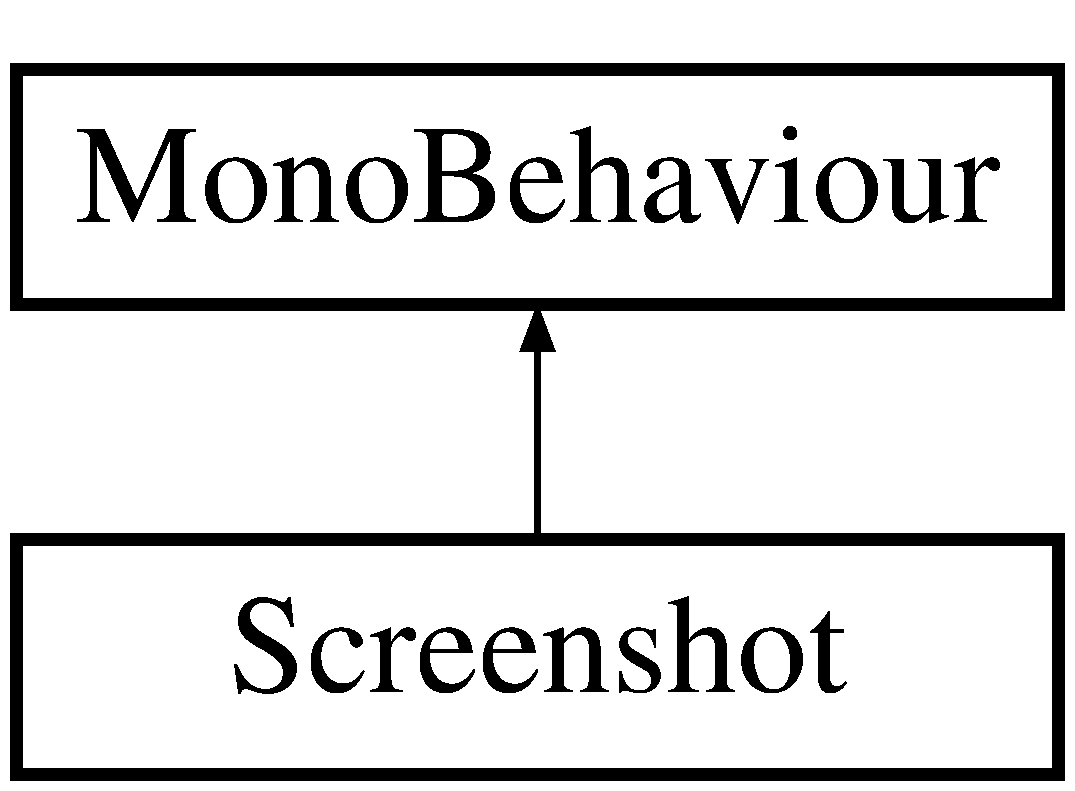
\includegraphics[height=2.000000cm]{class_screenshot}
\end{center}
\end{figure}
\subsection*{Public Attributes}
\begin{DoxyCompactItemize}
\item 
\mbox{\Hypertarget{class_screenshot_a21c1f3172a2ddda552690a011bc94ec8}\label{class_screenshot_a21c1f3172a2ddda552690a011bc94ec8}} 
string {\bfseries m\+\_\+filename}
\item 
\mbox{\Hypertarget{class_screenshot_a9abe9d95f9a5e9a70be2f02ab546fc06}\label{class_screenshot_a9abe9d95f9a5e9a70be2f02ab546fc06}} 
int {\bfseries m\+\_\+super\+Size} = 1
\item 
\mbox{\Hypertarget{class_screenshot_a3c00ae9816a0b25218639edbe5a2c9df}\label{class_screenshot_a3c00ae9816a0b25218639edbe5a2c9df}} 
Key\+Code {\bfseries m\+\_\+screenshot\+Key}
\end{DoxyCompactItemize}


\subsection{Detailed Description}
A class that allows screenshots to be taken 



Definition at line 8 of file Screenshot.\+cs.



The documentation for this class was generated from the following file\+:\begin{DoxyCompactItemize}
\item 
C\+:/\+Users/louca/\+Documents/\+M\+A\+Dissertation/\+M\+A\+Dissertation/\+M\+A\+Dissertation/\+Assets/\+Classes/\+Utils/Screenshot.\+cs\end{DoxyCompactItemize}

\hypertarget{struct_simple_room_data}{}\section{Simple\+Room\+Data Struct Reference}
\label{struct_simple_room_data}\index{Simple\+Room\+Data@{Simple\+Room\+Data}}


Struct to hold a simplified version of a rooms data  


\subsection*{Public Attributes}
\begin{DoxyCompactItemize}
\item 
\mbox{\Hypertarget{struct_simple_room_data_ac80e688a9bad8937da529273c913ecff}\label{struct_simple_room_data_ac80e688a9bad8937da529273c913ecff}} 
int {\bfseries m\+\_\+x\+Pos}
\item 
\mbox{\Hypertarget{struct_simple_room_data_a37ba4564682f18286647606797e0956f}\label{struct_simple_room_data_a37ba4564682f18286647606797e0956f}} 
int {\bfseries m\+\_\+y\+Pos}
\item 
\mbox{\Hypertarget{struct_simple_room_data_ac024ae430b6bd0f2e2ffca2fa9fbfb43}\label{struct_simple_room_data_ac024ae430b6bd0f2e2ffca2fa9fbfb43}} 
string {\bfseries m\+\_\+letter\+Representative}
\item 
\mbox{\Hypertarget{struct_simple_room_data_a838ada358f16225cdf39a2cddc753a15}\label{struct_simple_room_data_a838ada358f16225cdf39a2cddc753a15}} 
string {\bfseries m\+\_\+prefab\+Name}
\end{DoxyCompactItemize}


\subsection{Detailed Description}
Struct to hold a simplified version of a rooms data 



Definition at line 737 of file Data\+Tracker.\+cs.



The documentation for this struct was generated from the following file\+:\begin{DoxyCompactItemize}
\item 
C\+:/\+Users/louca/\+Documents/\+M\+A\+Dissertation/\+M\+A\+Dissertation/\+M\+A\+Dissertation/\+Assets/\+Classes/\+Database/Data\+Tracker.\+cs\end{DoxyCompactItemize}

\hypertarget{class_utilities_1_1_singleton}{}\section{Utilities.\+Singleton$<$ T $>$ Class Template Reference}
\label{class_utilities_1_1_singleton}\index{Utilities.\+Singleton$<$ T $>$@{Utilities.\+Singleton$<$ T $>$}}


\mbox{\hyperlink{class_utilities_1_1_singleton}{Singleton}} behaviour class, used for components that should only have one instance.  


Inheritance diagram for Utilities.\+Singleton$<$ T $>$\+:\begin{figure}[H]
\begin{center}
\leavevmode
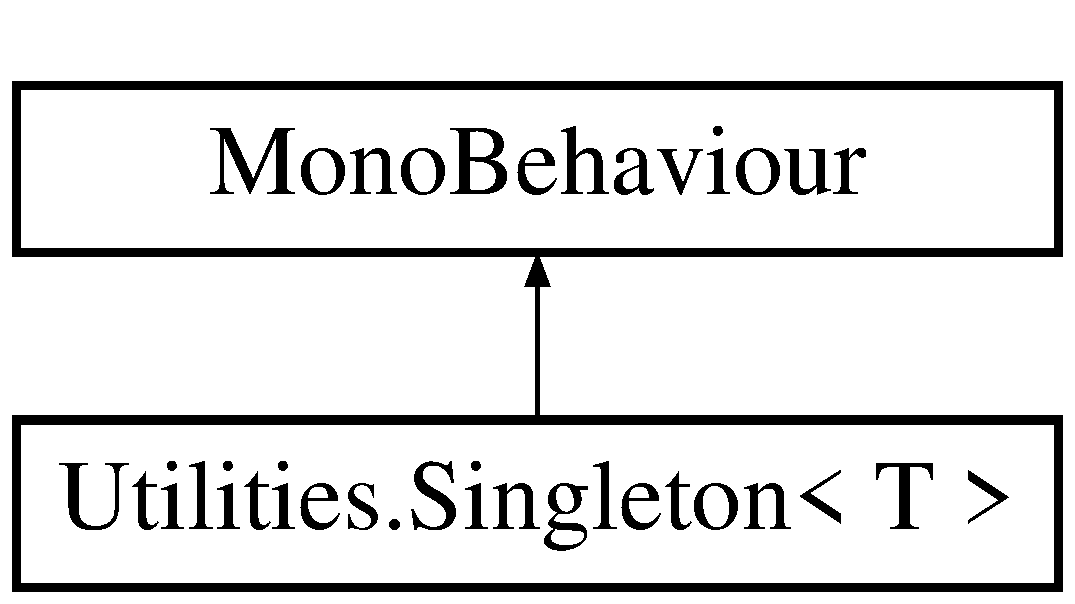
\includegraphics[height=2.000000cm]{class_utilities_1_1_singleton}
\end{center}
\end{figure}
\subsection*{Static Public Member Functions}
\begin{DoxyCompactItemize}
\item 
\mbox{\Hypertarget{class_utilities_1_1_singleton_a123c0df7e7714b113a68d48f1d247a04}\label{class_utilities_1_1_singleton_a123c0df7e7714b113a68d48f1d247a04}} 
static void {\bfseries Assert\+Is\+Initialized} ()
\end{DoxyCompactItemize}
\subsection*{Protected Member Functions}
\begin{DoxyCompactItemize}
\item 
virtual void \mbox{\hyperlink{class_utilities_1_1_singleton_a634b915d7ac492899512de602d59e650}{Awake}} ()
\begin{DoxyCompactList}\small\item\em Base Awake method that sets the \mbox{\hyperlink{class_utilities_1_1_singleton}{Singleton}}\textquotesingle{}s unique instance. Called by Unity when initializing a Mono\+Behaviour. Scripts that extend \mbox{\hyperlink{class_utilities_1_1_singleton}{Singleton}} should be sure to call base.\+Awake() to ensure the static Instance reference is properly created. \end{DoxyCompactList}\item 
virtual void \mbox{\hyperlink{class_utilities_1_1_singleton_a2f20e07021a39a041e87e1a4906c77cb}{On\+Destroy}} ()
\begin{DoxyCompactList}\small\item\em Base On\+Destroy method that destroys the \mbox{\hyperlink{class_utilities_1_1_singleton}{Singleton}}\textquotesingle{}s unique instance. Called by Unity when destroying a Mono\+Behaviour. Scripts that extend \mbox{\hyperlink{class_utilities_1_1_singleton}{Singleton}} should be sure to call base.\+On\+Destroy() to ensure the underlying static Instance reference is properly cleaned up. \end{DoxyCompactList}\end{DoxyCompactItemize}
\subsection*{Properties}
\begin{DoxyCompactItemize}
\item 
static T \mbox{\hyperlink{class_utilities_1_1_singleton_a7b33f3dfee9e78908ad67a0b80eb3a61}{Instance}}\hspace{0.3cm}{\ttfamily  \mbox{[}get\mbox{]}}
\begin{DoxyCompactList}\small\item\em Returns the \mbox{\hyperlink{class_utilities_1_1_singleton}{Singleton}} instance of the classes type. If no instance is found, then we search for an instance in the scene. If more than one instance is found, we throw an error and no instance is returned. \end{DoxyCompactList}\item 
static bool \mbox{\hyperlink{class_utilities_1_1_singleton_ae3d28b0d6fbd2091235b2b2cd17a4c9a}{Is\+Initialized}}\hspace{0.3cm}{\ttfamily  \mbox{[}get\mbox{]}}
\begin{DoxyCompactList}\small\item\em Returns whether the instance has been initialized or not. \end{DoxyCompactList}\end{DoxyCompactItemize}


\subsection{Detailed Description}
\mbox{\hyperlink{class_utilities_1_1_singleton}{Singleton}} behaviour class, used for components that should only have one instance. 

\mbox{\hyperlink{class_utilities_1_1_singleton}{Singleton}} classes live on through scene transitions and will mark their parent root Game\+Object with Object.\+Dont\+Destroy\+On\+Load


\begin{DoxyTemplParams}{Template Parameters}
{\em T} & The \mbox{\hyperlink{class_utilities_1_1_singleton}{Singleton}} Type\\
\hline
\end{DoxyTemplParams}
\begin{Desc}
\item[Type Constraints]\begin{description}
\item[{\em T} : {\em \mbox{\hyperlink{class_utilities_1_1_singleton}{Singleton}}$<$T$>$}]\end{description}
\end{Desc}


Definition at line 14 of file Singleton.\+cs.



\subsection{Member Function Documentation}
\mbox{\Hypertarget{class_utilities_1_1_singleton_a634b915d7ac492899512de602d59e650}\label{class_utilities_1_1_singleton_a634b915d7ac492899512de602d59e650}} 
\index{Utilities\+::\+Singleton@{Utilities\+::\+Singleton}!Awake@{Awake}}
\index{Awake@{Awake}!Utilities\+::\+Singleton@{Utilities\+::\+Singleton}}
\subsubsection{\texorpdfstring{Awake()}{Awake()}}
{\footnotesize\ttfamily virtual void \mbox{\hyperlink{class_utilities_1_1_singleton}{Utilities.\+Singleton}}$<$ T $>$.Awake (\begin{DoxyParamCaption}{ }\end{DoxyParamCaption})\hspace{0.3cm}{\ttfamily [protected]}, {\ttfamily [virtual]}}



Base Awake method that sets the \mbox{\hyperlink{class_utilities_1_1_singleton}{Singleton}}\textquotesingle{}s unique instance. Called by Unity when initializing a Mono\+Behaviour. Scripts that extend \mbox{\hyperlink{class_utilities_1_1_singleton}{Singleton}} should be sure to call base.\+Awake() to ensure the static Instance reference is properly created. 



Reimplemented in \mbox{\hyperlink{class_data_tracker_a683df3af0a4675dc96498519641f6c53}{Data\+Tracker}}, and \mbox{\hyperlink{class_database_manager_ab6b2a5348b157b217b1ee38a468a3167}{Database\+Manager}}.



Definition at line 73 of file Singleton.\+cs.

\mbox{\Hypertarget{class_utilities_1_1_singleton_a2f20e07021a39a041e87e1a4906c77cb}\label{class_utilities_1_1_singleton_a2f20e07021a39a041e87e1a4906c77cb}} 
\index{Utilities\+::\+Singleton@{Utilities\+::\+Singleton}!On\+Destroy@{On\+Destroy}}
\index{On\+Destroy@{On\+Destroy}!Utilities\+::\+Singleton@{Utilities\+::\+Singleton}}
\subsubsection{\texorpdfstring{On\+Destroy()}{OnDestroy()}}
{\footnotesize\ttfamily virtual void \mbox{\hyperlink{class_utilities_1_1_singleton}{Utilities.\+Singleton}}$<$ T $>$.On\+Destroy (\begin{DoxyParamCaption}{ }\end{DoxyParamCaption})\hspace{0.3cm}{\ttfamily [protected]}, {\ttfamily [virtual]}}



Base On\+Destroy method that destroys the \mbox{\hyperlink{class_utilities_1_1_singleton}{Singleton}}\textquotesingle{}s unique instance. Called by Unity when destroying a Mono\+Behaviour. Scripts that extend \mbox{\hyperlink{class_utilities_1_1_singleton}{Singleton}} should be sure to call base.\+On\+Destroy() to ensure the underlying static Instance reference is properly cleaned up. 



Definition at line 110 of file Singleton.\+cs.



\subsection{Property Documentation}
\mbox{\Hypertarget{class_utilities_1_1_singleton_a7b33f3dfee9e78908ad67a0b80eb3a61}\label{class_utilities_1_1_singleton_a7b33f3dfee9e78908ad67a0b80eb3a61}} 
\index{Utilities\+::\+Singleton@{Utilities\+::\+Singleton}!Instance@{Instance}}
\index{Instance@{Instance}!Utilities\+::\+Singleton@{Utilities\+::\+Singleton}}
\subsubsection{\texorpdfstring{Instance}{Instance}}
{\footnotesize\ttfamily T \mbox{\hyperlink{class_utilities_1_1_singleton}{Utilities.\+Singleton}}$<$ T $>$.Instance\hspace{0.3cm}{\ttfamily [static]}, {\ttfamily [get]}}



Returns the \mbox{\hyperlink{class_utilities_1_1_singleton}{Singleton}} instance of the classes type. If no instance is found, then we search for an instance in the scene. If more than one instance is found, we throw an error and no instance is returned. 



Definition at line 29 of file Singleton.\+cs.

\mbox{\Hypertarget{class_utilities_1_1_singleton_ae3d28b0d6fbd2091235b2b2cd17a4c9a}\label{class_utilities_1_1_singleton_ae3d28b0d6fbd2091235b2b2cd17a4c9a}} 
\index{Utilities\+::\+Singleton@{Utilities\+::\+Singleton}!Is\+Initialized@{Is\+Initialized}}
\index{Is\+Initialized@{Is\+Initialized}!Utilities\+::\+Singleton@{Utilities\+::\+Singleton}}
\subsubsection{\texorpdfstring{Is\+Initialized}{IsInitialized}}
{\footnotesize\ttfamily bool \mbox{\hyperlink{class_utilities_1_1_singleton}{Utilities.\+Singleton}}$<$ T $>$.Is\+Initialized\hspace{0.3cm}{\ttfamily [static]}, {\ttfamily [get]}}



Returns whether the instance has been initialized or not. 



Definition at line 60 of file Singleton.\+cs.



The documentation for this class was generated from the following file\+:\begin{DoxyCompactItemize}
\item 
C\+:/\+Users/louca/\+Documents/\+M\+A\+Dissertation/\+M\+A\+Dissertation/\+M\+A\+Dissertation/\+Assets/\+Classes/\+Utils/Singleton.\+cs\end{DoxyCompactItemize}

\hypertarget{class_level_generation_1_1_template_group}{}\section{Level\+Generation.\+Template\+Group Class Reference}
\label{class_level_generation_1_1_template_group}\index{Level\+Generation.\+Template\+Group@{Level\+Generation.\+Template\+Group}}


A class that stores data related to the groups difficulty  


\subsection*{Public Attributes}
\begin{DoxyCompactItemize}
\item 
\mbox{\Hypertarget{class_level_generation_1_1_template_group_ae5ff3aa455059ea023fe9914b261f464}\label{class_level_generation_1_1_template_group_ae5ff3aa455059ea023fe9914b261f464}} 
string {\bfseries m\+\_\+group\+Name}
\item 
\mbox{\Hypertarget{class_level_generation_1_1_template_group_af8fe8d7ab9c3f9904d5b3a51134a3dc4}\label{class_level_generation_1_1_template_group_af8fe8d7ab9c3f9904d5b3a51134a3dc4}} 
Difficulty {\bfseries m\+\_\+difficulty}
\item 
\mbox{\Hypertarget{class_level_generation_1_1_template_group_a08669e71dc903a1dd580affa2b8fe4f3}\label{class_level_generation_1_1_template_group_a08669e71dc903a1dd580affa2b8fe4f3}} 
Game\+Object \mbox{[}$\,$\mbox{]} {\bfseries m\+\_\+room\+Prefabs}
\item 
\mbox{\Hypertarget{class_level_generation_1_1_template_group_a51b2ad45dad9e7297bd0a5107a31cf8c}\label{class_level_generation_1_1_template_group_a51b2ad45dad9e7297bd0a5107a31cf8c}} 
Vector2\+Int {\bfseries m\+\_\+grid\+Min\+Max}
\item 
\mbox{\Hypertarget{class_level_generation_1_1_template_group_adcfec59890e32f28d0e6850eb4fc4bbf}\label{class_level_generation_1_1_template_group_adcfec59890e32f28d0e6850eb4fc4bbf}} 
int {\bfseries m\+\_\+collectable\+Count}
\item 
\mbox{\Hypertarget{class_level_generation_1_1_template_group_ac9df41e2a7437e8b8890eb077afe61d7}\label{class_level_generation_1_1_template_group_ac9df41e2a7437e8b8890eb077afe61d7}} 
\mbox{\hyperlink{struct_level_generation_1_1_data_averages}{Data\+Averages}} {\bfseries m\+\_\+deaths\+Averages}
\item 
\mbox{\Hypertarget{class_level_generation_1_1_template_group_a20a0ae17362f673fc6e4115eda6ff3d2}\label{class_level_generation_1_1_template_group_a20a0ae17362f673fc6e4115eda6ff3d2}} 
\mbox{\hyperlink{struct_level_generation_1_1_data_averages}{Data\+Averages}} {\bfseries m\+\_\+score\+Averages}
\item 
\mbox{\Hypertarget{class_level_generation_1_1_template_group_aa6aeb32ba96b0de00f326d136b5a9abf}\label{class_level_generation_1_1_template_group_aa6aeb32ba96b0de00f326d136b5a9abf}} 
\mbox{\hyperlink{struct_level_generation_1_1_data_averages}{Data\+Averages}} {\bfseries m\+\_\+time\+Averages}
\end{DoxyCompactItemize}


\subsection{Detailed Description}
A class that stores data related to the groups difficulty 



Definition at line 58 of file Template\+Holder.\+cs.



The documentation for this class was generated from the following file\+:\begin{DoxyCompactItemize}
\item 
C\+:/\+Users/louca/\+Documents/\+M\+A\+Dissertation/\+M\+A\+Dissertation/\+M\+A\+Dissertation/\+Assets/\+Classes/\+Level Generator/Template\+Holder.\+cs\end{DoxyCompactItemize}

\hypertarget{class_level_generation_1_1_template_holder}{}\section{Level\+Generation.\+Template\+Holder Class Reference}
\label{class_level_generation_1_1_template_holder}\index{Level\+Generation.\+Template\+Holder@{Level\+Generation.\+Template\+Holder}}


A scriptable object that holds all of the different difficulty groups data such as the room prefabs, grid sizes and averages  


Inheritance diagram for Level\+Generation.\+Template\+Holder\+:\begin{figure}[H]
\begin{center}
\leavevmode
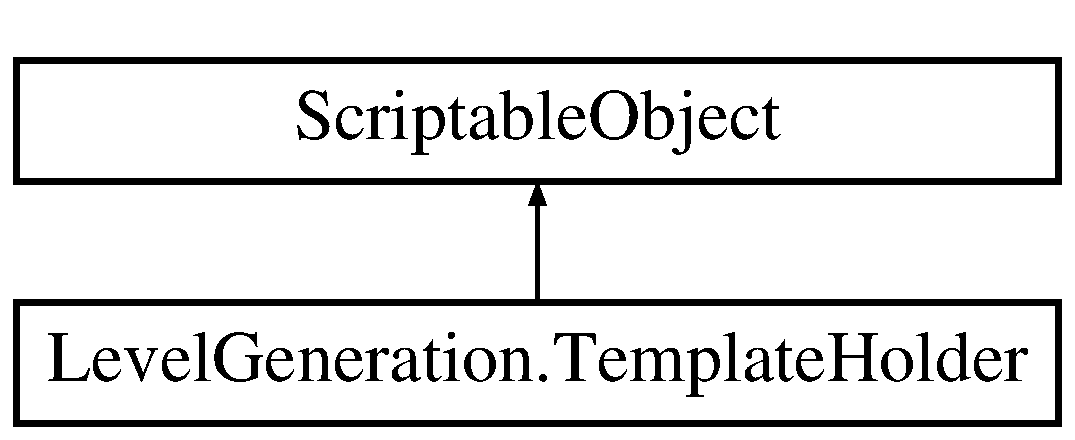
\includegraphics[height=2.000000cm]{class_level_generation_1_1_template_holder}
\end{center}
\end{figure}
\subsection*{Public Member Functions}
\begin{DoxyCompactItemize}
\item 
List$<$ \mbox{\hyperlink{class_level_generation_1_1_template_group}{Template\+Group}} $>$ \mbox{\hyperlink{class_level_generation_1_1_template_holder_a7bf3b585f3b2a6de8b5c0b32f34786ce}{Get\+Template\+Groups}} ()
\begin{DoxyCompactList}\small\item\em Access all of the template groups \end{DoxyCompactList}\item 
\mbox{\hyperlink{class_level_generation_1_1_template_group}{Template\+Group}} \mbox{\hyperlink{class_level_generation_1_1_template_holder_ad2e43ac2d95bff2cc2ac9afdc9cccc8e}{Ge\+Template\+Group}} (Difficulty \+\_\+current\+Difficulty)
\begin{DoxyCompactList}\small\item\em Access a specific template group \end{DoxyCompactList}\end{DoxyCompactItemize}


\subsection{Detailed Description}
A scriptable object that holds all of the different difficulty groups data such as the room prefabs, grid sizes and averages 



Definition at line 12 of file Template\+Holder.\+cs.



\subsection{Member Function Documentation}
\mbox{\Hypertarget{class_level_generation_1_1_template_holder_ad2e43ac2d95bff2cc2ac9afdc9cccc8e}\label{class_level_generation_1_1_template_holder_ad2e43ac2d95bff2cc2ac9afdc9cccc8e}} 
\index{Level\+Generation\+::\+Template\+Holder@{Level\+Generation\+::\+Template\+Holder}!Ge\+Template\+Group@{Ge\+Template\+Group}}
\index{Ge\+Template\+Group@{Ge\+Template\+Group}!Level\+Generation\+::\+Template\+Holder@{Level\+Generation\+::\+Template\+Holder}}
\subsubsection{\texorpdfstring{Ge\+Template\+Group()}{GeTemplateGroup()}}
{\footnotesize\ttfamily \mbox{\hyperlink{class_level_generation_1_1_template_group}{Template\+Group}} Level\+Generation.\+Template\+Holder.\+Ge\+Template\+Group (\begin{DoxyParamCaption}\item[{Difficulty}]{\+\_\+current\+Difficulty }\end{DoxyParamCaption})}



Access a specific template group 


\begin{DoxyParams}{Parameters}
{\em \+\_\+current\+Difficulty} & The current difficulty\\
\hline
\end{DoxyParams}
\begin{DoxyReturn}{Returns}
A specific template group
\end{DoxyReturn}


Definition at line 32 of file Template\+Holder.\+cs.

\mbox{\Hypertarget{class_level_generation_1_1_template_holder_a7bf3b585f3b2a6de8b5c0b32f34786ce}\label{class_level_generation_1_1_template_holder_a7bf3b585f3b2a6de8b5c0b32f34786ce}} 
\index{Level\+Generation\+::\+Template\+Holder@{Level\+Generation\+::\+Template\+Holder}!Get\+Template\+Groups@{Get\+Template\+Groups}}
\index{Get\+Template\+Groups@{Get\+Template\+Groups}!Level\+Generation\+::\+Template\+Holder@{Level\+Generation\+::\+Template\+Holder}}
\subsubsection{\texorpdfstring{Get\+Template\+Groups()}{GetTemplateGroups()}}
{\footnotesize\ttfamily List$<$\mbox{\hyperlink{class_level_generation_1_1_template_group}{Template\+Group}}$>$ Level\+Generation.\+Template\+Holder.\+Get\+Template\+Groups (\begin{DoxyParamCaption}{ }\end{DoxyParamCaption})}



Access all of the template groups 

\begin{DoxyReturn}{Returns}
A list of template groups
\end{DoxyReturn}


Definition at line 22 of file Template\+Holder.\+cs.



The documentation for this class was generated from the following file\+:\begin{DoxyCompactItemize}
\item 
C\+:/\+Users/louca/\+Documents/\+M\+A\+Dissertation/\+M\+A\+Dissertation/\+M\+A\+Dissertation/\+Assets/\+Classes/\+Level Generator/Template\+Holder.\+cs\end{DoxyCompactItemize}

%--- End generated contents ---

% Index
\backmatter
\newpage
\phantomsection
\clearemptydoublepage
\addcontentsline{toc}{chapter}{Index}
\printindex

\end{document}
